\chapter{Euclidian Geometry}
\setcounter{figure}{1}
\setcounter{subfigure}{1}
\section{Geometry Revision}
\setcounter{figure}{1}
\setcounter{subfigure}{1}

Geometry (from the Greek ``geo`` = earth and ``metria`` = measure) arose as the field of knowledge
dealing with spatial relationships. Geometry can be split into Euclidean geometry and analytical geometry. 
Analtyical geometry deals with space and shape in an algebraic way using a coordinate system. 
Euclidean geometry organizes knowledge about space and shape using a system of logical deductions.\par 

\subsection*{Angles}
An angle is formed when two straight lines meet at a point known as a vertex. 
Angles are labelled with a $\hat{}$ called a caret on a letter, for example $\hat{B}$.
Angles can also be labelled according to the line segments that make up the
angle. An angle can be referred to as $C\hat{B}A$ or $A\hat{B}C$. 
The $\angle $ symbol is a short method of writing angle in
geometry and is used often used for statements such as ''sum of $\angle$s in a $\triangle$``.\par 
Angles are measured in degrees which is denoted by $^{\circ }$, a small circle
raised above the text similar to an exponent.\par 

\Note{
Angles can also be measured in radians. In high school you will only use
degrees, so make sure that your calculator is set to ''deg`` mode.}

\par 
\setcounter{subfigure}{0}
\begin{figure}[H]
\begin{center}
\begin{pspicture}(0,-1.1732812)(3.1509376,1.1732812)
\psline[linewidth=0.04cm](0.2465625,-0.59328127)(2.7065625,0.94671875)
\psline[linewidth=0.04cm](0.2465625,-0.59328127)(2.8065624,-1.0132812)
\psarc[linewidth=0.04](0.8565625,-0.46328124){0.25}{289.65384}{82.874985}
\usefont{T1}{ptm}{m}{n}
\rput(2.9871874,-1.0232812){A}
\usefont{T1}{ptm}{m}{n}
\rput(2.871875,0.9767187){C}
\usefont{T1}{ptm}{m}{n}
\rput(0.0459375,-0.60328126){B}
\end{pspicture}
\caption{Angle labelled as $\hat{B}$, $\angle CBA$ or $\angle ABC$}
\label{fig:mg:f:ma}
\end{center}
\end{figure} 
%       
% \setcounter{subfigure}{0}
% \begin{figure}[H] % horizontal\label{m39370*uid10}
% \begin{center}
% \rule[.1in]{\figurerulewidth}{.005in} \\
% \label{m39370*uid10!!!underscore!!!media}\label{
% m39370*uid10!!!underscore!!!printimage}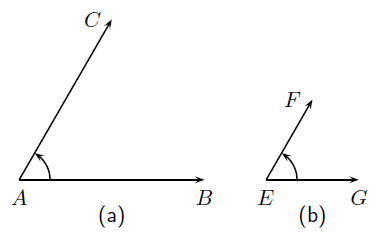
\includegraphics{
% col11306.imgs/m39370_MG10C13_003.png} % m39370;MG10C13\_003.png;;;6.0;8.5;
% \vspace{2pt}
% \vspace{\rubberspace}\par \begin{cnxcaption}
% \small \textbf{Figure 12.3: }Examples of angles. $\hat{A}=\hat{E}$, even though
% the lines making up the angles are of different lengths.
% \end{cnxcaption}
% \vspace{.1in}
% \rule[.1in]{\figurerulewidth}{.005in} \\
% \end{center}
% \end{figure}       
% \subsubsection{ Measuring angles}
% \nopagebreak
% The size of an angle does not depend on the length of the lines that are joined
% to make up the angle, but depends only on how both the lines are placed as can
% be seen in Figure~12.3. This means that the idea of length cannot be used to
% measure angles. An angle is a rotation around the vertex.\par 
% 
% \subsubsection{ Using a Protractor}
% \nopagebreak
% A protractor is a simple tool that is used to measure angles. A picture of a
% protractor is shown in Figure~12.4.\par 
% \setcounter{subfigure}{0}
% \begin{figure}[H] % horizontal\label{m39370*uid13}
% \begin{center}
% \rule[.1in]{\figurerulewidth}{.005in} \\
% \label{m39370*uid13!!!underscore!!!media}\label{
% m39370*uid13!!!underscore!!!printimage}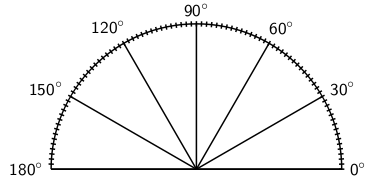
\includegraphics{
% col11306.imgs/m39370_MG10C13_004.png} % m39370;MG10C13\_004.png;;;6.0;8.5;
% \vspace{2pt}
% \vspace{\rubberspace}\par \begin{cnxcaption}
% \small \textbf{Figure 12.4: }Diagram of a protractor.
% \end{cnxcaption}
% \vspace{.1in}
% \rule[.1in]{\figurerulewidth}{.005in} \\
% \end{center}
% \end{figure}       
% 
% \textbf{Method:}
% \par 
% Using a protractor\par 
% \begin{enumerate}[noitemsep, label=\textbf{\arabic*}. ] 
% \item Place the bottom line of the protractor along one line of the angle so
% that the other line of the angle points at the degree markings.
% \item Move the protractor along the line so that the centre point on the
% protractor is at the vertex of the two lines that make up the angle.
% \item Follow the second line until it meets the marking on the protractor and
% read off the angle. Make sure you start measuring at 0$^{\circ }$.
% \end{enumerate}
% 
% \subsubsection{  Measuring Angles : Use a protractor to measure the following
% angles:}
% 
% 
% \setcounter{subfigure}{0}
% \begin{figure}[H] % horizontal\label{m39370*id314484}
% \begin{center}
% \label{m39370*id314484!!!underscore!!!media}\label{
% m39370*id314484!!!underscore!!!printimage}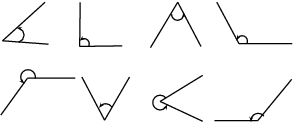
\includegraphics{
% col11306.imgs/m39370_MG10C13_005.png} % m39370;MG10C13\_005.png;;;6.0;8.5;
% \vspace{2pt}
% \vspace{.1in}
% \end{center}
% \end{figure}       
% \par 
% 
% \subsubsection{ Special Angles}
% \nopagebreak
% What is the smallest angle that can be drawn? The figure below shows two lines
% ($CA$ and $AB$) making an angle at a common vertex $A$. If line $CA$ is rotated
% around the common vertex $A$, down towards line $AB$, then the smallest angle
% that can be drawn occurs when the two lines are pointing in the same direction.
% This gives an angle of 0$^{\circ }$. This is shown in Figure~12.6\par 
% 
% \setcounter{subfigure}{0}
% \begin{figure}[H] % horizontal\label{m39370*id314593}
% \begin{center}
% \label{m39370*id314593!!!underscore!!!media}\label{
% m39370*id314593!!!underscore!!!printimage}\includegraphics[width=.8\columnwidth]
% {col11306.imgs/m39370_MG10C13_006.png} % m39370;MG10C13\_006.png;;;6.0;8.5;
% \vspace{2pt}
% \vspace{.1in}
% \end{center}
% \end{figure}       
% \par 
% If line $CA$ is now swung upwards, any other angle can be obtained. If line $CA$
% and line $AB$ point in opposite directions (the third case in Figure~12.6) then
% this forms an angle of 180$^{\circ }$.\par 
% 
% \Tip{If three points $A$, $B$ and $C$ lie on a straight line, then the angle
% between them is 180$^{\circ }$. Conversely, if the angle between three points is
% 180$^{\circ }$, then the points lie on a straight line.}
% 
% \par
% An angle of 90$^{\circ }$ is called a right angle. A right angle is half the
% size of the angle made by a straight line (180$^{\circ }$). We say $CA$ is
% perpendicular to $AB$ or $CA\perp AB$. An angle twice the size of a straight
% line is 360$^{\circ }$. An angle measuring 360$^{\circ }$ looks identical to an
% angle of 0$^{\circ }$, except for the labelling. We call this a revolution.\par 
% \setcounter{subfigure}{0}
% \begin{figure}[H] % horizontal\label{m39370*uid18}
% \begin{center}
% \rule[.1in]{\figurerulewidth}{.005in} \\
% \label{m39370*uid18!!!underscore!!!media}\label{
% m39370*uid18!!!underscore!!!printimage}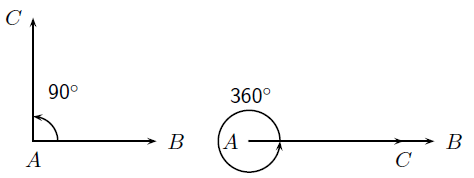
\includegraphics[width=.8\columnwidth]{
% col11306.imgs/m39370_MG10C13_007.png} % m39370;MG10C13\_007.png;;;6.0;8.5;
% \vspace{2pt}
% \vspace{\rubberspace}\par \begin{cnxcaption}
% \small \textbf{Figure 12.7: }An angle of 90$^{\circ }$ is known as a right
% angle.
% \end{cnxcaption}
% \vspace{.1in}
% \rule[.1in]{\figurerulewidth}{.005in} \\
% \end{center}
% \end{figure}       
% 
% \subsubsection{  Angles larger than 360$^{\circ }$ }
% \nopagebreak
% All angles larger than 360$^{\circ }$ also look like we have seen them before.
% If you are given an angle that is larger than 360$^{\circ }$, continue
% subtracting 360$^{\circ }$ from the angle, until you get an answer that is
% between 0$^{\circ }$and 360$^{\circ }$. Angles that measure more than
% 360$^{\circ }$ are largely for mathematical convenience. \par 
% 
% \Tip{
% \begin{itemize}[noitemsep]
% \item Acute angle: An angle $\ge {0}^{\circ }$ and $<{90}^{\circ }$.
% \item Right angle: An angle measuring ${90}^{\circ }$.
% \item Obtuse angle: An angle $>{90}^{\circ }$ and $<{180}^{\circ }$.
% \item Straight angle: An angle measuring 180$^{\circ }$.
% \item Reflex angle: An angle $>{180}^{\circ }$ and $<{360}^{\circ }$.
% \item Revolution: An angle measuring ${360}^{\circ }$.
% \end{itemize}
% These are simply labels for angles in particular ranges, shown in Figure~12.8.}
% \par
% \setcounter{subfigure}{0}
% \begin{figure}[H] % horizontal\label{m39370*uid25}
% \begin{center}
% \rule[.1in]{\figurerulewidth}{.005in} \\
% \label{m39370*uid25!!!underscore!!!media}\label{
% m39370*uid25!!!underscore!!!printimage}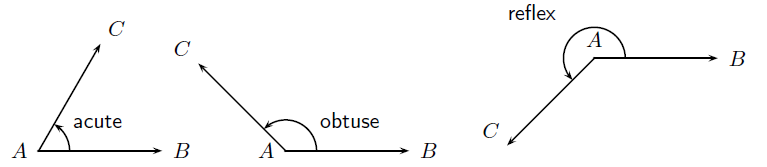
\includegraphics[width=.8\columnwidth]{
% col11306.imgs/m39370_MG10C13_008.png} % m39370;MG10C13\_008.png;;;6.0;8.5;
% \vspace{2pt}
% \vspace{\rubberspace}\par \begin{cnxcaption}
% \small \textbf{Figure 12.8: }Three types of angles defined according to their
% ranges.
% \end{cnxcaption}
% \vspace{.1in}
% \rule[.1in]{\figurerulewidth}{.005in} \\
% \end{center}
% \end{figure}       
% Once angles can be measured, they can then be compared. For example, all right
% angles are 90$^{\circ }$, therefore all right angles are equal and an obtuse
% angle will always be larger than an acute angle.\par The following video
% summarizes what you have learnt so far about angles.
% \setcounter{subfigure}{0}
% \begin{figure}[H] % horizontal\label{m39370*angles-1}
% \textnormal{Khan Academy video on angles - 1}\vspace{.1in} \nopagebreak
% \label{m39370*yt-media1}\label{m39370*yt-video1}
% \raisebox{-5 pt}{ 
\includegraphics[width=0.5cm]{col11306.imgs/summary_www.png}}
% { (Video:  MG10088 )}
% \vspace{2pt}
% \vspace{.1in}
% \end{figure}       
% Note that for high school trigonometry you will be using degrees, not radians as
% stated in the video. \par 

\subsection*{Properties and notation}
\nopagebreak
In the diagram below, the two straight lines $AB$ and $CD$ intersect at point X, forming the four
angles $\hat{A}$, $\hat{B}$, $\hat{C}$ and $\hat{D}$.\par 
% Need new diagram here 
\setcounter{subfigure}{0}
 	\begin{figure}[H] 
    \begin{center}
\scalebox{.8}{
\begin{pspicture}(-0.5,-0.5)(5,2)
%\psgrid
\psset{xunit=0.7cm,yunit=0.6cm}
\SpecialCoor
\psline[arrows=<->](0,0)(6,3)
\psline[arrows=<->](0,3)(6,0)
\psdot[dotsize=1pt](3,1.5)
% \uput[l](0,0){$A$}
% \uput[r](6,3){$B$}
% \uput[l](0,3){$C$}
% \uput[r](6,0){$D$}
% \uput[u](3,1.5){$X$}
\psarc(3,1.5){0.4}{330}{30}
\psarc(3,1.5){0.4}{150}{210}
\psarc(3,1.5){0.5}{30}{150}
\psarc(3,1.5){0.5}{210}{330}
\psarc(3,1.5){0.6}{30}{150}
\psarc(3,1.5){0.6}{210}{330}
\rput(3,1.5){
\uput[r](0.5;0){$\hat{A}$}
\uput[u](0.6;90){$\hat{B}$}
\uput[l](0.5;180){$\hat{C}$}
\uput[d](0.6;270){$\hat{D}$}
}
\end{pspicture}
}
    \end{center}
% \caption{Two intersecting straight lines with vertical angles $\hat{A},\hat{C}$ and $\hat{B},\hat{D}$.}
\label{fig:mg:f:specialangles2}
 \end{figure}        
The table summarises the special angle pairs that result.\par 
% \textbf{m39370*id315548}\par
\begin{table}[H]
\begin{center}
\begin{tabular}{|l|p{4cm}|l|} \hline
Term & Property & Example\\ \hline
Acute angle & $0^{\circ} \leq \mbox{angle} \leq 90^{\circ}$ & $\hat{A}$; $\hat{C}$ \\ \hline
Right angle & Angle $= 90^{\circ}$ &  \\ \hline
Obtuse angle & $90^{\circ} \leq \mbox{angle} \leq 180^{\circ}$ & $\hat{B}$; $\hat{D}$ \\ \hline
Straight angle & Angle $= 180^{\circ}$ & $\hat{A} + \hat{B}$\\
& & $\hat{B} + \hat{C}$ etc.  \\ \hline
Reflex angle & $180^{\circ} < \mbox{angle} < 180^{\circ}$ &  \\ \hline
Adjacent angles & Angles that share a common vertex and a common side. & $\hat{A}$ and $\hat{D}$ \\ 
& & $\hat{C}$ and $\hat{D}$ etc. \\ \hline
Vertically opposite angles & Angles opposite each other when two lines intersect. They share a vertex and are equal. & $\hat{A}=\hat{C}$\\
 &  & $\hat{B}=\hat{D}$\\ \hline
Supplementary angles & Angles that add up to $180^{\circ}$ & $\hat{A}+\hat{B}=180^{\circ}$\\ \hline
& & $\hat{B}+\hat{C}=180^{\circ}$ etc. \\ \hline
Complentary angles & Angles that add up to $90^{\circ}$ & \\ \hline
Revolution & The sum of all angles round a point &  $\hat{A}+\hat{B}+\hat{C}+\hat{D}=360^{\circ}$ \\ \hline

\end{tabular}
\end{center}
\end{table}
\par

\Note{Adjacent angles on a straight line are supplementary.
}
The following video summarises what you have learnt so far
\setcounter{subfigure}{0}
\begin{figure}[H] % horizontal\label{m39370*angles-2}
\textnormal{Khan Academy video on angles - 2}\vspace{.1in} \nopagebreak
\label{m39370*yt-media2}\label{m39370*yt-video2}
\raisebox{-5 pt}{ 
\includegraphics[width=0.5cm]{col11306.imgs/summary_www.png}}
{ (Video:  MG10089 )}
\vspace{2pt}
\vspace{.1in}
\end{figure}       \par 

\subsubsection{Parallel lines and transversal lines}
Two lines intersect if they cross each other at a point. For example, at a
traffic intersection two or more streets intersect; the middle of the
intersection is the common point between the streets.\par 
Parallel lines are always the same distant apart and they are denoted by arrow symbols as shown below. \par 

\setcounter{subfigure}{0}
\begin{figure}[H]
 \begin{center}
\scalebox{1}{
  \begin{pspicture}(0,0)(5,5)
%Lines MN and OP
\psline[linewidth=0.04cm](0,0)(5,3)
\psline[linewidth=0.01cm,arrowsize=0.2cm 2.0,arrowlength=1.4,arrowinset=0.5]{->}(2.3,1.4)(2.7,1.6)
\psline[linewidth=0.04cm](0.5,-.5)(5.5,2.5)
\psline[linewidth=0.01cm,arrowsize=0.2cm 2.0,arrowlength=1.4,arrowinset=0.5]{->}(2.5,0.7)(2.8,.9)
%Lines AB and CD
\psline[linewidth=0.04cm](2.5,-.5)(0.5,2.5)
\psline[linewidth=0.01cm,arrowsize=0.2cm 2.0,arrowlength=1.4,arrowinset=0.5]{->>}(2.5,-0.5)(2.2,0)
\psline[linewidth=0.04cm](5,0)(3,3)
\psline[linewidth=0.01cm,arrowsize=0.2cm 2.0,arrowlength=1.4,arrowinset=0.5]{->>}(4.6,0.6)(4.3,1.1)
%And the labels
\rput[t](0.5,2.8){M}
\rput[b](2.5,-.8){N}
\rput[b](5,-.3){P}
\rput[t](3,3.3){O}
\rput[l](-.3,0){A}
\rput[r](5.3,3){B}
\rput[l](0.2,-.5){C}
\rput[r](5.8,2.5){D}
  \end{pspicture}
}
$AB \parallel CD$ and $MN \parallel OP$  
 \end{center}
\end{figure} 
    
\par 
\Note{
A section of the Australian National Railways Trans-Australian line is perhaps
one of the longest pairs of man-made parallel lines.
The Australian National Railways Trans-Australian line over the Nullarbor Plain,
is 478~km (297 miles) dead straight, from Mile 496, between Nurina and Loongana,
Western Australia, to Mile 793, between Ooldea and Watson, South
Australia.(Source: www.guinnessworldrecords.com)} % end \textsl

A transversal line intersects two or more parallel lines. In the diagram below, $AB \parallel CD$ and $EF$ is a
transversal. The properties of the angles formed by these intersecting lines are summarised in the table below.\par 
\setcounter{subfigure}{0}
\begin{figure}[htb]
\begin{center}
\begin{pspicture}(0,-1.5)(6,3.5)
%\psgrid[gridcolor=lightgray]
\psline{-}(0,0)(6,0)
\psline[arrows=->>](0,0)(1.5,0)
\uput[l](0,0){$A$}
\uput[r](6,0){$B$}
\psline{-}(0,2)(6,2)
\psline[arrows=->>](0,2)(1.5,2)
\uput[l](0,2){$C$}
\uput[r](6,2){$D$}
\psline{-}(1,-1)(5,3)
\uput[dl](1,-1){$E$}
\uput[ur](5,3){$F$}

\psarc(4,2){0.5}{0}{45} \uput{0.6}[22.5](4,2){$g$}
\psarc(4,2){0.3}{45}{180} \psarc(4,2){0.4}{45}{180} \uput{0.5}[112.5](4,2){$h$}
\psarc(4,2){0.5}{180}{225} \uput{0.6}[202.5](4,2){$a$}
\psarc(4,2){0.3}{225}{360} \psarc(4,2){0.4}{225}{360} \uput{0.5}[292.5](4,2){$b$}
\psarc(2,0){0.5}{0}{45} \uput{0.6}[22.5](2,0){$c$}
\psarc(2,0){0.3}{45}{180} \psarc(2,0){0.4}{45}{180} \uput{0.5}[112.5](2,0){$d$}
\psarc(2,0){0.5}{180}{225} \uput{0.6}[202.5](2,0){$e$}
\psarc(2,0){0.3}{225}{360} \psarc(2,0){0.4}{225}{360} \uput{0.5}[292.5](2,0){$f$}
\end{pspicture}
% \caption{Parallel lines intersected by a transversal}
\label{fig:mg:f:partrans}
\end{center}
\end{figure}      
% \textbf{m39370*uid30}\par
\begin{table}[H]
\begin{center}
%\caption{Properties of angles formed when parallel lines are intersected by a transversal. The example in Figure~\ref{fig:mg:f:partrans} is used as a reference.}
\label{tab:mg:f:partrans}
\begin{tabular}{|p{3cm}|p{3cm}|p{3cm}|m{3cm}|}\hline
\textbf{Name of angle} & \textbf{Definition} & \textbf{Examples} & \textbf{Notes}\\\hline\hline
interior angles & angles that lie inside the parallel lines & $a$, $b$, $c$ and $d$ are interior angles & interior means inside \\ \hline
exterior angles & angles that lie outside the parallel lines & $e$, $f$, $g$ and $h$ are exterior angles & exterior means outside \\ \hline
corresponding angles & equal angles on the same side of the parallel lines and the same side of the transversal & $\hat{a} = \hat{e}$  $\hat{b} = \hat{f}$,  $\hat{c} = \hat{g}$ and  $\hat{d} = \hat{h}$ are corresponding angles. &
%\scalebox{1} % Change this value to rescale the drawing.
% \begin{center}
%{
\begin{pspicture}(0,-0.9846875)(1.48,0.7846875)
\psline[linewidth=0.04cm](0.2,0.7646875)(1.46,0.7646875)
\psline[linewidth=0.04cm](0.22,0.1246875)(1.44,0.1246875)
\psline[linewidth=0.04cm,arrowsize=0.05291667cm 2.0,arrowlength=1.4,arrowinset=0.4]{->>}(0.38,0.1246875)(1.16,0.1246875)
\psline[linewidth=0.04cm,arrowsize=0.05291667cm 2.0,arrowlength=1.4,arrowinset=0.4]{->>}(0.22,0.7646875)(1.0,0.7646875)
%\usefont{T1}{ptm}{m}{n}
\rput(0.7209375,-0.7653125){F shape}
\psline[linewidth=0.04cm](0.2,0.7646875)(0.2,-0.5353125)
\psarc[linewidth=0.04](0.2,0.7446875){0.2}{270.0}{351.8699}
\psarc[linewidth=0.04](0.22,0.1046875){0.2}{270.0}{351.8699}
\end{pspicture}
%}
% \end{center}
\\\hline
 co-interior angles on the same side &  co-interior equal angles that lie inside the parallel lines and on the same side of the transversal &  $\hat{a} + \hat{d} = 180^{\circ}$, $\hat{b} + \hat{c} = 180^{\circ}$&
% \begin{center}
%\scalebox{1} % Change this value to rescale the drawing.
%{
\begin{pspicture}(0,-0.8346875)(1.6,0.6346875)
\psline[linewidth=0.04cm](0.2,0.6146875)(1.46,0.6146875)
\psline[linewidth=0.04cm](0.22,-0.3453125)(1.58,-0.3453125)
\psline[linewidth=0.04cm,arrowsize=0.05291667cm 2.0,arrowlength=1.4,arrowinset=0.4]{->>}(0.38,-0.3453125)(1.16,-0.3453125)
\psline[linewidth=0.04cm,arrowsize=0.05291667cm 2.0,arrowlength=1.4,arrowinset=0.4]{->>}(0.22,0.6146875)(1.0,0.6146875)
\psarc[linewidth=0.04](0.2,-0.2653125){0.2}{329.03625}{90.0}
%\usefont{T1}{ptm}{m}{n}
\rput(0.8084375,-0.6153125){C shape}
\psline[linewidth=0.04cm](0.2,0.6146875)(0.2,-0.3653125)
\psarc[linewidth=0.04](0.2,0.5946875){0.2}{270.0}{351.8699}
\end{pspicture}
%}
% \end{center}
\\\hline
 alternate interior angles & equal interior angles that lie inside the parallel line and on opposite sides of the transversal & $\hat{a} = \hat{c}$, $\hat{b} = \hat{d}$ &
% \begin{center}
%\scalebox{1} % Change this value to rescale the drawing.
%{
\begin{pspicture}(0,-0.8246875)(1.4434375,0.6446875)
\psline[linewidth=0.04cm](0.0434375,0.6246875)(1.3034375,0.6246875)
\psline[linewidth=0.04cm](1.3034375,0.6246875)(0.0634375,-0.3353125)
\psline[linewidth=0.04cm](0.0634375,-0.3353125)(1.4234375,-0.3353125)
\psline[linewidth=0.04cm,arrowsize=0.05291667cm 2.0,arrowlength=1.4,arrowinset=0.4]{->>}(0.2234375,-0.3353125)(1.0034375,-0.3353125)
\psline[linewidth=0.04cm,arrowsize=0.05291667cm 2.0,arrowlength=1.4,arrowinset=0.4]{->>}(0.0634375,0.6246875)(0.8434375,0.6246875)
\psarc[linewidth=0.04](1.2034374,0.5846875){0.2}{168.69006}{243.43495}
\psarc[linewidth=0.04](0.2034375,-0.2353125){0.2}{329.03625}{45.0}
%\usefont{T1}{ptm}{m}{n}
\rput(0.6428125,-0.6053125){Z shape}
\end{pspicture}
%}
% \end{center}
\\\hline
\end{tabular}
\end{center}
\end{table}
If two lines are intersected by a transversal such that:
\begin{itemize}[noitemsep]
 \item corresponding angles are equal \newline \textbf{or}
\item alternate interior angles are equal \newline \textbf{or}
\item co-interior angles are supplementary
\end{itemize}
then the two lines are parallel.
	\begin{figure}[H] % horizontal\label{m38380*angles-3}    
    \textnormal{Khan Academy video on angles - 3}\vspace{.1in} \nopagebreak
  \label{m38380*yt-media3}\label{m38380*yt-video3}
            \raisebox{-5 pt}{

\includegraphics[width=0.5cm]{col11306.imgs/summary_www.png}} { (Video:  P10116
)}
      \vspace{2pt}
    \vspace{.1in}
 \end{figure} 

% \begin{wex}{Finding angles}
% {Find all the unknown angles. Is $EF \parallel CG$? Explain your answer.
%  \begin{center}
%    \scalebox{0.8} % Change this value to rescale the drawing.
% {
% \begin{pspicture}(0,-2.381875)(11.965313,2.381875)
% \psline[linewidth=0.04cm,arrowsize=0.05291667cm 4.0,arrowlength=1.4,arrowinset=0.64]{->>}(3.68,0.2634375)(4.32,0.6234375)
% \psline[linewidth=0.04cm,arrowsize=0.05291667cm 4.0,arrowlength=1.4,arrowinset=0.64]{->>}(8.18,0.0034375)(8.8,0.3634375)
% \rput{-138.03267}(7.6911535,4.7037997){\psarc[linewidth=0.04](4.7476172,0.87697935){0.42959735}{343.58032}{85.22324}}
% \psline[linewidth=0.04cm](0.0,-1.9565625)(6.62,2.0234375)
% \psline[linewidth=0.04cm](4.96,-1.9365625)(11.58,2.0434375)
% \psline[linewidth=0.04cm](2.96,-1.9165626)(9.0,-1.9165626)
% \psline[linewidth=0.04cm](4.96,-1.9165626)(5.0,1.0834374)
% \psline[linewidth=0.04cm](2.44,-0.4565625)(11.62,1.5634375)
% \psline[linewidth=0.04cm](4.8,-1.8965625)(4.8,-1.7765625)
% \psline[linewidth=0.04cm](4.78,-1.7565625)(4.98,-1.7565625)
% \usefont{T1}{ptm}{m}{n}
% \rput(4.813594,0.7184375){\footnotesize $60^{\circ}$}
% \psbezier[linewidth=0.04](1.92,-0.7965625)(2.4652674,-1.0965625)(3.0,-0.60322917)(2.98,-0.3365625)
% \usefont{T1}{ptm}{m}{n}
% \rput{30.259655}(-0.014254112,-1.339781){\rput(2.4535937,-0.6815625){\footnotesize $160^{\circ}$}}
% \psarc[linewidth=0.04](5.09,-1.5865625){0.39}{351.02737}{104.74356}
% \rput{-33.527527}(1.8911341,2.8561378){\psarc[linewidth=0.04](5.6863933,-1.7109741){0.33947578}{0.0}{99.46232}}
% \rput{-210.4531}(18.081177,-3.2094462){\psarc[linewidth=0.04](9.477381,0.85604936){0.3534083}{0.0}{75.4531}}
% \rput{-28.674759}(0.5472108,5.594595){\psarc[linewidth=0.04](11.218004,1.7268189){0.32564545}{343.67474}{75.4531}}
% \psbezier[linewidth=0.04](9.76,0.9748661)(10.232,0.5634375)(10.94,1.1120089)(10.808888,1.3634375)
% \usefont{T1}{ptm}{m}{n}
% \rput(5.2014065,-1.4865625){$x$}
% \usefont{T1}{ptm}{m}{n}
% \rput(5.6914062,-1.7065625){$s$}
% \usefont{T1}{ptm}{m}{n}
% \rput(9.4114065,0.9334375){$y$}
% \usefont{T1}{ptm}{m}{n}
% \rput(10.361406,1.0534375){$r$}
% \usefont{T1}{ptm}{m}{n}
% \rput(11.211407,1.6534375){$p$}
% \usefont{T1}{ptm}{m}{n}
% \rput(4.8871875,-2.2265625){C}
% \usefont{T1}{ptm}{m}{n}
% \rput(9.201094,-2.0865624){G}
% \usefont{T1}{ptm}{m}{n}
% \rput(11.76,2.2134376){D}
% \usefont{T1}{ptm}{m}{n}
% \rput(11.829687,1.5134375){F}
% \usefont{T1}{ptm}{m}{n}
% \rput(0.1865625,-2.1465626){A}
% \usefont{T1}{ptm}{m}{n}
% \rput(2.3420312,-0.1665625){E}
% \usefont{T1}{ptm}{m}{n}
% \rput(4.8671875,1.3734375){B}
% \end{pspicture} 
% }
%  \end{center}
% } 
% {\westep{Step 1:}
% \westep{Step 2:}
% \westep{Step 3:}
% }
% \end{wex}

  \label{m38380*secfhsst!!!underscore!!!id550}
\begin{exercises}{Angles}
        \nopagebreak
        \label{m38380*eip-407}\begin{enumerate}[noitemsep,
label=\textbf{\arabic*}. ] 
            \item Use adjacent, corresponding, co-interior and alternate angles
to fill in all the angles labeled with letters in the diagram below:

\begin{pspicture}(0,-1.7981373)(6.5116725,1.7981373)
\psline[linewidth=0.04cm](0.34542254,0.6181373)(5.2654223,0.6181373)
\psline[linewidth=0.04cm](0.34542254,-0.7418627)(5.2654223,-0.7418627)
\psline[linewidth=0.04cm](0.0,-1.7781373)(5.5254226,1.7781373)
\usefont{T1}{ptm}{m}{n}
\rput(5.1533914,0.9881373){42$^\circ$}
\usefont{T1}{ptm}{m}{n}
\rput(3.664485,0.8881373){a}
\usefont{T1}{ptm}{m}{n}
\rput(3.0458913,0.3881373){b}
\usefont{T1}{ptm}{m}{n}
\rput(3.8072975,0.4081373){c}
\usefont{T1}{ptm}{m}{n}
\rput(1.5262038,-0.5518627){d}
\usefont{T1}{ptm}{m}{n}
\rput(2.2315164,-0.5518627){e}
\usefont{T1}{ptm}{m}{n}
\rput(1.6212038,-1.0518627){f}
\usefont{T1}{ptm}{m}{n}
\rput(0.7930787,-0.9118627){g}
\rput{-66.70425}(1.9155159,4.522671){\psarc[linewidth=0.032,arrowsize=0.05291667cm 2.0,arrowlength=1.4,arrowinset=0.4]{->}(4.3934965,0.8061751){0.24084859}{20.012312}{156.69316}}
\psline[linewidth=0.04](3.9254224,-0.6018627)(4.2254224,-0.7418627)(3.9454224,-0.8818627)
\psline[linewidth=0.04](3.6854224,-0.6018627)(3.9854226,-0.7418627)(3.7054226,-0.8818627)
\psline[linewidth=0.04](2.2454226,0.7581373)(2.5454226,0.6181373)(2.2654226,0.47813728)
\psline[linewidth=0.04](2.0054226,0.7581373)(2.3054225,0.6181373)(2.0254226,0.47813728)
\end{pspicture}

            \item Find all the unknown angles in the figure below:
\scalebox{1.3} {
\begin{pspicture}(0,-1.6504478)(5.097969,1.7279896)
\psline[linewidth=0.04cm](2.8765626,1.4495522)(4.8165627,-1.4104478)
\psline[linewidth=0.04cm](0.2365625,1.2295521)(2.1765625,-1.6304479)
\psline[linewidth=0.04cm,arrowsize=0.1cm 3.0,arrowlength=1.4,arrowinset=0.4]{->>}(0.26,1.1879896)(1.1165625,-0.07044793)
\psline[linewidth=0.04cm,arrowsize=0.1cm 3.0,arrowlength=1.4,arrowinset=0.4]{->>}(3.0765624,1.1495521)(4.06,-0.25201043)
\psline[linewidth=0.04cm](1.2765625,-0.29044786)(4.2165623,-0.51044786)
\psline[linewidth=0.04cm](0.6365625,0.66955215)(3.5765624,0.44955212)
\psline[linewidth=0.04cm,arrowsize=0.08cm 2.5,arrowlength=1.4,arrowinset=0.4]{->}(1.2965626,-0.29044792)(2.8965626,-0.43044794)
\psline[linewidth=0.04cm,arrowsize=0.08cm 2.5,arrowlength=1.4,arrowinset=0.4]{->}(0.7765625,0.6695522)(2.54,0.52798957)
\psline[linewidth=0.04cm](3.5365624,0.44955212)(1.2765625,-0.29044786)
\psline[linewidth=0.04cm](4.1765623,-0.51044786)(1.9165626,-1.2504479)
\psline[linewidth=0.04cm,arrowsize=0.08cm 2.5,arrowlength=1.4,arrowinset=0.4]{->}(2.9765625,0.26955208)(2.1365626,-0.05044793)
\psline[linewidth=0.04cm,arrowsize=0.08cm 2.5,arrowlength=1.4,arrowinset=0.4]{->}(3.1765625,0.34955207)(2.3365624,0.029552069)
\psline[linewidth=0.04cm,arrowsize=0.08cm 2.5,arrowlength=1.4,arrowinset=0.4]{->}(3.3965626,0.42955208)(2.5565624,0.10955207)
\psline[linewidth=0.04cm,arrowsize=0.08cm 2.5,arrowlength=1.4,arrowinset=0.4]{->}(3.5165625,-0.73044795)(2.66,-1.0320104)
\psline[linewidth=0.04cm,arrowsize=0.08cm 2.5,arrowlength=1.4,arrowinset=0.4]{->}(3.7165625,-0.6504479)(2.8765626,-0.97044796)
\psline[linewidth=0.04cm,arrowsize=0.08cm 2.5,arrowlength=1.4,arrowinset=0.4]{->}(3.9365625,-0.5704479)(3.0965624,-0.8904479)
\usefont{T1}{ptm}{m}{n}
\rput(0.12375,1.2395521){A}
\usefont{T1}{ptm}{m}{n}
\rput(0.403125,0.55955213){B}
\usefont{T1}{ptm}{m}{n}
\rput(0.4890625,-0.58044785){C}
\usefont{T1}{ptm}{m}{n}
\rput(1.7354687,-1.3404479){D}
\usefont{T1}{ptm}{m}{n}
\rput(3.0051563,1.5595521){E}
\usefont{T1}{ptm}{m}{n}
\rput(3.7190626,0.5395521){F}
\usefont{T1}{ptm}{m}{n}
\rput(4.3729687,-0.4204479){G}
\usefont{T1}{ptm}{m}{n}
\rput(4.928594,-1.2804478){H}
\usefont{T1}{ptm}{m}{n}
\rput(1.3218751,0.41455212){\scriptsize 70$^\circ$}
\usefont{T1}{ptm}{m}{n}
\rput(2.1242187,-0.8654478){\scriptsize 80$^\circ$}
\usefont{T1}{ptm}{m}{n}
\rput(0.6675,0.79955214){\tiny 1}
\usefont{T1}{ptm}{m}{n}
\rput(3.2075,0.6595521){\tiny 1}
\usefont{T1}{ptm}{m}{n}
\rput(2.9325001,0.37955213){\tiny 2}
\usefont{T1}{ptm}{m}{n}
\rput(3.4242187,0.25955212){\tiny 3}
\usefont{T1}{ptm}{m}{n}
\rput(3.9075,-0.40044788){\tiny 1}
\usefont{T1}{ptm}{m}{n}
\rput(3.5325,-0.6204479){\tiny 2}
\usefont{T1}{ptm}{m}{n}
\rput(4.084219,-0.70044786){\tiny 3}
\usefont{T1}{ptm}{m}{n}
\rput(1.3275001,-0.08044788){\tiny 1}
\usefont{T1}{ptm}{m}{n}
\rput(1.9325,-0.24044788){\tiny 2}
\usefont{T1}{ptm}{m}{n}
\rput(1.5842187,-0.52044785){\tiny 3}
\usefont{T1}{ptm}{m}{n}
\rput(2.1075,-1.3204479){\tiny 1}
\rput{-165.35927}(1.3568144,1.2702812){\psarc[linewidth=0.04](0.76,0.54798955){0.28}{104.03625}{180.0}}
\rput{-45.10457}(1.503625,1.0367023){\psarc[linewidth=0.04](2.0,-1.2920104){0.28}{71.09586}{180.0}}
\end{pspicture} 
}   
 \item Find the value of $x$ in the figure below:
\scalebox{1.3} 
{
\begin{pspicture}(0,-2.1645312)(2.9317186,2.1645312)
\psline[linewidth=0.04cm](0.4409375,1.8007812)(0.4409375,-1.7392187)
\psline[linewidth=0.04cm](1.4409375,1.8007812)(1.4409375,-1.7392187)
\psline[linewidth=0.04cm](0.2009375,1.0007813)(2.28,-0.91546875)
\psline[linewidth=0.04cm](1.6809375,0.18078125)(0.2809375,-1.6992188)
\usefont{T1}{ptm}{m}{n}
\rput(0.468125,1.9907813){A}
\usefont{T1}{ptm}{m}{n}
\rput(0.4275,-2.0092187){B}
\usefont{T1}{ptm}{m}{n}
\rput(1.4334375,-2.0092187){C}
\usefont{T1}{ptm}{m}{n}
\rput(1.4398437,1.9907813){D}
\usefont{T1}{ptm}{m}{n}
\rput(0.1240625,0.67078125){X}
\usefont{T1}{ptm}{m}{n}
\rput(1.3248438,-0.58921874){Y}
\usefont{T1}{ptm}{m}{n}
\rput(0.245625,-1.3892188){Z}
\psline[linewidth=0.04cm](0.4209375,1.4407812)(0.5409375,1.6807812)
\psline[linewidth=0.04cm](0.4209375,1.5007813)(0.3409375,1.6807812)
\psline[linewidth=0.04cm](1.4409375,1.5407813)(1.5409375,1.7207812)
\psline[linewidth=0.04cm](1.4409375,1.5407813)(1.3409375,1.7007812)
\usefont{T1}{ptm}{m}{n}
\rput(0.62671876,0.32578126){\scriptsize 4$x$}
\usefont{T1}{ptm}{m}{n}
\rput(1.6839062,-0.11421875){\scriptsize $x$}
\usefont{T1}{ptm}{m}{n}
\rput(1.9114062,-0.99421877){\scriptsize $x$+20$^\circ$}
\rput{-178.50352}(3.0830076,-0.7128394){\psarc[linewidth=0.04](1.536849,-0.3765517){0.17893833}{61.938473}{168.11142}}
\end{pspicture} 
} 
 \item  Determine whether there are pairs of parallel lines in the
following figures.
\label{m38380*id79123}\begin{enumerate}[noitemsep, label=\textbf{\alph*}. ] 
            \item 
\scalebox{1} % Change this value to rescale the drawing.
{
\begin{pspicture}(0,-2.451875)(6.3617187,2.451875)
\psline[linewidth=0.04cm](0.0,1.6081251)(6.1,-1.751875)
\psline[linewidth=0.04cm](1.42,2.171875)(1.74,-1.808125)
\psline[linewidth=0.04cm](4.72,2.188125)(5.08,-2.211875)
\usefont{T1}{ptm}{m}{n}
\rput(1.8954687,0.85812503){115$^{\circ}$}
\usefont{T1}{ptm}{m}{n}
\rput(4.583125,-0.621875){55$^{\circ}$}
\usefont{T1}{ptm}{m}{n}
\rput(1.2482814,2.278125){O}
\usefont{T1}{ptm}{m}{n}
\rput(1.5804688,-2.021875){P}
\usefont{T1}{ptm}{m}{n}
\rput(4.9214063,2.178125){Q}
\usefont{T1}{ptm}{m}{n}
\rput(5.2339063,-2.301875){R}
\usefont{T1}{ptm}{m}{n}
\rput(0.1984375,1.678125){S}
\usefont{T1}{ptm}{m}{n}
\rput(6.210781,-1.7818749){T}
\usefont{T1}{ptm}{m}{n}
\rput(1.3671875,0.21812505){A}
\usefont{T1}{ptm}{m}{n}
\rput(4.5465627,-1.361875){B}
\usefont{T1}{ptm}{m}{n}
\rput(1.3509375,0.97812504){\tiny 1}
\usefont{T1}{ptm}{m}{n}
\rput(1.3359375,0.65812504){\tiny 2}
\usefont{T1}{ptm}{m}{n}
\rput(1.6876563,0.51812506){\tiny 3}
\usefont{T1}{ptm}{m}{n}
\rput(5.1876564,-1.5218749){\tiny 3}
\usefont{T1}{ptm}{m}{n}
\rput(5.215937,-1.0618749){\tiny 2}
\usefont{T1}{ptm}{m}{n}
\rput(4.750938,-1.3018749){\tiny 1}
\end{pspicture} 
}
\item 
\scalebox{1} % Change this value to rescale the drawing.
{
\begin{pspicture}(0,-2.8392186)(7.70125,2.8392186)
\psline[linewidth=0.04cm](0.0625,-0.05921875)(7.4625,-0.05921875)
\psline[linewidth=0.04cm](0.6625,-1.9592187)(4.74,2.5192187)
\psline[linewidth=0.04cm](6.1225,2.4007812)(2.0025,-2.6592188)
\usefont{T1}{ptm}{m}{n}
\rput(4.8440623,0.25078127){45$^{\circ}$}
\usefont{T1}{ptm}{m}{n}
\rput(2.5667188,-0.28921875){124$^{\circ}$}
\usefont{T1}{ptm}{m}{n}
\rput(4.7973437,2.6707811){M}
\usefont{T1}{ptm}{m}{n}
\rput(0.601875,-1.7292187){N}
\usefont{T1}{ptm}{m}{n}
\rput(6.250781,2.4707813){O}
\usefont{T1}{ptm}{m}{n}
\rput(2.2229688,-2.6892188){P}
\usefont{T1}{ptm}{m}{n}
\rput(0.10390625,0.19078125){Q}
\usefont{T1}{ptm}{m}{n}
\rput(7.536406,0.13078125){R}
\usefont{T1}{ptm}{m}{n}
\rput(2.21875,0.49078128){K}
\usefont{T1}{ptm}{m}{n}
\rput(4.4520316,-0.5492188){L}
\usefont{T1}{ptm}{m}{n}
\rput(2.3734376,0.13078125){\tiny 1}
\usefont{T1}{ptm}{m}{n}
\rput(2.7584374,0.09078125){\tiny 2}
\usefont{T1}{ptm}{m}{n}
\rput(2.0901563,-0.18921876){\tiny 3}
\usefont{T1}{ptm}{m}{n}
\rput(4.170156,-0.28921875){\tiny 3}
\usefont{T1}{ptm}{m}{n}
\rput(4.0184374,0.09078125){\tiny 2}
\usefont{T1}{ptm}{m}{n}
\rput(3.7334375,-0.22921875){\tiny 1}
\end{pspicture} 
}
    \item 
\scalebox{1} % Change this value to rescale the drawing.
{
\begin{pspicture}(0,-3.1192186)(6.325469,3.1192186)
\psline[linewidth=0.04cm](0.1525,1.0007812)(6.1125,0.98078126)
\psline[linewidth=0.04cm](0.1525,-1.0392187)(6.1125,-1.0192188)
\psline[linewidth=0.04cm](3.0125,3.0007813)(3.3125,-3.0192187)
\usefont{T1}{ptm}{m}{n}
\rput(2.7432813,0.7307812){95$^{\circ}$}
\usefont{T1}{ptm}{m}{n}
\rput(3.6395311,-1.3692188){85$^{\circ}$}
\usefont{T1}{ptm}{m}{n}
\rput(3.24875,2.950781){K}
\usefont{T1}{ptm}{m}{n}
\rput(3.5020313,-2.9692187){L}
\usefont{T1}{ptm}{m}{n}
\rput(0.14734375,-0.88921875){M}
\usefont{T1}{ptm}{m}{n}
\rput(6.0718746,-0.82921875){N}
\usefont{T1}{ptm}{m}{n}
\rput(0.12328125,1.1707813){T}
\usefont{T1}{ptm}{m}{n}
\rput(6.1564064,1.1507812){Y}
\usefont{T1}{ptm}{m}{n}
\rput(3.3034375,0.79078126){\tiny 1}
\usefont{T1}{ptm}{m}{n}
\rput(3.3084376,1.2107813){\tiny 2}
\usefont{T1}{ptm}{m}{n}
\rput(2.9001563,1.1907812){\tiny 3}
\usefont{T1}{ptm}{m}{n}
\rput(3.3234375,-0.88921875){\tiny 1}
\usefont{T1}{ptm}{m}{n}
\rput(2.9884377,-0.88921875){\tiny 2}
\usefont{T1}{ptm}{m}{n}
\rput(3.0201561,-1.2692188){\tiny 3}
\end{pspicture} 
}
    \end{enumerate}
 \item If AB is parallel to CD and AB is parallel to EF, give an explanation why CD must be parallel to EF.
\begin{pspicture}(0,-0.81328124)(3.8328125,0.81328124)
\psline[linewidth=0.04cm](0.2415625,0.6067188)(3.4415624,0.38671875)
\psline[linewidth=0.04cm](0.3015625,-0.09328125)(3.4215624,-0.09328125)
\psline[linewidth=0.04cm](0.3815625,-0.6532813)(3.5215626,-0.55328125)
\rput(0.1221875,-0.10328125){A}
\rput(3.6009376,-0.08328125){B}
\rput(3.654375,-0.5832813){F}
\rput(0.178125,-0.66328126){E}
\rput(0.086875,0.61671877){C}
\rput(3.6504688,0.33671874){D}
\end{pspicture}  
            \end{enumerate}
    \addtocounter{footnote}{-0}
    \par   
\par \raisebox{-5
pt}{
\includegraphics[width=0.5cm]{col11306.imgs/summary_www.png}} Find the
answers with the shortcodes:
 \par \begin{tabular}[h]{cccccc}
 (1.) lxF  &  (2.) lxL  &  (3.) lxM  &  (4.) lxe  &  (5.) lxt  & \end{tabular}
\end{exercises}
        \label{m38380*eip-115}The following video shows some problems with their
solutions

    \setcounter{subfigure}{0}
	\begin{figure}[H] % horizontal\label{m38380*angles-4}
    \textnormal{Khan Academy video on angles - 4}\vspace{.1in} \nopagebreak
  \label{m38380*yt-media4}\label{m38380*yt-video4}
            \raisebox{-5 pt}{

\includegraphics[width=0.5cm]{col11306.imgs/summary_www.png}} { (Video:  P10117
)}
      \vspace{2pt}
    \vspace{.1in}
 \end{figure}  
        \subsection*{Classification of triangles}
        \nopagebreak
        \label{m38380*id317485}A triangle is a three-sided polygon. Triangles can be organised into three categories: equilateral, isoceles and scalene. They can also be categorised according to their angles: acute angled, obtuse angled and right-angled. \par 
\label{m38380*id317683}We use the notation $\Delta ABC$ to
refer to a triangle with corners labeled \begin{math}A\end{math},
\begin{math}B\end{math}, and \begin{math}C\end{math}.\par 
\begin{table}[H]
\begin{center}
\caption{Types of Triangles}
\label{tab:gt:basics:triangles}
\begin{tabular}{|c|m{3.8cm}|m{5cm}|}\hline
Name & Diagram & Properties\\\hline\hline
scalene &
\begin{pspicture}(0,0)(3,1.2)
%\psgrid[gridcolor=lightgray]
\rput(0.35,0){\psset{unit=2}
\pspolygon({1.25;25})({1;0})}
\end{pspicture}
& All sides and angles are different.\\\hline
isosceles &
\begin{pspicture}(-0.40,-0.4)(3.4,3.4)
%\psgrid[gridcolor=lightgray]
\rput(0.7,0){\psset{unit=1.5}
\pstTriangle(0,0){A}(1;0){B}(2;73.4){C}
\pstSegmentMark{B}{C}
\pstSegmentMark{A}{C}
\pstMarkAngle[LabelSep=0.6]{C}{B}{A}{}
\pstMarkAngle[LabelSep=0.6]{B}{A}{C}{}
}
\end{pspicture}
& Two sides are equal in length. The angles opposite the equal sides are equal.\\\hline
equilateral &
\begin{pspicture}(-0.40,-0.4)(3.4,3.2)
%\psgrid[gridcolor=lightgray]
\psset{unit=1.5}
\pstTriangle(0,0){A}(2;0){B}(2;60){C}
\pstSegmentMark{A}{B}
\pstSegmentMark{B}{C}
\pstSegmentMark{A}{C}
\pstMarkAngle[LabelSep=0.6]{A}{C}{B}{$60^{\circ}$}
\pstMarkAngle[LabelSep=0.6]{C}{B}{A}{$60^{\circ}$}
\pstMarkAngle[LabelSep=0.6]{B}{A}{C}{$60^{\circ}$}
\end{pspicture}
& All three sides are equal in length and all three angles are equal.\\\hline
acute & \scalebox{1} % Change this value to rescale the drawing.
{
\begin{pspicture}(0,-1.03)(2.6,1.03)
\psline[linewidth=0.04](0.0,-1.01)(2.06,1.01)(2.58,-0.53)(0.02,-0.99)
\end{pspicture} 
} & All three interior angles are less than $90^{\circ}$ \\ \hline
obtuse & \scalebox{0.8} % Change this value to rescale the drawing.
{
\begin{pspicture}(0,-0.78)(4.7,0.78)
\psline[linewidth=0.04](0.0,-0.76)(4.68,0.76)(3.38,-0.72)(0.02,-0.74)
\end{pspicture} 
} & One interior angle is greater than $180^{\circ}$ \\ \hline
right-angled &
\begin{pspicture}(-0.4,-0.4)(3,3)
%\psgrid[gridcolor=lightgray]
\rput(0.5,0){\psset{unit=2}
\pstTriangle(0,0){A}(1;90){B}(1;0){C}
\pstRightAngle[RightAngleSize=0.2,LabelSep=0.6]{C}{A}{B}
\rput{-45}(0.6,0.6){hypotenuse}}
\end{pspicture}
& one interior angle is $90^{\circ}$\\\hline
\end{tabular}
\end{center}
\end{table}
Different combinations of these properties are also possible. For example, an obtuse isoceles triangle and a right-angled isoceles triangle as shown below.\\
\begin{minipage}{.5\textwidth}
\scalebox{0.6} % Change this value to rescale the drawing.
{
\begin{pspicture}(0,-0.86)(9.98,0.86)
\pspolygon[linewidth=0.04](0.0,0.8)(9.96,0.84)(5.0,-0.84)
\psline[linewidth=0.04cm](2.88,-0.36)(3.14,-0.06)
\psline[linewidth=0.04cm](7.2,0.04)(7.36,-0.18)
\end{pspicture} 
}
\end{minipage}
\begin{minipage}{.5\textwidth}
\scalebox{1} % Change this value to rescale the drawing.
{
\begin{pspicture}(0,-1.07)(2.18,1.07)
\pspolygon[linewidth=0.04](0.14,0.93)(2.16,0.95)(0.12,-1.05)
\psline[linewidth=0.04cm](0.0,0.05)(0.3,0.05)
\psline[linewidth=0.04cm](1.08,1.05)(1.08,0.83)
\psline[linewidth=0.04cm](0.12,0.75)(0.3,0.75)
\psline[linewidth=0.04cm](0.3,0.75)(0.3,0.95)
\end{pspicture} 
}
 \end{minipage}
          
\label{m38380*secfhsst!!!underscore!!!id655}
\begin{Investigation}{Interior angles of a triangle }
        \nopagebreak  
\scalebox{0.8} % Change this value to rescale the drawing.
{
\begin{pspicture}(0,-1.53)(5.96,1.51)
\pstriangle[linewidth=0.04,dimen=outer](3.0,-1.51)(6.0,3.02)
\psline[linewidth=0.04cm,linestyle=dashed,dash=0.16cm 0.16cm](1.5,-0.01)(4.5,-0.01)
\psline[linewidth=0.04cm,linestyle=dashed,dash=0.16cm 0.16cm](3.0,-1.51)(3.0,-0.01)
\usefont{T1}{ptm}{m}{n}
\rput(3.0271876,0.9){A}
\usefont{T1}{ptm}{m}{n}
\rput(0.8665625,-1.2){B}
\usefont{T1}{ptm}{m}{n}
\rput(5.0925,-1.2){C}
\end{pspicture} 
}    
          \label{m38380*id317720}\begin{enumerate}[noitemsep,label=\textbf{\arabic*}. ] 
            \label{m38380*uid41}\item On a piece of paper draw a triangle of any size and shape.
\label{m38380*uid42}\item Cut it out and label the angles.
\begin{math}\hat{A}\end{math}, \begin{math}\hat{B}\end{math} and
\begin{math}\hat{C}\end{math} on both sides of the paper.
\label{m38380*uid43}\item Draw dotted lines as shown and cut along these lines
to get three pieces of paper.
\label{m38380*uid44}\item Place them along your ruler as shown in the figure below.
\item What can we can conclude?
\end{enumerate}
Hint: What is the sum of angles on a straight line?
\scalebox{0.8} % Change this value to rescale the drawing.
{
\begin{pspicture}(0,-2.02)(8.68,2.04)
\usefont{T1}{ptm}{m}{n}
\rput{-134.57147}(6.526203,0.94130903){\rput(3.4573057,-0.9071601){A}}
\usefont{T1}{ptm}{m}{n}
\rput{45.451138}(0.9778306,-3.1181297){\rput(4.2053757,-0.40095752){B}}
\usefont{T1}{ptm}{m}{n}
\rput{-134.99896}(8.521111,1.9342741){\rput(4.648042,-0.8069069){C}}
\psframe[linewidth=0.04,dimen=outer](8.68,-1.22)(0.0,-2.02)
\psline[linewidth=0.04cm](4.78,2.02)(1.66,-1.24)
\psline[linewidth=0.04cm](3.84,-1.2)(3.82,1.04)
\psline[linewidth=0.04cm](7.08,-0.06)(4.78,2.02)
\psline[linewidth=0.04cm](7.04,-0.06)(5.94,-1.22)
\psline[linewidth=0.04cm](5.96,0.96)(3.84,-1.24)
\end{pspicture} 
}
\end{Investigation}

\begin{Investigation}{Exterior angles of a triangle }
        \nopagebreak  
\scalebox{0.8} % Change this value to rescale the drawing.
{
\begin{pspicture}(0,-1.53)(5.96,1.51)
\pstriangle[linewidth=0.04,dimen=outer](3.0,-1.51)(6.0,3.02)
\psline[linewidth=0.04cm,linestyle=dashed,dash=0.16cm 0.16cm](1.5,-0.01)(4.5,-0.01)
\psline[linewidth=0.04cm,linestyle=dashed,dash=0.16cm 0.16cm](3.0,-1.51)(3.0,-0.01)
\usefont{T1}{ptm}{m}{n}
\rput(3.0271876,0.9){A}
\usefont{T1}{ptm}{m}{n}
\rput(0.8665625,-1.2){B}
\usefont{T1}{ptm}{m}{n}
\rput(5.0925,-1.2){C}
\end{pspicture} 
}    
          \label{m38380*id317720}\begin{enumerate}[noitemsep,label=\textbf{\arabic*}. ] 
            \label{m38380*uid41}\item On a piece of paper draw a triangle of any size and shape. On another piece of paper, make a copy of the triangle.
\label{m38380*uid42}\item Cut both out and label the angles of both triangles $\hat{A}$, $\hat{B}$ and $\hat{C}$ on both sides of the paper.
\label{m38380*uid43}\item Draw dotted lines on one triangle as shown and cut along the lines.
\label{m38380*uid44}\item Place the second triangle and the cut out pieces as shown in the figure below.
\item What can we can conclude?
\end{enumerate}
\scalebox{1} % Change this value to rescale the drawing.
{
\begin{pspicture}(0,-1.885)(8.72,1.8766212)
\usefont{T1}{ptm}{m}{n}
\rput(6.600195,-0.62994766){A}
\usefont{T1}{ptm}{m}{n}
\rput(7.1409054,-0.907437){B}
\psframe[linewidth=0.04,dimen=outer](8.68,-1.085)(0.0,-1.885)
\psline[linewidth=0.04cm](8.7,1.095)(6.58,-1.105)
\pstriangle[linewidth=0.04,dimen=outer](3.66,-1.135)(6.0,3.02)
\psline[linewidth=0.04cm,linestyle=dashed,dash=0.16cm 0.16cm](2.2755153,0.41662124)(5.115515,0.41662124)
\psline[linewidth=0.04cm,linestyle=dashed,dash=0.16cm 0.16cm](3.68,-1.095)(3.68,0.405)
\usefont{T1}{ptm}{m}{n}
\rput(3.7137501,1.315){A}
\usefont{T1}{ptm}{m}{n}
\rput(1.25375,-0.885){B}
\usefont{T1}{ptm}{m}{n}
\rput(5.9796877,-0.885){C}
\end{pspicture} 
}
\end{Investigation} 
 \subsection*{Congruency}
        \nopagebreak
   \label{m38380*eip-370}Two triangles are congruent if one can be placed exactly over the other. This means that both triangles have equal corresponding angles and sides. To determine whether two triangles are congruent, it is not necessary to check every side and every angle. The following table describes the requirements for congruency:\par 
\begin{table}[H]
 \begin{center}
\begin{tabular}{|c|m{3cm}|m{8cm}|}\hline
\textbf{Rule} & \textbf{Description} & \textbf{Diagram} \\ \hline
RHS & If the hypotenuse and one side of a right-angled triangle are equal to
the hypotenuse and the corresponding side of another right angled triangle, then the two triangles
are congruent. & \begin{center}
\scalebox{.8} % Change this value to rescale the drawing.
{
\begin{pspicture}(0,-1.401875)(7.961875,1.401875)
\pspolygon[linewidth=0.04](0.286875,1.018125)(0.286875,-0.961875)(3.2668748,-0.981875)
\psline[linewidth=0.04cm](1.666875,0.278125)(1.506875,0.038125)
\psline[linewidth=0.04cm](1.766875,0.198125)(1.606875,-0.041875)
\psline[linewidth=0.04cm](1.306875,-0.821875)(1.306875,-1.121875)
\psframe[linewidth=0.04,dimen=outer](0.586875,-0.661875)(0.266875,-0.981875)
\psline[linewidth=0.04cm](3.886875,0.198125)(4.326875,0.198125)
\psline[linewidth=0.04cm](3.886875,0.318125)(4.326875,0.318125)
\psline[linewidth=0.04cm](3.886875,0.438125)(4.326875,0.438125)
\pspolygon[linewidth=0.04](4.666875,1.018125)(4.666875,-0.961875)(7.646875,-0.981875)
\psline[linewidth=0.04cm](6.046875,0.278125)(5.886875,0.038125)
\psline[linewidth=0.04cm](6.146875,0.198125)(5.986875,-0.041875)
\psline[linewidth=0.04cm](5.6868753,-0.821875)(5.6868753,-1.121875)
\psframe[linewidth=0.04,dimen=outer](4.966875,-0.661875)(4.646875,-0.981875)
\usefont{T1}{ptm}{m}{n}
\rput(0.18,1.228125){A}
\usefont{T1}{ptm}{m}{n}
\rput(0.10125,-1.251875){B}
\usefont{T1}{ptm}{m}{n}
\rput(3.48125,-1.231875){C}
\usefont{T1}{ptm}{m}{n}
\rput(4.496875,1.168125){D}
\usefont{T1}{ptm}{m}{n}
\rput(4.460938,-1.211875){E}
\usefont{T1}{ptm}{m}{n}
\rput(7.82625,-1.231875){F}
\end{pspicture} 
}
\end{center} \\ 
(Right-angle, hypotenuse, side) & & \\ \hline
SSS & If three sides of a triangle are equal in length to the corresponding sides of
another triangle, then the two triangles are congruent &  \begin{center}
\scalebox{.8} % Change this value to rescale the drawing.
{
\begin{pspicture}(0,-1.4145312)(9.443438,1.4145312)
\pspolygon[linewidth=0.04](0.2671875,-0.9639062)(1.2671875,1.0360937)(3.9471874,-0.9639062)
\psline[linewidth=0.04cm](0.4871875,-0.16390625)(0.7871875,-0.34390625)
\psline[linewidth=0.04cm](2.5671875,0.25609374)(2.3671875,-0.00390625)
\psline[linewidth=0.04cm](2.7271874,0.13609375)(2.5271876,-0.12390625)
\psline[linewidth=0.04cm](1.7271875,-0.80390626)(1.7271875,-1.1239063)
\psline[linewidth=0.04cm](1.8471875,-0.80390626)(1.8471875,-1.1239063)
\psline[linewidth=0.04cm](1.9671875,-0.80390626)(1.9671875,-1.1239063)
\psline[linewidth=0.04cm](4.4871874,0.31609374)(4.9271874,0.31609374)
\psline[linewidth=0.04cm](4.4871874,0.43609375)(4.9271874,0.43609375)
\psline[linewidth=0.04cm](4.4871874,0.55609375)(4.9271874,0.55609375)
\pspolygon[linewidth=0.04](5.3071876,-0.94390625)(6.3071876,1.0560937)(8.987187,-0.94390625)
\psline[linewidth=0.04cm](5.5271873,-0.14390625)(5.8271875,-0.32390624)
\psline[linewidth=0.04cm](7.6071873,0.27609375)(7.4071875,0.01609375)
\psline[linewidth=0.04cm](7.7671876,0.15609375)(7.5671873,-0.10390625)
\psline[linewidth=0.04cm](6.7671876,-0.7839062)(6.7671876,-1.1039063)
\psline[linewidth=0.04cm](6.8871875,-0.7839062)(6.8871875,-1.1039063)
\psline[linewidth=0.04cm](7.0071874,-0.7839062)(7.0071874,-1.1039063)
\usefont{T1}{ptm}{m}{n}
\rput(0.10390625,-1.1939063){Q}
\usefont{T1}{ptm}{m}{n}
\rput(1.2379688,1.2460938){P}
\usefont{T1}{ptm}{m}{n}
\rput(4.065781,-1.2339063){R}
\usefont{T1}{ptm}{m}{n}
\rput(6.106406,1.2060938){S}
\usefont{T1}{ptm}{m}{n}
\rput(5.0471873,-1.1139063){T}
\usefont{T1}{ptm}{m}{n}
\rput(9.274375,-1.1139063){U}
\end{pspicture} 
}
\end{center}\\ 
(Side, side, side) && \\ \hline
SAS & If two sides and the included angle of one triangle are equal to the
corresponding two sides and included angle of another triangle, then the two triangles
are congruent. & \begin{center}
\scalebox{.8} % Change this value to rescale the drawing.
{
\begin{pspicture}(0,-1.311875)(9.310312,1.311875)
\pspolygon[linewidth=0.04](0.3071875,-0.8665625)(1.1271875,0.9734375)(4.0271873,-0.8665625)
\rput{36.158184}(0.24242288,-2.091213){\psarc[linewidth=0.04](3.324206,-0.67430085){0.33427688}{75.96375}{180.0}}
\psline[linewidth=0.04cm](2.3071876,0.3934375)(2.1271875,0.1134375)
\psline[linewidth=0.04cm](2.4671874,0.3134375)(2.2871876,0.0334375)
\psline[linewidth=0.04cm](1.7071875,-0.7065625)(1.7071875,-1.0265625)
\psline[linewidth=0.04cm](4.2071877,0.1934375)(4.6471877,0.1934375)
\psline[linewidth=0.04cm](4.2071877,0.3134375)(4.6471877,0.3134375)
\psline[linewidth=0.04cm](4.2071877,0.4334375)(4.6471877,0.4334375)
\pspolygon[linewidth=0.04](5.1271877,-0.8665625)(5.9471874,0.9734375)(8.847187,-0.8665625)
\rput{36.158184}(1.1707975,-4.935093){\psarc[linewidth=0.04](8.144206,-0.6743011){0.33427688}{75.96375}{180.0}}
\psline[linewidth=0.04cm](7.1271877,0.3934375)(6.9471874,0.1134375)
\psline[linewidth=0.04cm](7.2871876,0.3134375)(7.1071873,0.0334375)
\psline[linewidth=0.04cm](6.5271873,-0.7065625)(6.5271873,-1.0265625)
\usefont{T1}{ptm}{m}{n}
\rput(0.836875,1.1234375){F}
\usefont{T1}{ptm}{m}{n}
\rput(0.10828125,-1.1565624){G}
\usefont{T1}{ptm}{m}{n}
\rput(4.0903125,-1.1165625){H}
\usefont{T1}{ptm}{m}{n}
\rput(5.758281,1.1434375){I}
\usefont{T1}{ptm}{m}{n}
\rput(4.9925,-1.0965625){J}
\usefont{T1}{ptm}{m}{n}
\rput(9.135781,-1.0765625){K}
\end{pspicture} 
}
\end{center} \\ 
(Side, angle, side) && \\ \hline
AAS &  If one side and two angles of one triangle are equal to the corresponding one
side and two angles of another triangle, then the two triangles are congruent. & \begin{center}
\scalebox{.8} % Change this value to rescale the drawing.
{
\begin{pspicture}(0,-1.291875)(8.786875,1.291875)
\pspolygon[linewidth=0.04](0.19589074,-0.7865627)(1.0958908,0.9734375)(3.7558906,-0.7865627)
\psarc[linewidth=0.04](0.8558907,0.5534374){0.0}{0.0}{180.0}
\rput{180.48799}(2.2054083,1.4962674){\psarc[linewidth=0.04](1.10589,0.7434378){0.31}{45.0}{180.0}}
\rput{275.33615}(1.0364538,-0.095351286){\psarc[linewidth=0.04](0.46589068,-0.6165625){0.31}{45.0}{180.0}}
\rput{275.33615}(1.0629046,-0.011974354){\psarc[linewidth=0.04](0.5248799,-0.58939224){0.38441303}{53.137993}{180.0}}
\psline[linewidth=0.04cm](1.7558907,-0.6265627)(1.7558907,-0.9665626)
\psline[linewidth=0.04cm](4.095891,0.1934373)(4.5358906,0.1934373)
\psline[linewidth=0.04cm](4.095891,0.3134372)(4.5358906,0.3134372)
\psline[linewidth=0.04cm](4.095891,0.4334375)(4.5358906,0.4334375)
\pspolygon[linewidth=0.04](4.8758907,-0.7865627)(5.775891,0.9734375)(8.435891,-0.7865627)
\psarc[linewidth=0.04](5.5358906,0.5534374){0.0}{0.0}{180.0}
\rput{180.48799}(11.56524,1.5361263){\psarc[linewidth=0.04](5.7858906,0.7434376){0.31}{45.0}{180.0}}
\rput{275.33615}(5.28122,4.564367){\psarc[linewidth=0.04](5.1458907,-0.6165627){0.31}{45.0}{180.0}}
\rput{275.33615}(5.3076706,4.647743){\psarc[linewidth=0.04](5.2048798,-0.5893926){0.38441303}{53.137993}{180.0}}
\psline[linewidth=0.04cm](6.4358907,-0.6265627)(6.4358907,-0.9665626)
\usefont{T1}{ptm}{m}{n}
\rput(3.7229688,-1.1365625){W}
\usefont{T1}{ptm}{m}{n}
\rput(0.7640625,1.1034375){U}
\usefont{T1}{ptm}{m}{n}
\rput(0.123125,-1.0565625){V}
\usefont{T1}{ptm}{m}{n}
\rput(5.5434375,1.1234375){X}
\usefont{T1}{ptm}{m}{n}
\rput(4.6425,-1.0565625){Y}
\usefont{T1}{ptm}{m}{n}
\rput(8.639531,-0.9765625){Z}
\end{pspicture} 
}
\end{center} \\ 
(Angle, angle, side) && \\ \hline 
    \end{tabular}
\end{center}
\end{table}
Notation: The order of letters when labelling congruent triangles is very important. 
\begin{center}
 $\triangle ABC ||| \triangle DEF$ 
\end{center}
This notation indicates the following properties of the two triangles:
$\hat{A} = \hat{D}, \hat{B} = \hat{E}, \text{and} \hat{C} = \hat{F} $ \\
$AB = DE, AC=DF, \text{and} BC=EF$ 

        \label{m38380*uid48}
\subsection*{Similarity}
        \nopagebreak
          \label{m38380*eip-665}Two triangles are similar if one triangle is an enlargement of the other. This means that their corresponding angles are equal in measure and the ratio of their corresponding sides are in proportion. The two triangles have the same shape, but a different scale. Congruent triangles are similar triangles, but not all similar triangles are congruent. The following table describes the requirements for similarity:\par 
\begin{table}[H]
        \begin{center}
\begin{tabular}{|c|m{4cm}|m{6cm}|}\hline
\textbf{Rule} & \textbf{Description} & \textbf{Diagram} \\ \hline 
AAA & If all three pairs of corresponding angles of two triangles are equal, then the triangles are similar. &
\begin{center}
\scalebox{.8} % Change this value to rescale the drawing.
{
\begin{pspicture}(0,-1.271875)(7.399375,1.271875)
\pspolygon[linewidth=0.04](0.2540625,-0.8265625)(1.0340625,0.4734375)(2.8940625,-0.8265625)
\pspolygon[linewidth=0.04](3.8340626,-0.7865625)(4.9140625,0.9334375)(7.0740623,-0.7865625)
\usefont{T1}{ptm}{m}{n}
\rput(4.2770314,-0.6215625){\scriptsize $b$}
\usefont{T1}{ptm}{m}{n}
\rput(4.947031,0.5384375){\scriptsize $a$}
\usefont{T1}{ptm}{m}{n}
\rput(6.4170313,-0.6015625){\scriptsize $c$}
\usefont{T1}{ptm}{m}{n}
\rput(1.2070312,0.1784375){\scriptsize $a$}
\usefont{T1}{ptm}{m}{n}
\rput(0.59703124,-0.6815625){\scriptsize $b$}
\usefont{T1}{ptm}{m}{n}
\rput(2.0770311,-0.6615625){\scriptsize $c$}
\usefont{T1}{ptm}{m}{n}
\rput(1.060625,0.7034375){A}
\usefont{T1}{ptm}{m}{n}
\rput(0.10125,-1.0565625){B}
\usefont{T1}{ptm}{m}{n}
\rput(3.06125,-1.1165625){C}
\usefont{T1}{ptm}{m}{n}
\rput(4.7740626,1.1034375){D}
\usefont{T1}{ptm}{m}{n}
\rput(3.7160938,-1.0565625){E}
\usefont{T1}{ptm}{m}{n}
\rput(7.26375,-1.0165625){F}
\end{pspicture} 
}
\end{center} \\ 
(Angle, angle, angle)  & & \\ \hline
SSS  & If all pairs of corresponding sides of two triangles are in proportion, then the triangles are similar.&
\begin{center}
\scalebox{.8} % Change this value to rescale the drawing.
{
\begin{pspicture}(0,-1.1210938)(6.675625,1.1210938)
\pspolygon[linewidth=0.04](0.34265625,-0.79734373)(2.7626562,-0.77734375)(0.8826563,0.78265625)
\pspolygon[linewidth=0.04](4.302656,-0.75734377)(6.282656,-0.75734377)(4.7226562,0.52265626)
\usefont{T1}{ptm}{m}{n}
\rput(0.345625,-0.03234375){\scriptsize $x$}
\usefont{T1}{ptm}{m}{n}
\rput(2.125625,0.02765625){\scriptsize $y$}
\usefont{T1}{ptm}{m}{n}
\rput(1.275625,-0.97234374){\scriptsize $z$}
\usefont{T1}{ptm}{m}{n}
\rput(5.155625,-0.95234376){\scriptsize $r$}
\usefont{T1}{ptm}{m}{n}
\rput(4.185625,-0.09234375){\scriptsize $p$}
\usefont{T1}{ptm}{m}{n}
\rput(5.805625,0.00765625){\scriptsize $q$}
\usefont{T1}{ptm}{m}{n}
\rput(3.0471876,-0.8673437){L}
\usefont{T1}{ptm}{m}{n}
\rput(0.85796875,0.95265627){M}
\usefont{T1}{ptm}{m}{n}
\rput(0.13453124,-0.96734375){N}
\usefont{T1}{ptm}{m}{n}
\rput(4.6832814,0.71265626){R}
\usefont{T1}{ptm}{m}{n}
\rput(4.083906,-0.9273437){S}
\usefont{T1}{ptm}{m}{n}
\rput(6.5246873,-0.82734376){T}
\end{pspicture} 
}
\end{center}
\\
(side, side, side) && \\ \hline 
\end{tabular}
      \end{center}
\end{table}       
        \label{m38380*uid49}
        \subsubsection{ The theorem of Pythagoras}
        \nopagebreak
\scalebox{1} % Change this value to rescale the drawing.
{
\begin{pspicture}(0,-2.8320034)(5.222314,2.8039033)
\definecolor{color2452b}{rgb}{0.6666666666666666,0.6666666666666666,0.6666666666666666}
\pspolygon[linewidth=0.04,fillstyle=solid,fillcolor=color2452b](1.58,-0.8160967)(1.6,0.7839033)(3.6,-0.8160967)
\psline[linewidth=0.04cm](1.6,0.7879968)(3.6,-0.81200314)
\psline[linewidth=0.04cm](1.6,-0.81200314)(1.6,-2.8120034)
\psline[linewidth=0.04cm](1.6,-2.8120034)(3.6,-2.8120034)
\psline[linewidth=0.04cm](3.6,-0.81200314)(3.6,-2.8120034)
\psline[linewidth=0.04cm](1.6,0.7879968)(0.0,0.7879968)
\psline[linewidth=0.04cm](0.0,0.7879968)(0.0,-0.81200314)
\psline[linewidth=0.04cm](0.0,-0.81200314)(1.6,-0.81200314)
\rput{-38.456135}(0.12504892,2.3315725){\psframe[linewidth=0.04,dimen=outer](4.704208,2.2857974)(2.1056595,-0.3127509)}
\usefont{T1}{ptm}{m}{n}
\rput(1.473125,1.0379969){A}
\psframe[linewidth=0.04,dimen=outer](1.84,-0.5720031)(1.58,-0.8320032)
\usefont{T1}{ptm}{m}{n}
\rput(3.854375,-0.9020032){C}
\usefont{T1}{ptm}{m}{n}
\rput(1.354375,-1.0620033){B}
\usefont{T1}{ptm}{m}{it}
\rput(2.5896873,0.3379968){b}
\usefont{T1}{ptm}{m}{it}
\rput(2.2896876,2.1179967){b}
\usefont{T1}{ptm}{m}{it}
\rput(1.3834374,-0.10200318){c}
\usefont{T1}{ptm}{m}{it}
\rput(0.6434375,0.5979968){c}
\usefont{T1}{ptm}{m}{it}
\rput(2.4506252,-0.9620032){a}
\usefont{T1}{ptm}{m}{it}
\rput(3.370625,-1.8220031){a}
\end{pspicture} 
} \\
If $\triangle ABC$ is right-angled (\begin{math}\hat{B}={90}^{\circ
}\end{math}) then
\begin{math}{b}^{2}={a}^{2}+{c}^{2}\end{math}\newline
    \textbf{Converse:}
If \begin{math}{b}^{2}={a}^{2}+{c}^{2}\end{math}, then
$\triangle ABC$ is right-angled (\begin{math}\hat{B}={90}^{\circ}\end{math}).

\vspace{\rubberspace}\par 
\label{m38380*eip-693}\vspace{.5cm} 
      
\begin{wex}{Triangles}{
   In the following figure, determine if the two triangles are congruent, then
use the result to help you find the unknown letters.
\scalebox{1} % Change this value to rescale the drawing.
{
\begin{pspicture}(0,-1.3577474)(6.92875,1.3860025)
\pspolygon[linewidth=0.04](2.3292565,0.5577325)(3.6031892,-0.9840508)(0.47911665,-0.9709866)
\pspolygon[linewidth=0.04](4.0754857,1.0512655)(6.475274,0.509958)(3.6208026,-0.97852844)
\psline[linewidth=0.04cm](2.1771874,0.44756502)(2.2971876,0.32756504)
\psline[linewidth=0.04cm](2.2771876,0.32756504)(2.4171875,0.44756502)
\psline[linewidth=0.04cm](4.0371876,0.92756504)(4.1971874,0.887565)
\psline[linewidth=0.04cm](4.2171874,1.027565)(4.1771874,0.887565)
\rput{-70.70128}(1.3822622,0.34623298){\psarc[linewidth=0.04](0.9351747,-0.8011761){0.32085204}{40.632694}{135.3551}}
\rput{-295.01416}(1.1273443,-3.5196986){\psarc[linewidth=0.04](3.3268356,-0.87482005){0.35452697}{40.632694}{135.3551}}
\rput{-70.70128}(3.1669946,3.063622){\psarc[linewidth=0.04](3.7429023,-0.70045644){0.43128082}{67.50178}{152.92268}}
\usefont{T1}{ptm}{m}{n}
\rput(0.12375,-1.002435){A}
\usefont{T1}{ptm}{m}{n}
\rput(2.304375,0.79756504){B}
\usefont{T1}{ptm}{m}{n}
\rput(3.664375,-1.202435){C}
\usefont{T1}{ptm}{m}{n}
\rput(3.9371874,1.2175651){D}
\usefont{T1}{ptm}{m}{n}
\rput(6.7792187,0.517565){E}
\usefont{T1}{ptm}{m}{n}
\rput(2.170625,-1.142435){z}
\usefont{T1}{ptm}{m}{n}
\rput(3.205,-0.742435){y}
\usefont{T1}{ptm}{m}{n}
\rput(3.6826563,0.27756503){x}
\usefont{T1}{ptm}{m}{n}
\rput(5.1648436,1.017565){3}
\usefont{T1}{ptm}{m}{n}
\rput(1.2848438,0.03756503){3}
\usefont{T1}{ptm}{m}{n}
\rput(5.186719,-0.42243496){5}
\usefont{T1}{ptm}{m}{n}
\rput(3.9001563,-0.617435){\footnotesize 35}
\usefont{T1}{ptm}{m}{n}
\rput(0.9790625,-0.81743497){\footnotesize 55}
\end{pspicture} 
}
}
{\westep{Step 1}
\westep{Step 2}
}
\end{wex}
%     \setcounter{subfigure}{0}
% 
% 
% 	\begin{figure}[H] % horizontal\label{m38380*id5433}
%     \begin{center}
%    
% \label{m38380*id5433!!!underscore!!!media}\label{
% m38380*id5433!!!underscore!!!printimage}\includegraphics[width=300px]{
% col11306.imgs/m38380_triangle1.png} % m38380;triangle1.png;;;6.0;8.5;
%         
%       \vspace{2pt}
%     \vspace{.1in}
%     
%     \end{center}
% 
%  \end{figure}   
% 
%     \addtocounter{footnote}{-0}
%     
%   \par 
% \vspace{5pt}
% 
% \label{m38380*eip-477}\noindent\textbf{Solution to Exercise }
%   \label{m38380*eip-156}\begin{enumerate}[noitemsep, label=\textbf{Step}
% \textbf{\arabic*}. ] 
%             \leftskip=20pt\rightskip=\leftskip\item
% \label{m38380*id65234}\begin{math}D\hat{E}C=B\hat{A}C={55}^{\ensuremath{{\,}^{
% \circ}}}\end{math}\hspace{1ex}(angles in a triangle add up to 
% \begin{math}{180}^{\ensuremath{{\,}^{\circ}}}\end{math}).\par 
%      
% \label{m38380*id1166232344812}\begin{math}A\hat{B}C=C\hat{D}E={90}^{\ensuremath{
% {\,}^{\circ}}}\end{math}\hspace{1ex} (given)\par 
%      
% \label{m38380*id1166233687055}\begin{math}\text{DE}=\text{AB}=3\end{math}\hspace
% {1ex} (given)\par 
%       \label{m38380*id1166230595268}\nopagebreak\noindent{}
%         \settowidth{\mymathboxwidth}{\begin{equation}
%     \therefore \Delta \text{ABC}\equiv \Delta \text{CDE}\tag{13.3}
%       \end{equation}
%     }
%     \typeout{Columnwidth = \the\columnwidth}\typeout{math as usual width =
% \the\mymathboxwidth}
%     \ifthenelse{\lengthtest{\mymathboxwidth < \columnwidth}}{% if the math fits,
% do it again, for real
%     \begin{equation}
%     \therefore \Delta \text{ABC}\equiv \Delta \text{CDE}\tag{13.3}
%       \end{equation}
%     }{% else, if it doesn't fit
%     \setlength{\mymathboxwidth}{\columnwidth}
%       \addtolength{\mymathboxwidth}{-48pt}
%     \par\vspace{12pt}\noindent\begin{minipage}{\columnwidth}
%     \parbox[t]{\mymathboxwidth}{\large\begin{math}
%     \therefore \Delta \text{ABC}\equiv \Delta \text{CDE}\end{math}}\hfill
%     \parbox[t]{48pt}{\raggedleft 
%     (13.3)}
%     \end{minipage}\vspace{12pt}\par
%     }% end of conditional for this bit of math
%     \typeout{math as usual width = \the\mymathboxwidth}
%     
%       \item \label{m38380*id6543}We use Pythagoras to find x: 
%      
% \label{m38380*id1166232298669}\nopagebreak\noindent{}\settowidth{\mymathboxwidth
% }{\begin{equation}
%     \begin{array}{ccc}\hfill {\text{CE}}^{2}& =&
% {\text{DE}}^{2}+{\text{DC}}^{2}\hfill \\ \hfill {5}^{2}& =&
% {3}^{2}+{x}^{2}\hfill \\ \hfill {x}^{2}& =& 16\hfill \\ \hfill x& =& 4\hfill
% \end{array}\tag{13.4}
%       \end{equation}
%     }
%     \typeout{Columnwidth = \the\columnwidth}\typeout{math as usual width =
% \the\mymathboxwidth}
%     \ifthenelse{\lengthtest{\mymathboxwidth < \columnwidth}}{% if the math fits,
% do it again, for real
%     \begin{equation}
%     \begin{array}{ccc}\hfill {\text{CE}}^{2}& =&
% {\text{DE}}^{2}+{\text{DC}}^{2}\hfill \\ \hfill {5}^{2}& =&
% {3}^{2}+{x}^{2}\hfill \\ \hfill {x}^{2}& =& 16\hfill \\ \hfill x& =& 4\hfill
% \end{array}\tag{13.4}
%       \end{equation}
%     }{% else, if it doesn't fit
%     \setlength{\mymathboxwidth}{\columnwidth}
%       \addtolength{\mymathboxwidth}{-48pt}
%     \par\vspace{12pt}\noindent\begin{minipage}{\columnwidth}
%     \parbox[t]{\mymathboxwidth}{\large\begin{math}
%    
% {\text{CE}}^{2}={\text{DE}}^{2}+{\text{DC}}^{2}{5}^{2}={3}^{2}+{x}^{2}{x}^{2}
% =16x=4\end{math}}\hfill
%     \parbox[t]{48pt}{\raggedleft 
%     (13.4)}
%     \end{minipage}\vspace{12pt}\par
%     }% end of conditional for this bit of math
%     \typeout{math as usual width = \the\mymathboxwidth}
%     
%       \par 
%      
% \label{m38380*id1166229837179}\begin{math}y={35}^{\ensuremath{{\,}^{\circ}}}\end
% {math}\hspace{1ex}(angles in a triangle)\par 
%      
% \label{m38380*id1166228117285}\begin{math}z=5\end{math}\hspace{1ex}(congruent
% triangles, 
% \begin{math}\text{AC}=\text{CE}\end{math})\par \end{enumerate}
%         
% 
% 
%     \end{exercise}
%     \end{mdframed}
%     }

  \label{m38380*secfhsst!!!underscore!!!id824}
\begin{exercises}{Triangles}
        \nopagebreak        
          \label{m38380*id318528}\begin{enumerate}[noitemsep,
label=\textbf{\arabic*}. ] 
            \label{m38380*uid50}\item Calculate the unknown variables in each of the following figures. 
\begin{center}
%\scalebox{1} % Change this value to rescale the drawing.
{
\begin{pspicture}(0,-5.071875)(12.630625,5.071875)
\rput{-110.476}(-0.32570845,5.635198){\pstriangle[linewidth=0.04,dimen=outer]
(1.7926582,1.4546677)(2.2230408,2.9519162)}
\psline[linewidth=0.04cm](1.6071875,2.2534375)(1.6271875,2.6534376)
\psline[linewidth=0.04cm](2.123635,3.566676)(1.8700767,3.2154255)
\usefont{T1}{ptm}{m}{n}
\rput(2.4607813,2.6234374){36$^o$}
\usefont{T1}{ptm}{m}{n}
\rput(0.8726562,4.0634375){x}
\usefont{T1}{ptm}{m}{n}
\rput(0.415,2.6834376){y}
\usefont{T1}{ptm}{m}{n}
\rput(0.9970313,4.6434374){N}
\usefont{T1}{ptm}{m}{n}
\rput(0.11796875,2.1234374){P}
\usefont{T1}{ptm}{m}{n}
\rput(3.2639062,2.2034376){O}
\usefont{T1}{ptm}{m}{n}
\rput(0.11328125,4.7234373){a)}
\usefont{T1}{ptm}{m}{n}
\rput(6.1007814,3.8634374){30$^o$}
\usefont{T1}{ptm}{m}{n}
\rput(7.032656,2.6834376){x}
\usefont{T1}{ptm}{m}{n}
\rput(5.6403127,2.6634376){68$^o$}
\usefont{T1}{ptm}{m}{n}
\rput(5.8570313,4.7634373){N}
\usefont{T1}{ptm}{m}{n}
\rput(5.277969,2.2434375){P}
\usefont{T1}{ptm}{m}{n}
\rput(7.023906,2.2234375){O}
\usefont{T1}{ptm}{m}{n}
\rput(4.490156,4.6434374){b)}
\psline[linewidth=0.04cm](5.1871877,2.4934375)(8.087188,2.4934375)
\psline[linewidth=0.04cm](6.0871873,4.7934375)(6.8871875,2.4934375)
\psline[linewidth=0.04cm](6.0871873,4.7934375)(5.1871877,2.4934375)
\psline[linewidth=0.04cm](9.327188,2.5334375)(10.227187,4.8534374)
\psline[linewidth=0.04cm](10.227187,4.8934374)(11.527187,1.9934375)
\psline[linewidth=0.04cm](9.327188,2.5334375)(11.987187,2.5334375)
\usefont{T1}{ptm}{m}{n}
\rput(11.760312,2.2834375){68$^o$}
\usefont{T1}{ptm}{m}{n}
\rput(9.760312,2.7034376){68$^o$}
\usefont{T1}{ptm}{m}{n}
\rput(11.163906,2.2834375){O}
\usefont{T1}{ptm}{m}{n}
\rput(9.177969,2.2834375){P}
\usefont{T1}{ptm}{m}{n}
\rput(9.977032,4.9034376){N}
\usefont{T1}{ptm}{m}{n}
\rput(10.252656,4.4634376){x}
\usefont{T1}{ptm}{m}{n}
\rput(11.435,2.8034375){y}
\usefont{T1}{ptm}{m}{n}
\rput(9.233594,4.6434374){c)}
\usefont{T1}{ptm}{m}{n}
\rput(0.6585938,-2.9565625){12}
\psline[linewidth=0.04cm](0.8071875,-4.2665625)(2.5071876,-4.2665625)
\psline[linewidth=0.04cm](1.0071875,-1.6665626)(2.5071876,-4.2665625)
\psarc[linewidth=0.04](0.8571875,-4.3165627){0.31}{3.0127876}{93.01279}
\psarc[linewidth=0.04](1.0471874,-1.7265625){0.38}{260.5377}{303.69006}
\psline[linewidth=0.04cm](1.0071875,-1.6665626)(0.8071875,-4.2665625)
\psarc[linewidth=0.04](1.0771875,-1.7565625){0.41}{258.35403}{303.69006}
\usefont{T1}{ptm}{m}{n}
\rput(1.9598438,-2.8565626){14}
\usefont{T1}{ptm}{m}{n}
\rput(2.4039063,-4.5165625){O}
\usefont{T1}{ptm}{m}{n}
\rput(0.83703125,-1.5965625){N}
\usefont{T1}{ptm}{m}{n}
\rput(0.67796874,-4.4565625){P}
\psline[linewidth=0.04cm](3.946614,-2.7353694)(3.1012812,-4.210297)
\psline[linewidth=0.04cm](6.1029353,-4.2017527)(3.1012812,-4.210297)
\rput{-119.818535}(8.196195,-0.7583773){\psarc[linewidth=0.04](3.8783712,
-2.753887){0.31}{3.0127876}{93.01279}}
\rput{-119.818535}(12.67961,-1.06587){\psarc[linewidth=0.04](6.0309887,
-4.206621){0.38}{260.5377}{303.69006}}
\psline[linewidth=0.04cm](6.1029353,-4.2017527)(3.946614,-2.7353694)
\rput{-119.818535}(12.627944,-1.1180301){\psarc[linewidth=0.04](5.9900427,
-4.217732){0.41}{258.35403}{303.69006}}
\usefont{T1}{ptm}{m}{n}
\rput(6.1871877,-4.4565625){T}
\usefont{T1}{ptm}{m}{n}
\rput(3.3464062,-4.4365625){S}
\usefont{T1}{ptm}{m}{n}
\rput(4.46125,-4.4565625){21}
\usefont{T1}{ptm}{m}{n}
\rput(3.8857813,-2.5365624){R}
\usefont{T1}{ptm}{m}{n}
\rput(5.092656,-3.1965625){x}
\usefont{T1}{ptm}{m}{n}
\rput(0.50375,0.7834375){d)}
\psline[linewidth=0.04cm](1.8871875,1.1334375)(6.4871874,-1.5665625)
\psline[linewidth=0.04cm](6.4871874,-1.5665625)(6.4871874,0.4334375)
\psline[linewidth=0.04cm](6.4871874,0.4334375)(1.3871875,0.3334375)
\psline[linewidth=0.04cm](1.8871875,1.1334375)(1.3871875,0.3334375)
\psline[linewidth=0.04cm](2.0871875,1.0334375)(1.9871875,0.8334375)
\psline[linewidth=0.04cm](1.7871875,0.9334375)(1.9871875,0.8334375)
\psline[linewidth=0.04cm](6.2871876,0.4334375)(6.2871876,0.2334375)
\psline[linewidth=0.04cm](6.2871876,0.2334375)(6.4871874,0.2334375)
\usefont{T1}{ptm}{m}{n}
\rput(3.1039062,0.1234375){O}
\usefont{T1}{ptm}{m}{n}
\rput(1.8970313,1.2834375){N}
\usefont{T1}{ptm}{m}{n}
\rput(1.2379688,0.2834375){P}
\usefont{T1}{ptm}{m}{n}
\rput(6.7257814,0.5834375){R}
\usefont{T1}{ptm}{m}{n}
\rput(6.606406,-1.6765625){S}
\usefont{T1}{ptm}{m}{n}
\rput(2.7126563,0.8434375){x}
\usefont{T1}{ptm}{m}{n}
\rput(1.3584375,0.7834375){19}
\usefont{T1}{ptm}{m}{n}
\rput(6.713594,-0.4565625){76}
\usefont{T1}{ptm}{m}{n}
\rput(4.6692185,0.5834375){116}
\usefont{T1}{ptm}{m}{n}
\rput(7.732969,0.7634375){e)}
\psline[linewidth=0.04cm](8.807187,1.1334375)(8.807187,-1.1665626)
\psline[linewidth=0.04cm](8.807187,-1.1665626)(10.607187,-1.1665626)
\psline[linewidth=0.04cm](8.807187,1.1334375)(10.607187,-1.1665626)
\psline[linewidth=0.04cm](8.807187,-0.9665625)(9.007188,-0.9665625)
\psline[linewidth=0.04cm](9.007188,-0.9665625)(9.007188,-1.1665626)
\usefont{T1}{ptm}{m}{n}
\rput(8.554218,-0.0565625){15}
\usefont{T1}{ptm}{m}{n}
\rput(9.776875,-1.3765625){20}
\usefont{T1}{ptm}{m}{n}
\rput(9.852656,0.1434375){x}
\usefont{T1}{ptm}{m}{n}
\rput(10.643907,-1.4365625){O}
\usefont{T1}{ptm}{m}{n}
\rput(8.6579685,-1.3765625){P}
\usefont{T1}{ptm}{m}{n}
\rput(8.777031,1.2634375){N}
\psline[linewidth=0.04cm](7.3471875,-2.5665624)(12.247188,-2.5665624)
\psline[linewidth=0.04cm](7.3471875,-2.5665624)(11.147187,-4.6665626)
\psline[linewidth=0.04cm](12.247188,-2.5665624)(11.147187,-4.6665626)
\psline[linewidth=0.04cm](7.3471875,-2.5665624)(6.7471876,-3.7665625)
\psline[linewidth=0.04cm](6.7471876,-3.7665625)(11.147187,-4.6665626)
\psline[linewidth=0.04cm](11.047188,-4.3665624)(11.247188,-4.4665623)
\psline[linewidth=0.04cm](11.047188,-4.3665624)(10.947187,-4.5665627)
\psline[linewidth=0.04cm](7.5471873,-2.6665626)(7.4471874,-2.8665626)
\psline[linewidth=0.04cm](7.4471874,-2.8665626)(7.2471876,-2.7665625)
\usefont{T1}{ptm}{m}{n}
\rput(11.922344,-3.6365626){9}
\usefont{T1}{ptm}{m}{n}
\rput(9.934218,-2.8365624){15}
\usefont{T1}{ptm}{m}{n}
\rput(7.2167187,-3.2965624){5}
\usefont{T1}{ptm}{m}{n}
\rput(8.772656,-3.0965624){x}
\usefont{T1}{ptm}{m}{n}
\rput(8.275,-4.2365627){y}
\usefont{T1}{ptm}{m}{n}
\rput(6.5779686,-3.7965624){P}
\usefont{T1}{ptm}{m}{n}
\rput(7.2370315,-2.4165626){N}
\usefont{T1}{ptm}{m}{n}
\rput(11.163906,-4.9165626){O}
\usefont{T1}{ptm}{m}{n}
\rput(12.465781,-2.5165625){R}
\usefont{T1}{ptm}{m}{n}
\rput(0.2328125,-1.7765625){f)}
\usefont{T1}{ptm}{m}{n}
\rput(6.514375,-2.7165625){g)}
\end{pspicture} 
} 
\end{center}
 \label{m38380*uid51}\item State whether the following pairs of triangles are congruent or not. Give reasons for your answers. If there is not enough information to make a descision, explain why.
\begin{center}
\scalebox{0.75} % Change this value to rescale the drawing.
{
\begin{pspicture}(0,-5.6992188)(12.713437,5.6992188)
\psline[linewidth=0.04cm](0.5671875,5.480781)(1.1671875,1.9807812)
\psline[linewidth=0.04cm](0.5671875,5.480781)(6.6671877,1.4807812)
\psline[linewidth=0.04cm](1.1671875,1.9807812)(6.5671873,5.2807813)
\psline[linewidth=0.04cm](6.5671873,5.2807813)(6.6671877,1.4807812)
\usefont{T1}{ptm}{m}{n}
\rput(3.654375,3.1707811){C}
\usefont{T1}{ptm}{m}{n}
\rput(0.954375,5.5307813){B}
\usefont{T1}{ptm}{m}{n}
\rput(0.97375,1.7907813){A}
\usefont{T1}{ptm}{m}{n}
\rput(6.849219,5.3707814){E}
\usefont{T1}{ptm}{m}{n}
\rput(6.9271874,1.3907813){D}
\psline[linewidth=0.04cm](1.9671875,4.7807813)(1.7671875,4.480781)
\psline[linewidth=0.04cm](2.0671875,4.6807814)(1.8671875,4.380781)
\psline[linewidth=0.04cm](5.1671877,2.6807814)(4.9671874,2.3807812)
\psline[linewidth=0.04cm](5.2671876,2.5807812)(5.0671873,2.2807813)
\psline[linewidth=0.04cm](5.0671873,4.5807815)(5.2671876,4.2807813)
\psline[linewidth=0.04cm](2.3271875,2.8807812)(2.5271876,2.5807812)
\psline[linewidth=0.04cm](10.3671875,5.480781)(11.967188,1.8807813)
\psline[linewidth=0.04cm](10.3671875,5.480781)(8.767187,1.8807813)
\psline[linewidth=0.04cm](8.767187,1.8807813)(11.967188,1.8807813)
\psline[linewidth=0.04cm](10.3671875,5.480781)(10.3671875,1.8807813)
\psline[linewidth=0.04cm](11.3671875,3.7807813)(10.967188,3.5807812)
\psline[linewidth=0.04cm](9.3671875,3.7807813)(9.767187,3.5807812)
\psarc[linewidth=0.04](11.967188,1.8807813){0.3}{111.80141}{180.0}
\rput{-90.0}(6.9864063,10.747969){\psarc[linewidth=0.04](8.8671875,1.8807813){
0.3}{90.0}{172.87498}}
\psline[linewidth=0.04cm](7.8471875,0.26078126)(12.547188,-2.4392188)
\psline[linewidth=0.04cm](12.547188,-2.4392188)(12.547188,-0.13921875)
\psline[linewidth=0.04cm](12.547188,-0.13921875)(7.8471875,-2.9392188)
\psline[linewidth=0.04cm](7.8471875,-2.9392188)(7.8471875,0.26078126)
\psline[linewidth=0.04cm](11.547188,-1.6392188)(11.347187,-1.9392188)
\psline[linewidth=0.04cm](11.247188,-0.7392188)(11.447187,-1.0392188)
\psline[linewidth=0.04cm](9.327188,-0.33921874)(9.087188,-0.6592187)
\psline[linewidth=0.04cm](9.427188,-0.41921875)(9.207188,-0.71921873)
\psline[linewidth=0.04cm](9.087188,-1.9792187)(9.287188,-2.2792187)
\psline[linewidth=0.04cm](8.987187,-2.0592186)(9.187187,-2.3592188)
\psline[linewidth=0.04cm](0.7071875,-1.8592187)(3.2071874,-1.4592187)
\psline[linewidth=0.04cm](3.2071874,-1.4592187)(5.7071877,-1.8592187)
\psline[linewidth=0.04cm](4.5071874,0.54078126)(5.7071877,-1.8592187)
\psline[linewidth=0.04cm](4.5071874,0.54078126)(3.2071874,-1.4592187)
\psline[linewidth=0.04cm](1.9071875,0.54078126)(3.2071874,-1.4592187)
\psline[linewidth=0.04cm](1.9071875,0.54078126)(0.7071875,-1.8592187)
\psline[linewidth=0.04cm](3.8071876,-0.35921875)(4.1071873,-0.55921876)
\psline[linewidth=0.04cm](2.7071874,-0.35921875)(2.4071875,-0.55921876)
\psline[linewidth=0.04cm](1.9071875,-1.5192188)(2.0071876,-1.8192188)
\psline[linewidth=0.04cm](2.0071876,-1.4792187)(2.1071875,-1.7792188)
\psline[linewidth=0.04cm](4.4271874,-1.4792187)(4.3271875,-1.7792188)
\psline[linewidth=0.04cm](4.5271873,-1.4992187)(4.4271874,-1.7992188)
\psline[linewidth=0.04cm](1.3071876,-4.159219)(6.3071876,-4.159219)
\psline[linewidth=0.04cm](2.5071876,-2.9592187)(1.3071876,-4.159219)
\psline[linewidth=0.04cm](2.5071876,-2.9592187)(6.3071876,-4.159219)
\psline[linewidth=0.04cm](1.3071876,-4.159219)(2.5071876,-5.3592186)
\psline[linewidth=0.04cm](6.3071876,-4.159219)(2.5071876,-5.3592186)
\psdots[dotsize=0.12](1.7071875,-3.9592187)
\psdots[dotsize=0.12](1.7071875,-4.3592186)
\psarc[linewidth=0.04](2.5271876,-2.9792187){0.3}{220.85538}{342.21613}
\psarc[linewidth=0.04](2.5671875,-5.3392186){0.3}{14.036243}{139.39871}
\usefont{T1}{ptm}{m}{n}
\rput(5.8271875,-2.1092188){D}
\usefont{T1}{ptm}{m}{n}
\rput(0.73375,-2.1692188){A}
\usefont{T1}{ptm}{m}{n}
\rput(1.774375,0.8307812){B}
\usefont{T1}{ptm}{m}{n}
\rput(3.214375,-1.6892188){C}
\usefont{T1}{ptm}{m}{n}
\rput(4.709219,0.7707813){E}
\usefont{T1}{ptm}{m}{n}
\rput(12.547188,-2.7692187){D}
\usefont{T1}{ptm}{m}{n}
\rput(8.07375,-3.1692188){A}
\usefont{T1}{ptm}{m}{n}
\rput(8.194375,0.37078124){B}
\usefont{T1}{ptm}{m}{n}
\rput(10.554375,-1.6492188){C}
\usefont{T1}{ptm}{m}{n}
\rput(12.309218,0.09078125){E}
\usefont{T1}{ptm}{m}{n}
\rput(10.714375,5.3707814){B}
\usefont{T1}{ptm}{m}{n}
\rput(8.83375,1.5707812){A}
\usefont{T1}{ptm}{m}{n}
\rput(10.394375,1.6107812){C}
\usefont{T1}{ptm}{m}{n}
\rput(12.107187,1.5907812){D}
\usefont{T1}{ptm}{m}{n}
\rput(6.594375,-4.0492187){C}
\usefont{T1}{ptm}{m}{n}
\rput(1.13375,-4.229219){A}
\usefont{T1}{ptm}{m}{n}
\rput(2.8871875,-5.5492187){D}
\usefont{T1}{ptm}{m}{n}
\rput(2.834375,-2.7492187){B}
\usefont{T1}{ptm}{m}{n}
\rput(0.11328125,4.9307814){a)}
\usefont{T1}{ptm}{m}{n}
\rput(9.050157,5.090781){b)}
\usefont{T1}{ptm}{m}{n}
\rput(0.25359374,0.29078126){c)}
\usefont{T1}{ptm}{m}{n}
\rput(7.36375,-0.04921875){d)}
\usefont{T1}{ptm}{m}{n}
\rput(0.45296875,-3.3292189){e)}
\end{pspicture} 
}
\end{center}
            \end{enumerate}     
      \label{m38380*eip-75}
\par \raisebox{-5
pt}{
\includegraphics[width=0.5cm]{col11306.imgs/summary_www.png}} Find the
answers with the shortcodes:
 \par \begin{tabular}[h]{cccccc}
 (1.) lxz  &  (2.) lxu  & \end{tabular}
\end{exercises}

\subsection*{Quadrilaterals}
\nopagebreak
\Definition{Quadrilateral}{A quadrilateral is a closed shape consisting of four straight line segments.}
\subsubsection*{Parallelogram}
\Definition{Parallelogram}{A parallelogram is a quadrilateral with both pairs of opposite sides parallel.}
\begin{wex}{Properties of a parallelogram}
{$ABCD$ is a parallelogram with $AB \parallel CD$ and $Ad \parallel DC$. Show that:
\begin{enumerate}[label=\textbf{\arabic*}.]
 \item $AB = DC$ and $AD = BC$ 
\item $\hat{A} = \hat{C}$ and $\hat{A} = \hat{D}$ 
\end{enumerate}
\scalebox{1} % Change this value to rescale the drawing.
{
\begin{pspicture}(0,-1.3692187)(5.7646875,1.3692187)
\pspolygon[linewidth=0.04](0.3571875,1.0107813)(1.3971875,-0.9892188)(5.4171877,-0.96921873)(4.3571873,1.0107813)
\psline[linewidth=0.04cm,linestyle=dashed,dash=0.16cm 0.16cm](0.3571875,1.0107813)(5.3971877,-0.96921873)
\usefont{T1}{ptm}{m}{n}
\rput(0.7189062,0.60578126){\footnotesize 1}
\usefont{T1}{ptm}{m}{n}
\rput(1.3271875,0.80578125){\footnotesize 2}
\usefont{T1}{ptm}{m}{n}
\rput(4.4973435,-0.8542187){\footnotesize 3}
\usefont{T1}{ptm}{m}{n}
\rput(5.0292187,-0.65421873){\footnotesize 4}
\usefont{T1}{ptm}{m}{n}
\rput(0.12375,1.0607812){A}
\usefont{T1}{ptm}{m}{n}
\rput(4.544375,1.2007812){B}
\usefont{T1}{ptm}{m}{n}
\rput(5.604375,-1.1192187){C}
\usefont{T1}{ptm}{m}{n}
\rput(1.0971875,-1.2192187){D}
\end{pspicture} 
}
}
{
\westep{Step 1:}
\westep{Step 2:}
}
\end{wex}

\begin{exercises}{Title} \noindent
 Prove that the diagonals of the parallelogram $MNRS$ bisect one another at $P$. \\
\scalebox{1} % Change this value to rescale the drawing.
{
\begin{pspicture}(0,-1.821875)(3.6975,1.821875)
\pspolygon[linewidth=0.04](0.3540625,1.5034375)(1.3540626,-1.4765625)(3.3540626,-1.4765625)(2.3540626,1.5034375)
\psline[linewidth=0.04cm](0.3940625,1.4834375)(3.3340626,-1.4765625)
\usefont{T1}{ptm}{m}{n}
\rput(2.0848436,0.0334375){P}
\usefont{T1}{ptm}{m}{n}
\rput(0.14734375,1.6134375){M}
\usefont{T1}{ptm}{m}{n}
\rput(2.6439064,1.6534375){N}
\usefont{T1}{ptm}{m}{n}
\rput(3.5326562,-1.6465625){R}
\usefont{T1}{ptm}{m}{n}
\rput(1.1932813,-1.6665626){S}
\psline[linewidth=0.02cm,arrowsize=0.173cm 2.0,arrowlength=1.0,arrowinset=0.7]{->}(2.2140625,-1.4965625)(2.4740624,-1.4965625)
\psline[linewidth=0.02cm,arrowsize=0.173cm 2.0,arrowlength=1.0,arrowinset=0.7]{->}(1.1740625,1.5034375)(1.4340625,1.5034375)
\psline[linewidth=0.02cm,arrowsize=0.173cm 2.0,arrowlength=1.0,arrowinset=0.7]{->>}(0.8340625,0.0834375)(0.7540625,0.3634375)
\psline[linewidth=0.02cm,arrowsize=0.173cm 2.0,arrowlength=1.0,arrowinset=0.7]{->>}(2.8340626,0.2034375)(2.7140625,0.4834375)
\psline[linewidth=0.04cm](1.3340625,-1.4565625)(2.3540626,1.5234375)
\end{pspicture} 
}\\
Hint: Use congruency.
\end{exercises}

A summary of the properties of a parallelogram is:\par 
\begin{itemize}[noitemsep]
\item Both pairs of opposite sides are equal in length.
\item Both pairs of opposite angles are equal.
\item Both diagonals bisect each other.
\end{itemize}
\begin{figure}[H]
\begin{center}
\begin{pspicture}(0,-0.4)(5,2.8)
%\psgrid[gridcolor=gray]
\pstGeonode[PosAngle={180,0,0,180},CurveType=polygon](0.5,0){A}(4,0){B}(4.5,2.5){C}(1,2.5){D}
\pstSegmentMark{A}{B}
\pstSegmentMark{C}{D}
\pstSegmentMark[SegmentSymbol=MarkCros]{A}{D}
\pstSegmentMark[SegmentSymbol=MarkCros]{B}{C}
\pstLineAB[nodesep=0]{A}{C}
\pstLineAB[nodesep=0]{D}{B}
\pstMiddleAB[PointName=none]{A}{C}{O}
\pstSegmentMark[SegmentSymbol=pstslashhh]{A}{O}
\pstSegmentMark[SegmentSymbol=pstslashhh]{C}{O}
\pstSegmentMark[SegmentSymbol=pstslash]{D}{O}
\pstSegmentMark[SegmentSymbol=pstslash]{B}{O}
\pstSegmentMark[SegmentSymbol=>]{B}{O}
\pstMarkAngle[LabelSep=0.6]{B}{A}{D}{}
\pstMarkAngle[LabelSep=0.6]{D}{C}{B}{}
\pstMarkAngle[LabelSep=0.6, MarkAngleRadius = 0.3]{C}{B}{A}{}
\pstMarkAngle[LabelSep=0.6, MarkAngleRadius = 0.4]{C}{B}{A}{}
\pstMarkAngle[LabelSep=0.6, MarkAngleRadius = 0.3]{A}{D}{C}{}
\pstMarkAngle[LabelSep=0.4, MarkAngleRadius = 0.4]{A}{D}{C}{}
\end{pspicture}
% \caption{An example of a parallelogram.}
\label{fig:mgt:p:q:parallelogram}
\end{center}
\end{figure}       
We can use the following properties to prove a quadrilateral is a parallelogram:
\begin{enumerate}[label=\textbf{\arabic*}.]
 \item If both pairs of opposite sides of a quadrilateral are parallel then the quadrilateral is a parallelogram.
 \item If both pairs of opposite sides of a quadrilateral are equal then the quadrilateral is a parallelogram.
 \item If both pairs of opposite angles of a quadrilateral are equal then the quadrilateral is a parallelogram.
 \item If the diagonals of a quadrilateral bisect one another then the quadrilateral is a parallelogram.
 \item If one pair of opposite sides of a quadrilateral are both equal and parallel then the quadrilateral is a parallelogram.
\end{enumerate}
\begin{wex}{Proving a quadrilateral is a parallelogram}
 {\scalebox{1} % Change this value to rescale the drawing.
{ Proving parallelogram
\begin{pspicture}(0,-1.1230701)(3.792086,1.3153675)
\pspolygon[linewidth=0.04](1.4764608,1.0169299)(0.4964608,-0.9430701)(2.4164608,-0.9430701)(3.4564607,1.0169299)
\usefont{T1}{ptm}{m}{n}
\rput(3.6230233,1.0669299){X}
\usefont{T1}{ptm}{m}{n}
\rput(1.3225546,1.1469299){W}
\usefont{T1}{ptm}{m}{n}
\rput(2.6220858,-0.9530701){Y}
\usefont{T1}{ptm}{m}{n}
\rput(0.23911706,-0.9730701){Z}
\usefont{T1}{ptm}{m}{n}
\rput(2.314586,-0.7280701){\footnotesize y}
\usefont{T1}{ptm}{m}{n}
\rput(1.5745858,0.8719299){\footnotesize y}
\usefont{T1}{ptm}{m}{n}
\rput(0.7723983,-0.7680701){\footnotesize x}
\usefont{T1}{ptm}{m}{n}
\rput(3.1323984,0.8519299){\footnotesize x}
\rput{25.866356}(-0.30629846,-1.2123207){\psarc[linewidth=0.04](2.486461,-1.2730701){0.73}{55.124672}{126.78377}}
\rput{-143.3301}(1.4774649,2.9434845){\psarc[linewidth=0.04](1.2264608,1.2269299){0.73}{55.124672}{126.78377}}
\rput{-52.52573}(0.95087934,0.112136856){\psarc[linewidth=0.04](0.58907086,-0.9074824){0.42015517}{46.48867}{126.78377}}
\rput{-252.14372}(5.313249,-2.0827057){\psarc[linewidth=0.04](3.4152088,0.89389306){0.4335765}{55.124672}{135.51666}}
\end{pspicture} 
}
}
{ \westep{step 1}
\westep{step 2}
}
\end{wex}

\subsubsection*{Rectangle}
\Definition{Rectangle}{A rectangle is a parallelogram that has all four angles equal to 90 degrees.}
\begin{wex}{Properties a rectangle}
{DIAGRAM!!! }
{\westep{Step 1}
\westep{Step 2:}
}
\end{wex}
\begin{exercises}{title}
 DIAGRAM of rectangle, exercise on rectangle, see L213
\end{exercises}

A summary of the properties of a rectangle is:\par 
\begin{itemize}[noitemsep]
\item Both pairs of opposite sides are parallel.
\item Both pairs of opposite sides are of equal length.
\item Both diagonals bisect each other.
\item Diagonals are equal in length.
\item All angles at the corners are right angles.
\end{itemize}

\begin{figure}[H]
\begin{center}
\begin{pspicture}(0,-0.4)(5,2.8)
%\psgrid[gridcolor=gray]
\pstGeonode[PosAngle={180,0,0,180},CurveType=polygon](0,0){A}(4,0){B}(4,2){C}(0,2){D}
\pstSegmentMark{A}{B}
\pstSegmentMark{C}{D}
\pstSegmentMark[SegmentSymbol=MarkCros]{A}{D}
\pstSegmentMark[SegmentSymbol=MarkCros]{B}{C}
\pstLineAB[nodesep=0]{A}{C}
\pstLineAB[nodesep=0]{D}{B}
\pstMiddleAB[PointName=none]{A}{C}{O}
\pstSegmentMark[SegmentSymbol=pstslash]{A}{O}
\pstSegmentMark[SegmentSymbol=pstslash]{C}{O}
\pstSegmentMark[SegmentSymbol=pstslash]{D}{O}
\pstSegmentMark[SegmentSymbol=pstslash]{B}{O}
\pstSegmentMark[SegmentSymbol=>]{B}{O}
\pstRightAngle[RightAngleSize=0.2,LabelSep=0.6]{B}{A}{D}
\pstRightAngle[RightAngleSize=0.2,LabelSep=0.6]{A}{D}{C}
\pstRightAngle[RightAngleSize=0.2,LabelSep=0.6]{D}{C}{B}
\pstRightAngle[RightAngleSize=0.2,LabelSep=0.6]{C}{B}{A}
\end{pspicture}
\caption{Example of a rectangle.}
\label{fig:mgt:p:q:rectangle}
\end{center}
\end{figure}  

%NTS: May need using the following properties to prove as above in parallelogram

% \begin{wex}{Proving a rectangle}
% {DIAGRAM!!! }
% {\westep{Step 1}
% \westep{Step 2:}
% }
% \end{wex}

\subsubsection*{Rhombus}
\Definition{Rhombus}{A rhombus is a parallelogram that has all four sides equal in length.}\par
 \begin{wex}{Properties a rhombus}
{ Properties of rhombus
\begin{pspicture}(0,-1.22)(4.12061,1.22)
\psdiamond[linewidth=0.04,dimen=outer](2.07,0.0)(2.07,1.22)
\psline[linewidth=0.04cm](0.06,0.02)(4.08,0.02)
\psline[linewidth=0.04cm](2.04,-1.2)(2.06,1.2)
\psline[linewidth=0.04cm](1.08,0.74)(1.16,0.56)
\psline[linewidth=0.04cm](2.88,0.62)(3.02,0.74)
\psline[linewidth=0.04cm](2.92,-0.6)(3.04,-0.74)
\psline[linewidth=0.04cm](1.22,-0.58)(1.1,-0.76)
\usefont{T1}{ptm}{m}{n}
\rput(1.8417188,-0.865){\footnotesize 1}
\usefont{T1}{ptm}{m}{n}
\rput(2.27,0.235){\footnotesize 2}
\usefont{T1}{ptm}{m}{n}
\rput(2.2001562,-0.185){\footnotesize 3}
\usefont{T1}{ptm}{m}{n}
\rput(1.8409375,-0.19){4}
\usefont{T1}{ptm}{m}{n}
\rput(1.8417188,0.195){\footnotesize 1}
\usefont{T1}{ptm}{m}{n}
\rput(3.4417188,-0.185){\footnotesize 1}
\usefont{T1}{ptm}{m}{n}
\rput(0.50171876,-0.145){\footnotesize 1}
\usefont{T1}{ptm}{m}{n}
\rput(2.1817188,0.915){\footnotesize 1}
\usefont{T1}{ptm}{m}{n}
\rput(0.69,0.175){\footnotesize 2}
\usefont{T1}{ptm}{m}{n}
\rput(2.19,-0.905){\footnotesize 2}
\usefont{T1}{ptm}{m}{n}
\rput(3.45,0.175){\footnotesize 2}
\usefont{T1}{ptm}{m}{n}
\rput(1.91,0.895){\footnotesize 2}
\usefont{T1}{ptm}{m}{n}
\rput(2.0367188,0.01){O}
\end{pspicture} 

}
{\westep{Step 1}
\westep{Step 2:}
}
\end{wex}

\begin{itemize}[noitemsep]
\item Both pairs of opposite sides are parallel.
\item All sides are equal in length.
\item Both pairs of opposite angles are equal.
\item Both diagonals bisect each other at ${90}^{\circ}$.
\item Diagonals of a rhombus bisect both pairs of opposite angles.
\end{itemize}
\begin{figure}[H]
\begin{center}
\begin{pspicture}(0,-0.4)(5,2.8)
%\psgrid[gridcolor=gray]
\pstGeonode[PosAngle={180,0,0,180},CurveType=polygon](0.5,0){A}(3,0){B}(3.5,2.5){C}(1,2.5){D}
\pstSegmentMark{A}{B}
\pstSegmentMark{C}{D}
\pstSegmentMark{A}{D}
\pstSegmentMark{B}{C}
\pstLineAB[nodesep=0]{A}{C}
\pstLineAB[nodesep=0]{D}{B}
\pstMiddleAB[PointName=none]{A}{C}{O}
\pstSegmentMark[SegmentSymbol=pstslashhh]{A}{O}
\pstSegmentMark[SegmentSymbol=pstslashhh]{C}{O}
\pstSegmentMark[SegmentSymbol=pstslash]{D}{O}
\pstSegmentMark[SegmentSymbol=pstslash]{B}{O}
\pstSegmentMark[SegmentSymbol=>]{B}{O}
\pstMarkAngle[LabelSep = 0.4, MarkAngleRadius = 0]{B}{A}{O}{x}
\pstMarkAngle[LabelSep = 0.4, MarkAngleRadius = 0]{O}{A}{D}{x}
\pstMarkAngle[LabelSep = 0.4, MarkAngleRadius = 0]{D}{C}{O}{x}
\pstMarkAngle[LabelSep = 0.4, MarkAngleRadius = 0]{O}{C}{B}{x}
\pstMarkAngle[LabelSep = 0.4, MarkAngleRadius = 0]{O}{D}{C}{$\bullet$}
\pstMarkAngle[LabelSep = 0.4, MarkAngleRadius = 0]{A}{D}{O}{$\bullet$}
\pstMarkAngle[LabelSep = 0.4, MarkAngleRadius = 0]{C}{B}{O}{$\bullet$}
\pstMarkAngle[LabelSep = 0.4, MarkAngleRadius = 0]{O}{B}{A}{$\bullet$}
\pstRightAngle{C}{O}{D}
\end{pspicture}
% \caption{An example of a rhombus. A rhombus is a parallelogram with all sides equal.}
\label{fig:mgt:p:q:rhombus}
\end{center}
\end{figure}   

To prove a parallelogram is a rhombus, we need to show one of the following:
\begin{itemize}
 \item All sides are equal in length.
 \item Diagonals intersect at right angles ($90^\circ$)
 \item Diagonals bisect interior angles.
\end{itemize}

 \begin{wex}{Proving a rhombus}
{ Proving of rhombus
\scalebox{1} % Change this value to rescale the drawing.
{
\begin{pspicture}(0,-1.22)(4.12061,1.22)
\psdiamond[linewidth=0.04,dimen=outer](2.07,0.0)(2.07,1.22)
\psline[linewidth=0.04cm](0.06,0.02)(4.08,0.02)
\psline[linewidth=0.04cm](2.04,-1.2)(2.06,1.2)
\psline[linewidth=0.04cm](1.08,0.74)(1.16,0.56)
\psline[linewidth=0.04cm](2.88,0.62)(3.02,0.74)
\psline[linewidth=0.04cm](2.92,-0.6)(3.04,-0.74)
\psline[linewidth=0.04cm](1.22,-0.58)(1.1,-0.76)
\usefont{T1}{ptm}{m}{n}
\rput(1.8417188,-0.865){\footnotesize 1}
\usefont{T1}{ptm}{m}{n}
\rput(2.27,0.235){\footnotesize 2}
\usefont{T1}{ptm}{m}{n}
\rput(2.2001562,-0.185){\footnotesize 3}
\usefont{T1}{ptm}{m}{n}
\rput(1.8409375,-0.19){4}
\usefont{T1}{ptm}{m}{n}
\rput(1.8417188,0.195){\footnotesize 1}
\usefont{T1}{ptm}{m}{n}
\rput(3.4417188,-0.185){\footnotesize 1}
\usefont{T1}{ptm}{m}{n}
\rput(0.50171876,-0.145){\footnotesize 1}
\usefont{T1}{ptm}{m}{n}
\rput(2.1817188,0.915){\footnotesize 1}
\usefont{T1}{ptm}{m}{n}
\rput(0.69,0.175){\footnotesize 2}
\usefont{T1}{ptm}{m}{n}
\rput(2.19,-0.905){\footnotesize 2}
\usefont{T1}{ptm}{m}{n}
\rput(3.45,0.175){\footnotesize 2}
\usefont{T1}{ptm}{m}{n}
\rput(1.91,0.895){\footnotesize 2}
\usefont{T1}{ptm}{m}{n}
\rput(2.0367188,0.01){O}
\end{pspicture} 
}
}
{\westep{Step 1}
\westep{Step 2:}
}
\end{wex}
    
\subsubsection{ Square}
\Definition{square}{A square is a rhombus that has all four interior angles equal to $90^{\circ}$}\par 
%  \begin{wex}{Properties a square}
% { Properties of square
% Diagram
% }
% {\westep{Step 1}
% \westep{Step 2:}
% }
% \end{wex}
A square is a quadrilateral with all the properties:
\begin{itemize}[noitemsep]
\item All interior angles are equal to ${90}^{\circ}$.
\item Both pairs of interior angles are equal.
\item Diagonals bisect each other at ${90}^{\circ }$.
\item Diagonals are equal in length.
\item Diagonals bisect both pairs of interior opposite angles (ie. all ${45}^{\circ }$).
\end{itemize}

\begin{figure}[H]
\begin{center}
\begin{pspicture}(0,-0.4)(5,4.5)
%\psgrid[gridcolor=gray]
\pstGeonode[PosAngle={180,0,0,180},CurveType=polygon](0,0){A}(4,0){B}(4,4){C}(0,4){D}
\pstSegmentMark{A}{B}
\pstSegmentMark{C}{D}
\pstSegmentMark{A}{D}
\pstSegmentMark{B}{C}
\pstLineAB[nodesep=0]{A}{C}
\pstLineAB[nodesep=0]{D}{B}
\pstMiddleAB[PointName=none]{A}{C}{O}
\pstSegmentMark[SegmentSymbol=pstslash]{A}{O}
\pstSegmentMark[SegmentSymbol=pstslash]{C}{O}
\pstSegmentMark[SegmentSymbol=pstslash]{D}{O}
\pstSegmentMark[SegmentSymbol=pstslash]{B}{O}
\pstSegmentMark[SegmentSymbol=>]{B}{O}
\pstRightAngle[RightAngleSize=0.2,LabelSep=0.6]{B}{A}{D}
\pstRightAngle[RightAngleSize=0.2,LabelSep=0.6]{A}{D}{C}
\pstRightAngle[RightAngleSize=0.2,LabelSep=0.6]{D}{C}{B}
\pstRightAngle[RightAngleSize=0.2,LabelSep=0.6]{C}{B}{A}
\pstRightAngle[RightAngleSize=0.2,LabelSep=0.6]{C}{O}{D}
\pstMarkAngle[LabelSep = 0.4, MarkAngleRadius = 0]{O}{D}{C}{$\bullet$}
\pstMarkAngle[LabelSep = 0.4, MarkAngleRadius = 0]{A}{D}{O}{$\bullet$}
\pstMarkAngle[LabelSep = 0.4, MarkAngleRadius = 0]{O}{A}{D}{$\bullet$}
\pstMarkAngle[LabelSep = 0.4, MarkAngleRadius = 0]{B}{A}{O}{$\bullet$}
\pstMarkAngle[LabelSep = 0.4, MarkAngleRadius = 0]{O}{B}{A}{$\bullet$}
\pstMarkAngle[LabelSep = 0.4, MarkAngleRadius = 0]{C}{B}{O}{$\bullet$}
\pstMarkAngle[LabelSep = 0.4, MarkAngleRadius = 0]{D}{C}{O}{$\bullet$}
\pstMarkAngle[LabelSep = 0.4, MarkAngleRadius = 0]{O}{C}{B}{$\bullet$}
\end{pspicture}
\caption{An example of a square. A square is a rhombus with all angles equal to 90.}
\label{fig:mg:p:q:square}
\end{center}
\end{figure}      

\subsubsection*{Trapezium}
\Definition{Trapezium}{A trapezium is a quadrilateral with one pair of opposite sides parallel.}
\scalebox{1} % Change this value to rescale the drawing.
{
\begin{pspicture}(0,-1.5780663)(11.5,1.5203615)
\pspolygon[linewidth=0.04](0.0,1.3203616)(0.8,-0.6796384)(2.98,-0.6796384)(3.42,1.3203616)
\pspolygon[linewidth=0.04](6.517166,1.3559049)(4.541642,1.3600855)(4.5938997,-1.5580665)(6.547532,-0.33977798)
\psline[linewidth=0.04cm](1.7,1.5003616)(1.5,1.3003616)
\psline[linewidth=0.04cm](1.72,1.1803615)(1.5,1.3203616)
\psline[linewidth=0.04cm](1.68,-0.49963838)(1.48,-0.69963837)
\psline[linewidth=0.04cm](1.7,-0.8196384)(1.48,-0.6796384)
\psline[linewidth=0.04cm](6.7100825,0.5112363)(6.50907,0.70488334)
\psline[linewidth=0.04cm](6.394465,0.48587844)(6.528818,0.7052359)
\psline[linewidth=0.04cm](4.7356176,0.45626518)(4.534605,0.6499122)
\psline[linewidth=0.04cm](4.42,0.4309073)(4.554353,0.65026474)
\pspolygon[linewidth=0.04](7.98,1.3003616)(8.98,-0.69963837)(10.48,-0.69963837)(11.48,1.3003616)
\psline[linewidth=0.04cm](9.64,1.4803616)(9.44,1.2803617)
\psline[linewidth=0.04cm](9.66,1.1603616)(9.44,1.3003616)
\psline[linewidth=0.04cm](9.7,-0.53963846)(9.5,-0.73963845)
\psline[linewidth=0.04cm](9.72,-0.85963833)(9.5,-0.7196384)
\rput{-55.1093}(4.39295,7.0998855){\psarc[linewidth=0.02](9.0,-0.6596386){0.18}{36.869896}{180.0}}
\rput{-117.86083}(15.954733,8.373686){\psarc[linewidth=0.02](10.500001,-0.61963814){0.18}{180.0}{323.1301}}
\rput{-131.83943}(12.503312,7.9917145){\psarc[linewidth=0.02](8.037439,1.2019373){0.238042}{61.133877}{155.24623}}
\rput{-131.83943}(12.628676,7.991588){\psarc[linewidth=0.02](8.100094,1.1738611){0.27208802}{61.133877}{155.24623}}
\rput{-262.22736}(14.102061,-9.920218){\psarc[linewidth=0.02](11.3800955,1.1938624){0.27208862}{61.133877}{155.24623}}
\rput{-267.50113}(13.136904,-10.172222){\psarc[linewidth=0.02](11.43744,1.2019377){0.238042}{61.133877}{155.24623}}
\psline[linewidth=0.02cm](8.3,0.1803616)(8.64,0.36036158)
\psline[linewidth=0.02cm](8.36,0.0803616)(8.7,0.26036158)
\psline[linewidth=0.02cm](10.84,0.36036158)(11.12,0.1803616)
\psline[linewidth=0.02cm](10.8,0.24036159)(11.08,0.060361598)
\usefont{T1}{ptm}{m}{n}
\rput(9.687812,-1.0696385){isosceles trapezium}
\psline[linewidth=0.04cm](6.22,1.3603616)(6.22,1.0603616)
\psline[linewidth=0.04cm](6.22,1.0603616)(6.52,1.0603616)
\end{pspicture} 
}      

\subsubsection{ Kite}
\Definition{Kite}{A kite is a quadrilateral with two pairs of adjacent sides equal.}
\begin{wex}{Kite}
 {\scalebox{1} % Change this value to rescale the drawing.
{ $ABCD$ is a kite with $AD = AB$ and $CD = CB$. Prove $AC$ is an axis of symmetry of the kite.
\begin{pspicture}(0,-1.8545313)(2.7740624,1.8545313)
\psline[linewidth=0.04cm](0.35375,0.45078126)(2.43375,0.45078126)
\psline[linewidth=0.04cm](1.43375,-1.4892187)(1.41375,1.4707812)
\psline[linewidth=0.04cm](0.79375,1.0507812)(0.87375,0.87078124)
\psline[linewidth=0.04cm](1.93375,0.8907812)(2.07375,1.0107813)
\psline[linewidth=0.04cm](1.97375,-0.30921876)(2.09375,-0.44921875)
\psline[linewidth=0.04cm](0.85375,-0.26921874)(0.73375,-0.44921875)
\usefont{T1}{ptm}{m}{n}
\rput(1.2554687,-0.99421877){\footnotesize 1}
\usefont{T1}{ptm}{m}{n}
\rput(1.2554687,1.1457813){\footnotesize 1}
\usefont{T1}{ptm}{m}{n}
\rput(1.54375,-0.99421877){\footnotesize 2}
\usefont{T1}{ptm}{m}{n}
\rput(1.54375,1.1057812){\footnotesize 2}
\usefont{T1}{ptm}{m}{n}
\rput(1.4104687,0.44078124){O}
\pspolygon[linewidth=0.04](1.41375,1.4707812)(2.45375,0.47078124)(1.43375,-1.4892187)(0.33375,0.45078126)
\usefont{T1}{ptm}{m}{n}
\rput(1.4003125,1.6807812){A}
\usefont{T1}{ptm}{m}{n}
\rput(2.6209376,0.44078124){B}
\usefont{T1}{ptm}{m}{n}
\rput(1.4409375,-1.6992188){C}
\usefont{T1}{ptm}{m}{n}
\rput(0.11375,0.42078125){D}
\psline[linewidth=0.04cm](1.93375,-0.34921876)(2.05375,-0.48921874)
\psline[linewidth=0.04cm](0.89375,-0.34921876)(0.77375,-0.52921873)
\end{pspicture} 
}
}
{
\westep{Teo}
\westep{hdf}
}
\end{wex}

\begin{exercises}
 \scalebox{1} % Change this value to rescale the drawing.
{
Use the sketch of kite $ABCD$ to prove the diagonals are perpendicular to one another.\\
\begin{pspicture}(0,-1.3692187)(4.6646876,1.3692187)
\psline[linewidth=0.04cm](0.2971875,0.05078125)(4.2571874,0.01078125)
\psline[linewidth=0.04cm](1.2571875,-0.96921873)(1.2771875,0.99078125)
\psline[linewidth=0.04cm](0.7571875,-0.34921876)(0.6371875,-0.46921876)
\psline[linewidth=0.04cm](0.6771875,0.57078123)(0.7771875,0.41078126)
\psline[linewidth=0.04cm](2.3947396,-0.5207606)(2.4519124,-0.696064)
\usefont{T1}{ptm}{m}{n}
\rput(1.2339063,0.02078125){O}
\pspolygon[linewidth=0.04](0.2571875,0.05078125)(1.2771875,1.0107813)(4.2971873,0.01078125)(1.2571875,-1.0092187)
\usefont{T1}{ptm}{m}{n}
\rput(0.12375,0.06078125){A}
\usefont{T1}{ptm}{m}{n}
\rput(1.264375,1.2007812){B}
\usefont{T1}{ptm}{m}{n}
\rput(4.504375,0.02078125){C}
\usefont{T1}{ptm}{m}{n}
\rput(1.2571875,-1.2192187){D}
\psline[linewidth=0.04cm](2.3424625,-0.54237354)(2.3996353,-0.7176769)
\psline[linewidth=0.04cm](2.4469252,0.7103273)(2.359111,0.5481894)
\psline[linewidth=0.04cm](2.395264,0.73337305)(2.3074498,0.5712352)
\psdots[dotsize=0.12](0.5371875,0.17078125)
\psdots[dotsize=0.12](0.5371875,-0.06921875)
\usefont{T1}{ptm}{m}{n}
\rput(3.589375,0.15578125){\tiny x}
\usefont{T1}{ptm}{m}{n}
\rput(3.649375,-0.08421875){\tiny x}
\end{pspicture} 
}\\
Explain why quadrilateral $WXYZ$ is a kite. Write down all the properties of quadrilateral $WXYZ$.
\scalebox{1} % Change this value to rescale the drawing.
{
\begin{pspicture}(0,-1.3292187)(4.79,1.3292187)
\psline[linewidth=0.04cm](2.4753125,-0.42921874)(2.4553125,0.99078125)
\pspolygon[linewidth=0.04](0.4953125,-1.0092187)(2.4353125,0.99078125)(4.4353123,-1.0092187)(2.4753125,-0.44921875)
\usefont{T1}{ptm}{m}{n}
\rput(0.16140625,-1.1192187){W}
\usefont{T1}{ptm}{m}{n}
\rput(2.481875,1.1607813){X}
\usefont{T1}{ptm}{m}{n}
\rput(2.4179688,-0.77921873){Z}
\psline[linewidth=0.04cm](3.4050503,-0.6296727)(3.3172362,-0.7918106)
\psline[linewidth=0.04cm](3.3533888,-0.6066269)(3.2655747,-0.7687648)
\psline[linewidth=0.04cm,tbarsize=0.07055555cm 5.0]{-|*}(1.4753125,-0.00921875)(1.5553125,0.09078125)
\psline[linewidth=0.04cm,tbarsize=0.07055555cm 5.0]{-|*}(3.3953125,0.03078125)(3.2753124,0.15078124)
\psline[linewidth=0.04cm](1.7328646,-0.5807606)(1.7900374,-0.756064)
\psline[linewidth=0.04cm](1.6805876,-0.60237354)(1.7377604,-0.7776769)
\usefont{T1}{ptm}{m}{n}
\rput(4.6209373,-1.1792188){Y}
\usefont{T1}{ptm}{m}{n}
\rput(2.3439062,0.67578125){\tiny 1}
\usefont{T1}{ptm}{m}{n}
\rput(2.6034374,0.6357812){\tiny 2}
\usefont{T1}{ptm}{m}{n}
\rput(3.9367187,-0.7242187){\tiny 3}
\usefont{T1}{ptm}{m}{n}
\rput(2.6648438,-0.30421874){\tiny 4}
\usefont{T1}{ptm}{m}{n}
\rput(2.2978125,-0.28421876){\tiny 5}
\usefont{T1}{ptm}{m}{n}
\rput(1.0414063,-0.68421876){\tiny 6}
\end{pspicture} 
}
\end{exercises}

A kite is a quadrilateral with the following properties:
\begin{itemize}[noitemsep]
\item One pair of opposite angles are equal (where the angles are between unequal sides).
\item Diagonal between equal sides bisects the other diagonal.
\item Diagonal between equal sides bisects the interior angles
\item Diagonals intersect at 90 degrees.
\end{itemize}

\begin{figure}[htb]
\begin{center}
\begin{pspicture}(-0.6,-5)(4.6,3)
%\psgrid[gridcolor=gray]
\pstGeonode[PosAngle={180,0,90,270},CurveType=polygon](0,0){A}(4,0){B}(2,2.5){C}(2,-4.5){D}
\pstSegmentMark{A}{C}
\pstSegmentMark{B}{C}
\pstSegmentMark[SegmentSymbol=MarkCros]{A}{D}
\pstSegmentMark[SegmentSymbol=MarkCros]{B}{D}
\pstLineAB[nodesep=0]{A}{C}
\pstLineAB[nodesep=0]{D}{B}
\pstMiddleAB[PointName=none]{A}{B}{O}
\pstSegmentMark[SegmentSymbol=pstslash]{A}{O}
\pstSegmentMark[SegmentSymbol=pstslash]{B}{O}
\pstRightAngle{A}{O}{C}
\pstMarkAngle[LabelSep = 0.6, MarkAngleRadius = 0]{A}{C}{D}{x}
\pstMarkAngle[LabelSep = 0.6, MarkAngleRadius = 0]{D}{C}{B}{x}
\pstMarkAngle{C}{B}{D}{}
\pstMarkAngle{D}{A}{C}{}
\pstMarkAngle[LabelSep = 0.6, MarkAngleRadius = 0]{C}{D}{A}{$\bullet$}
\pstMarkAngle[LabelSep = 0.6, MarkAngleRadius = 0]{B}{D}{C}{$\bullet$}
\end{pspicture}
% \caption{An example of a kite.}
\label{fig:mg:p:q:kite}
\end{center}
\end{figure} 

\subsection*{Proofs and conjectures in geometry}

You have seen how to use geometry and the properties of polygons to help you
find unknown lengths and angles in various quadrilaterals and polygons. We will
now extend this work to proving some of the properties and to solving riders. A
conjecture is the mathematicians way of saying I believe that this is true, but
I have no proof. The following worked examples will help make this clearer. 
\par 

\begin{wex}
{Proofs - 1}
{Given quadrilateral ABCD, with $AB\parallel CD$ and $AD\parallel BC$, prove
that $B\hat{A}D=B\hat{C}A$ and $A\hat{B}C=A\hat{D}C$.}
{
\westep{ We draw the following diagram and construct the diagonals.}

\setcounter{subfigure}{0}
\begin{figure}[H] % horizontal\label{m39352*uid310}
\begin{center}\label{m39352*uid310!!!underscore!!!printimage}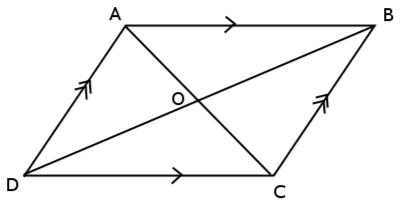
\includegraphics{
col11306.imgs/m39352_geomproof1.png} % ;geomproof1.png;;;6.0;8.5;
\vspace{2pt}
\vspace{.1in}
\end{center}
\end{figure}   
\westep{}    
Given: $AB\parallel CD$ and $AD\parallel BC$. We need to prove $A=C$ and $B=D$.
In the formal language of maths we say that we are required to prove (RTP)
$B\hat{A}D=B\hat{C}A$ and $A\hat{B}C=A\hat{D}C$. 

\westep{}
\begin{equation*}
\begin{array}{cccc}\hfill B\hat{A}C& =& A\hat{C}D\hfill &
(\mathrm{corresponding\; angles})\\ \hfill D\hat{A}C& =& B\hat{C}A\hfill &
(\mathrm{corresponding\; angles})\\ \hfill B\hat{A}D& =& B\hat{C}A\hfill &
\end{array}
\end{equation*}
Similarly we find that: 
\begin{equation*}
A\hat{B}C=A\hat{D}C}
\end{equation*}
}
\end{wex}

 
\begin{wex}{Proofs - 2}{
In parallelogram ABCD, the bisectors of the angles (AW, BX, CY and DZ) have been
constructed:
\scalebox{1} % Change this value to rescale the drawing.
{
\begin{pspicture}(0,-1.52)(4.91375,1.52)
\pspolygon[linewidth=0.04](1.37375,0.94)(4.45375,0.96)(3.41375,-1.06)(0.37375,-1.06)
\psline[linewidth=0.04cm](1.35375,0.96)(2.49375,-1.5)
\psline[linewidth=0.04cm](3.41375,-1.06)(2.27375,1.5)
\psline[linewidth=0.04cm](0.35375,-1.06)(4.89375,0.46)
\psline[linewidth=0.04cm](4.45375,0.94)(0.21375,-0.38)
\psdots[dotsize=0.12](1.35375,0.7)
\psdots[dotsize=0.12](1.51375,0.84)
\psdots[dotsize=0.12](3.23375,-0.92)
\psdots[dotsize=0.12](3.43375,-0.8)
\psdots[dotsize=0.08,dotstyle=triangle*](3.91375,0.86)
\psline[linewidth=0.02cm,arrowsize=0.233cm 3.0,arrowlength=0.67,arrowinset=0.67]{->}(2.45375,-1.06)(2.83375,-1.06)
\psline[linewidth=0.02cm,arrowsize=0.233cm 3.0,arrowlength=0.67,arrowinset=0.67]{->}(1.99375,0.94)(2.37375,0.94)
\psline[linewidth=0.02cm,arrowsize=0.233cm 3.0,arrowlength=0.67,arrowinset=0.67]{->>}(3.91375,-0.12)(3.97375,0.02)
\psline[linewidth=0.02cm,arrowsize=0.233cm 3.0,arrowlength=0.67,arrowinset=0.67]{->>}(0.93375,0.02)(1.09375,0.34)
\usefont{T1}{ptm}{m}{n}
\rput(1.3223437,0.485){\tiny 1}
\usefont{T1}{ptm}{m}{n}
\rput(1.681875,0.685){\tiny 2}
\usefont{T1}{ptm}{m}{n}
\rput(3.6623437,0.805){\tiny 1}
\usefont{T1}{ptm}{m}{n}
\rput(3.3623438,-0.615){\tiny 1}
\usefont{T1}{ptm}{m}{n}
\rput(1.0223438,-0.955){\tiny 1}
\usefont{T1}{ptm}{m}{n}
\rput(1.5423437,0.165){\tiny 1}
\usefont{T1}{ptm}{m}{n}
\rput(3.1823437,-0.275){\tiny 1}
\usefont{T1}{ptm}{m}{n}
\rput(2.8023438,0.585){\tiny 1}
\usefont{T1}{ptm}{m}{n}
\rput(1.9623437,-0.695){\tiny 1}
\usefont{T1}{ptm}{m}{n}
\rput(4.041875,0.625){\tiny 2}
\usefont{T1}{ptm}{m}{n}
\rput(3.061875,-0.875){\tiny 2}
\usefont{T1}{ptm}{m}{n}
\rput(0.701875,-0.795){\tiny 2}
\usefont{T1}{ptm}{m}{n}
\rput(1.921875,-0.015){\tiny 2}
\usefont{T1}{ptm}{m}{n}
\rput(2.861875,-0.115){\tiny 2}
\usefont{T1}{ptm}{m}{n}
\rput(2.101875,-0.355){\tiny 2}
\psdots[dotsize=0.08,dotstyle=triangle*](4.19375,0.76)
\psdots[dotsize=0.08,dotstyle=triangle*](0.55375,-0.92)
\psdots[dotsize=0.08,dotstyle=triangle*](0.79375,-1.0)
\usefont{T1}{ptm}{m}{n}
\rput(2.701875,0.245){\tiny 2}
\usefont{T1}{ptm}{m}{n}
\rput(1.2603126,1.11){A}
\usefont{T1}{ptm}{m}{n}
\rput(4.6009374,1.07){B}
\usefont{T1}{ptm}{m}{n}
\rput(3.4809375,-1.29){C}
\usefont{T1}{ptm}{m}{n}
\rput(0.11375,-1.19){D}
\usefont{T1}{ptm}{m}{n}
\rput(1.8329687,0.305){\scriptsize M}
\usefont{T1}{ptm}{m}{n}
\rput(3.0146875,0.325){\scriptsize N}
\usefont{T1}{ptm}{m}{n}
\rput(2.9445312,-0.375){\scriptsize O}
\usefont{T1}{ptm}{m}{n}
\rput(1.784375,-0.395){\scriptsize P}
\usefont{T1}{ptm}{m}{n}
\rput(0.6403125,-0.07){X}
\usefont{T1}{ptm}{m}{n}
\rput(2.639375,1.11){Y}
\usefont{T1}{ptm}{m}{n}
\rput(4.2364063,-0.03){Z}
\usefont{T1}{ptm}{m}{n}
\rput(2.0798438,-1.25){W}
\end{pspicture} 
}\\       
You are also given that $\mathrm{AB}=\mathrm{CD}$, $\mathrm{AD}=\mathrm{BC}$,
$\mathrm{AB}\parallel \mathrm{CD}$, $\mathrm{AD}\parallel \mathrm{BC}$, 
$\hat{A}=\hat{C}$, and $\hat{B}=\hat{D}$. 
Prove that MNOP is a parallelogram.} 
{

\westep{} 
Given: $\mathrm{AB}=\mathrm{CD}$, $\mathrm{AD}=\mathrm{BC}$,
$\mathrm{AB}\parallel \mathrm{CD}$, $\mathrm{AD}\parallel \mathrm{BC}$, 
$\hat{A}=\hat{C}$, and $\hat{B}=\hat{D}$. RTP: MNOP is a parallelogram.

\westep{} 
\begin{equation*}
\begin{array}{cc}\hfill
In\phantom{\rule{2pt}{0ex}}▵\phantom{\rule{2pt}{0ex}}\mathrm{ADW}\phantom{\rule{
2pt}{0ex}}\mathrm{and}\phantom{\rule{2pt}{0ex}}▵\mathrm{CBY}\phantom{\rule{2pt}{
0ex}}\\ \hfill D\hat{A}W& =&
B\hat{C}Y\phantom{\rule{2pt}{0ex}}(\mathrm{given})\hfill \\ \hfill A\hat{D}C& =&
A\hat{B}C\phantom{\rule{2pt}{0ex}}(\mathrm{given})\hfill \\ \hfill \mathrm{AD}&
=& \mathrm{BC}\phantom{\rule{2pt}{0ex}}\mathrm{(given)}\hfill \\ \hfill
\therefore \phantom{\rule{2pt}{0ex}}▵\mathrm{ADW}& =&
▵\mathrm{CBY}\phantom{\rule{2pt}{0ex}}\mathrm{(AAS)}\hfill \\ \hfill \therefore
\phantom{\rule{2pt}{0ex}}\mathrm{DW}& =& \mathrm{BY}\hfill
\end{array}\end{equation*}

\begin{equation*}
\begin{array}{cc}\hfill
In\phantom{\rule{2pt}{0ex}}▵\phantom{\rule{2pt}{0ex}}\mathrm{ABX}\phantom{\rule{
2pt}{0ex}}\mathrm{and}\phantom{\rule{2pt}{0ex}}▵\mathrm{CDZ}\phantom{\rule{2pt}{
0ex}}\\ \hfill D\hat{C}Z& =&
B\hat{A}X\phantom{\rule{2pt}{0ex}}(\mathrm{given})\hfill \\ \hfill Z\hat{D}C& =&
X\hat{B}A\phantom{\rule{2pt}{0ex}}(\mathrm{given})\hfill \\ \hfill \mathrm{DC}&
=& \mathrm{AB}\phantom{\rule{2pt}{0ex}}\mathrm{(given)}\hfill \\ \hfill
\therefore \phantom{\rule{2pt}{0ex}}▵\mathrm{ABX}& \equiv &
▵\mathrm{CDZ}\phantom{\rule{2pt}{0ex}}\mathrm{(AAS)}\hfill \\ \hfill \therefore
\phantom{\rule{2pt}{0ex}}\mathrm{AX}& =& \mathrm{CZ}\hfill \end{array}
\end{equation*}

\begin{equation*}
\begin{array}{cc}\hfill
In\phantom{\rule{2pt}{0ex}}▵\phantom{\rule{2pt}{0ex}}\mathrm{XAM}\phantom{\rule{
2pt}{0ex}}\mathrm{and}\phantom{\rule{2pt}{0ex}}▵\mathrm{ZCO}\phantom{\rule{2pt}{
0ex}}\\ \hfill X\hat{A}M& =&
Z\hat{C}O\phantom{\rule{2pt}{0ex}}(\mathrm{given})\hfill \\ \hfill A\hat{X}M& =&
C\hat{Z}O\phantom{\rule{2pt}{0ex}}(\mathrm{proven\; above})\hfill \\ \hfill
\mathrm{AX}& =& \mathrm{CZ}\phantom{\rule{2pt}{0ex}}\mathrm{(proven\;
above)}\hfill \\ \hfill \therefore \phantom{\rule{2pt}{0ex}}▵\mathrm{XAM}&
\equiv & ▵\mathrm{COZ}\phantom{\rule{2pt}{0ex}}\mathrm{(AAS)}\hfill \\ \hfill
\therefore \phantom{\rule{2pt}{0ex}}A\hat{O}C& =& A\hat{M}X\hfill \end{array}
\end{equation*}

\begin{equation*}
\begin{array}{ccc}\hfill A\hat{M}X& =&
P\hat{M}N\phantom{\rule{2pt}{0ex}}\mathrm{(vert.\; opp.\; \angle
\text{'}s)}\hfill \\ \hfill C\hat{O}Z& =&
N\hat{O}P\phantom{\rule{2pt}{0ex}}\mathrm{(vert.\; opp.\; \angle
\text{'}s)}\hfill \\ \hfill \therefore \phantom{\rule{2pt}{0ex}}P\hat{M}N& =&
N\hat{O}P\hfill \end{array}
\end{equation*}

\begin{equation*}
\begin{array}{cc}\hfill
In\phantom{\rule{2pt}{0ex}}▵\phantom{\rule{2pt}{0ex}}\mathrm{BYN}\phantom{\rule{
2pt}{0ex}}\mathrm{and}\phantom{\rule{2pt}{0ex}}▵\mathrm{DWP}\phantom{\rule{2pt}{
0ex}}\\ \hfill Y\hat{B}N& =&
W\hat{D}P\phantom{\rule{2pt}{0ex}}(\mathrm{given})\hfill \\ \hfill B\hat{Y}N& =&
W\hat{D}P\phantom{\rule{2pt}{0ex}}(\mathrm{proven\; above})\hfill \\ \hfill
\mathrm{DW}& =& \mathrm{BY}\phantom{\rule{2pt}{0ex}}\mathrm{(proven\;
above)}\hfill \\ \hfill \therefore \phantom{\rule{2pt}{0ex}}▵\mathrm{YBN}&
\equiv & ▵\mathrm{WDP}\phantom{\rule{2pt}{0ex}}\mathrm{(AAS)}\hfill \\ \hfill
\therefore \phantom{\rule{2pt}{0ex}}B\hat{N}Y& =& D\hat{P}W\hfill \end{array}
\end{equation*}

\begin{equation*}
\begin{array}{ccc}\hfill D\hat{P}W& =&
M\hat{P}O\phantom{\rule{2pt}{0ex}}\mathrm{(vert.\; opp.\; \angle
\text{'}s)}\hfill \\ \hfill B\hat{N}Y& =&
O\hat{N}M\phantom{\rule{2pt}{0ex}}\mathrm{(vert.\; opp.\; \angle
\text{'}s)}\hfill \\ \hfill \therefore \phantom{\rule{2pt}{0ex}}M\hat{P}O& =&
O\hat{N}M\hfill \end{array}
\end{equation*}
$\therefore $ MNOP is a parallelogram (both pairs opp. $\angle $'s $=$, and
therefore both pairs opp. sides parallel too)

\end{wex}



\Note{It is very important to note that a single counter example disproves a
conjecture. Also numerous specific supporting examples do not prove a
conjecture. }


\subsection{ Summary}
\begin{itemize}[noitemsep]
\item The properties of kites, rhombuses, parallelograms, squares, rectangles
and trapeziums was covered. These figures are all known as quadrilaterals\item
You should know the formulae for surface area of rectangular and triangular
prisms as well as cylinders\item 
The volume of a right prism is calculated by multiplying the area of the base by
the height. So, for a square prism of side length $a$ and height $h$ the volume
is $a\ensuremath{\times}a\ensuremath{\times}h={a}^{2}h$.\item 
Two polygons are similar if:\begin{itemize}[noitemsep]
\item their corresponding angles are equal\item the ratios of corresponding
sides are equal\end{itemize}
. All squares are similar\end{itemize}

\subsection{ End of Chapter Exercises}
\nopagebreak
\begin{enumerate}[noitemsep, label=\textbf{\arabic*}. ] 
\item Assess whether the following statements are true or false. If the
statement is false, explain why:
\begin{enumerate}[noitemsep, label=\textbf{\alph*}. ] 
\item  A trapezium is a quadrilateral with two pairs of parallel opposite
sides.\item  Both diagonals of a parallelogram bisect each other.\item  A
rectangle is a parallelogram that has all four corner angles equal to
60\ensuremath{{\,}^{\circ}}.\item  The four sides of a rhombus have different
lengths.\item  The diagonals of a kite intersect at right angles.\item  Two
polygons are similar if only their corresponding angles are
equal.\end{enumerate}
\item Calculate the area of each of the following shapes:
\setcounter{subfigure}{0}
\begin{figure}[H] % horizontal\label{m39358*id320600}
\begin{center}
\label{m39358*id320600!!!underscore!!!media}\label{
m39358*id320600!!!underscore!!!printimage}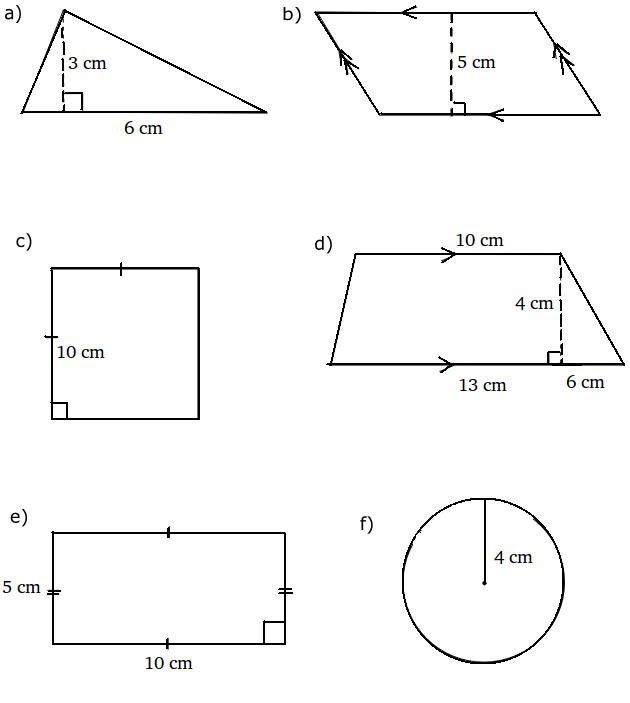
\includegraphics[height=300px]{
col11306.imgs/m39358_MG10C14_041.png} % m39358;MG10C14\_041.png;;;6.0;8.5;
\vspace{2pt}
\vspace{.1in}
\end{center}
\end{figure}              \item Calculate the surface area and volume of each of
the following objects (assume that all faces/surfaces are solid -- e.g. surface
area of cylinder will include circular areas at top and bottom):
\setcounter{subfigure}{0}
\begin{figure}[H] % horizontal\label{m39358*id320601}
\begin{center}
\label{m39358*id320601!!!underscore!!!media}\label{
m39358*id320601!!!underscore!!!printimage}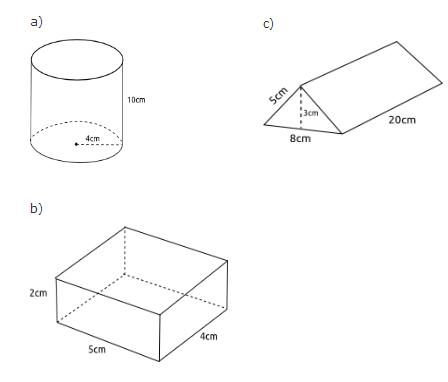
\includegraphics[width=300px]{
col11306.imgs/m39358_MG10C14_042.png} % m39358;MG10C14\_042.png;;;6.0;8.5;
\vspace{2pt}
\vspace{.1in}
\end{center}
\end{figure}              \item Calculate the surface area and volume of each of
the following objects (assume that all faces/surfaces are solid):
\setcounter{subfigure}{0}
\begin{figure}[H] % horizontal\label{m39358*id320602}
\begin{center}
\label{m39358*id320602!!!underscore!!!media}\label{
m39358*id320602!!!underscore!!!printimage}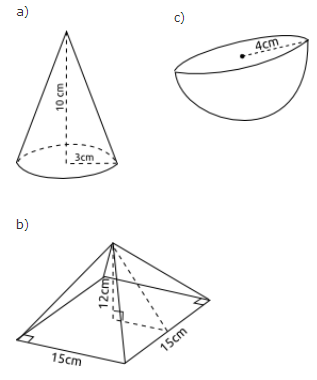
\includegraphics[height=300px]{
col11306.imgs/m39358_MG10C14_043.png} % m39358;MG10C14\_043.png;;;6.0;8.5;
\vspace{2pt}
\vspace{.1in}
\end{center}
\end{figure}               \item Using the rules given, identify the type of
transformation and draw the image of the shapes.
\label{m39358*id73963}\begin{enumerate}[noitemsep, label=\textbf{\alph*}. ] 
\label{m39358*uid126}\item  (x;y)$\to $(x+3;y-3)
\setcounter{subfigure}{0}
\begin{figure}[H] % horizontal\label{m39358*id73991}
\begin{center}
\label{m39358*id73991!!!underscore!!!media}\label{
m39358*id73991!!!underscore!!!printimage}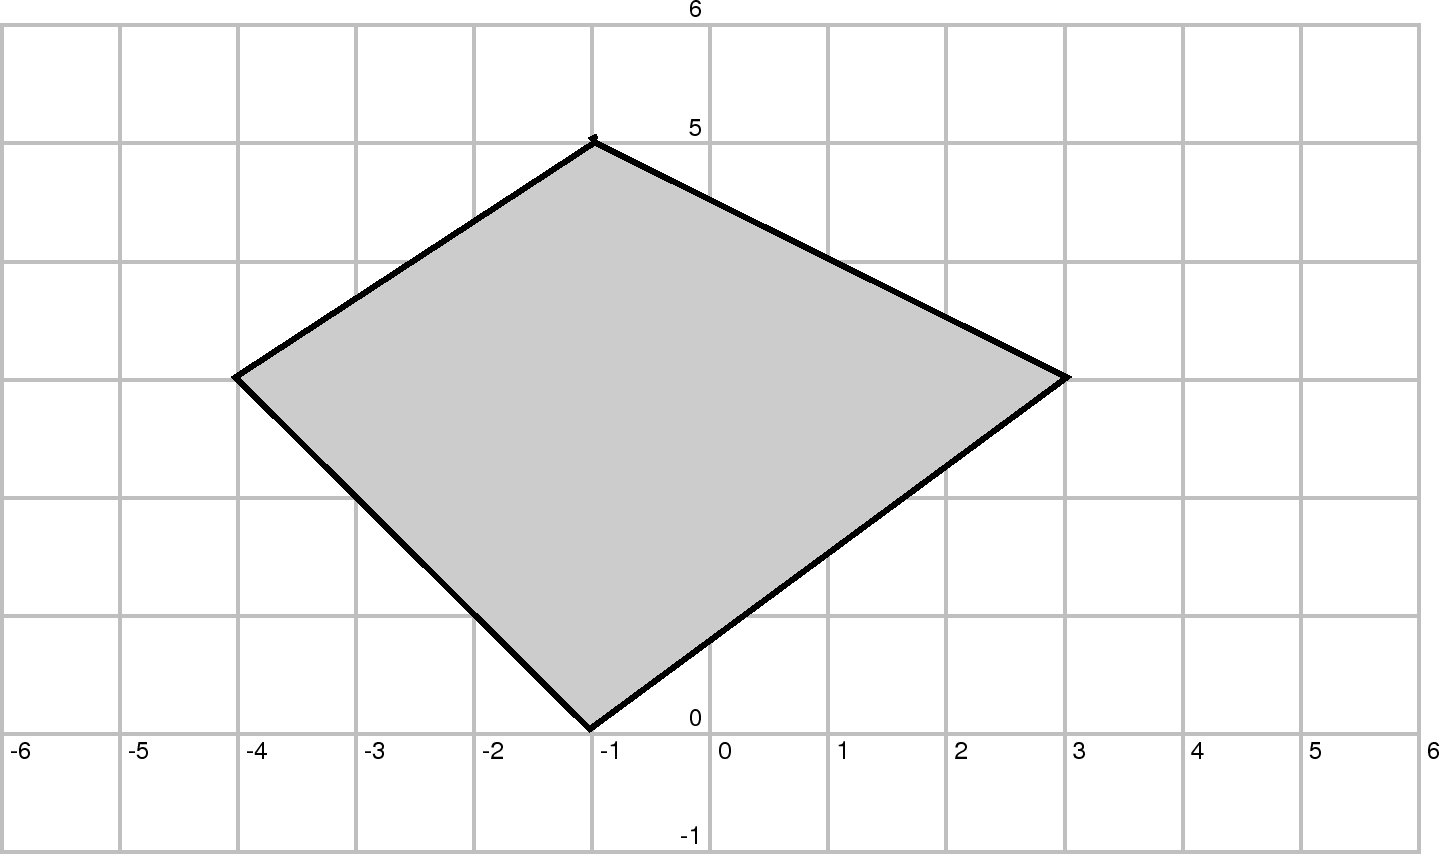
\includegraphics[width=300px]{
col11306.imgs/m39358_MG10C14_037.png} % m39358;MG10C14\_037.png;;;6.0;8.5;
\vspace{2pt}
\vspace{.1in}
\end{center}
\end{figure}     \item  (x;y)$\to $(x-4;y)
\setcounter{subfigure}{0}
\begin{figure}[H] % horizontal\label{m39358*id74022}
\begin{center}
\label{m39358*id74022!!!underscore!!!media}\label{
m39358*id74022!!!underscore!!!printimage}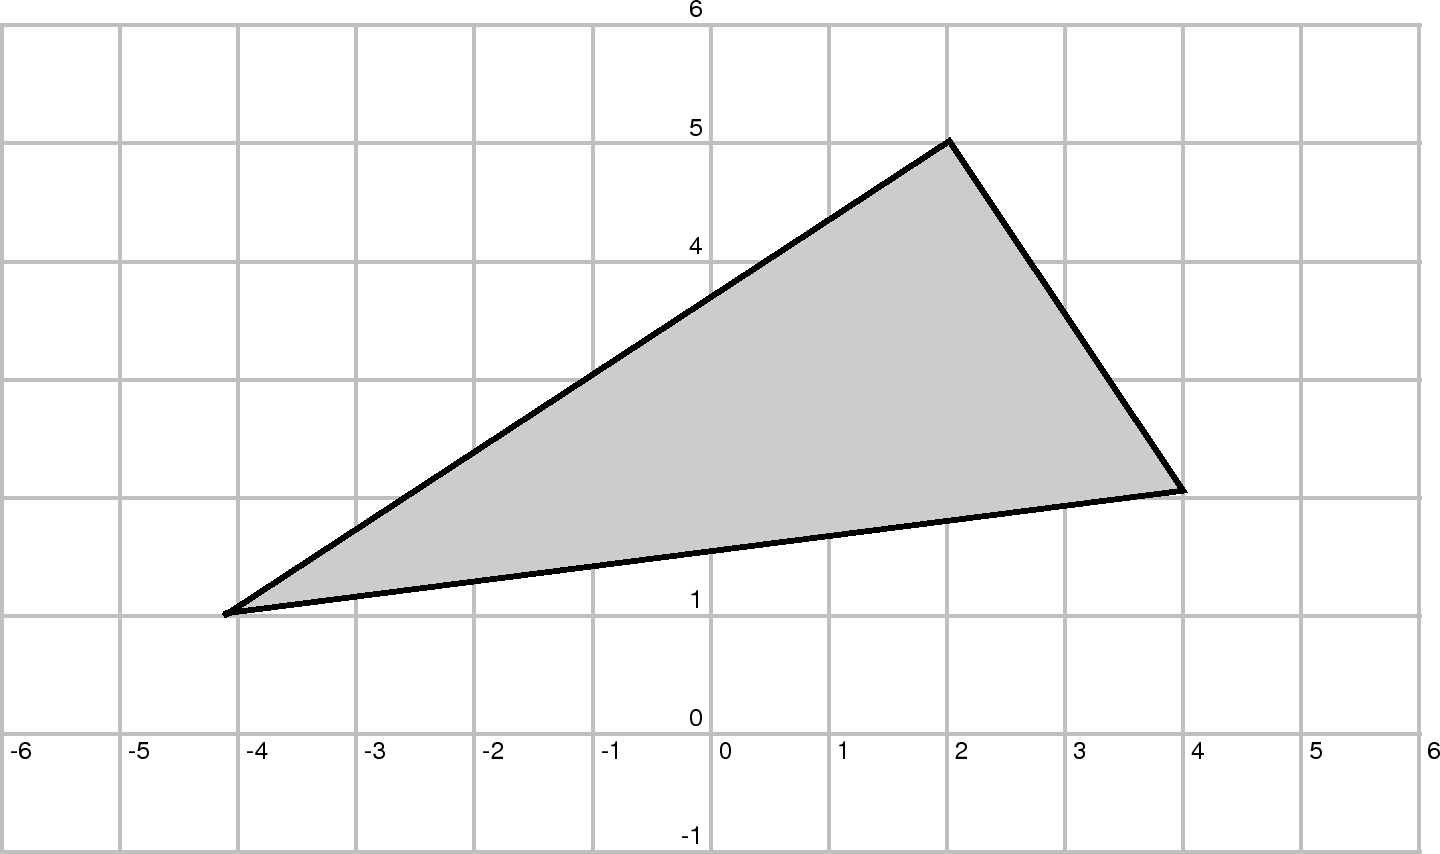
\includegraphics[width=300px]{
col11306.imgs/m39358_MG10C14_038.png} % m39358;MG10C14\_038.png;;;6.0;8.5;
\vspace{2pt}
\vspace{.1in}
\end{center}
\end{figure}       \item (x;y)$\to $(y;x)
\setcounter{subfigure}{0}
\begin{figure}[H] % horizontal\label{m39358*id74053}
\begin{center}
\label{m39358*id74053!!!underscore!!!media}\label{
m39358*id74053!!!underscore!!!printimage}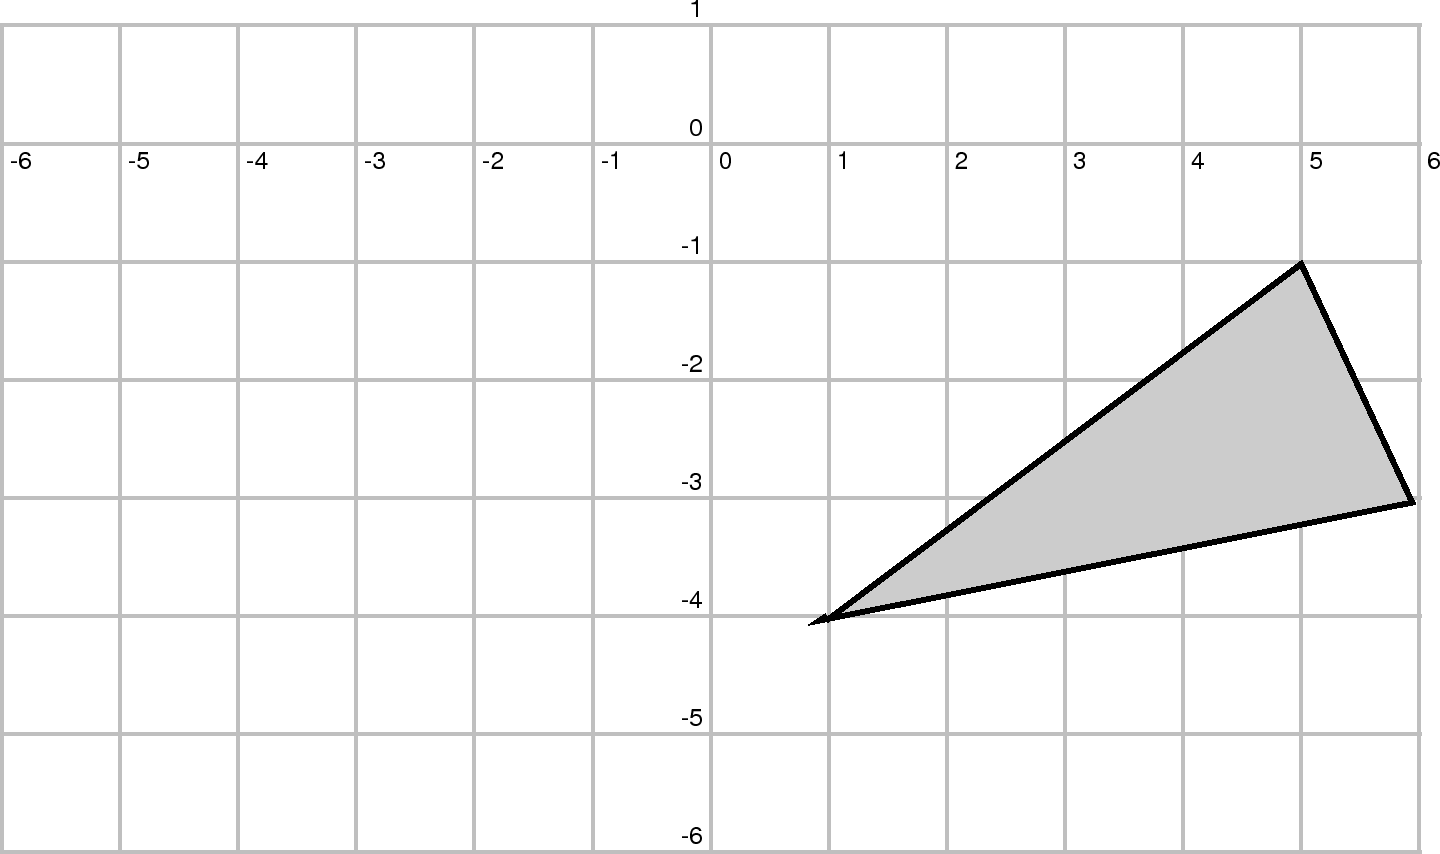
\includegraphics[width=300px]{
col11306.imgs/m39358_MG10C14_039.png} % m39358;MG10C14\_039.png;;;6.0;8.5;
\vspace{2pt}
\vspace{.1in}
\end{center}
\end{figure}      \item (x;y)$\to $(-x;-y)
\setcounter{subfigure}{0}
\begin{figure}[H] % horizontal\label{m39358*id74084}
\begin{center}
\label{m39358*id74084!!!underscore!!!media}\label{
m39358*id74084!!!underscore!!!printimage}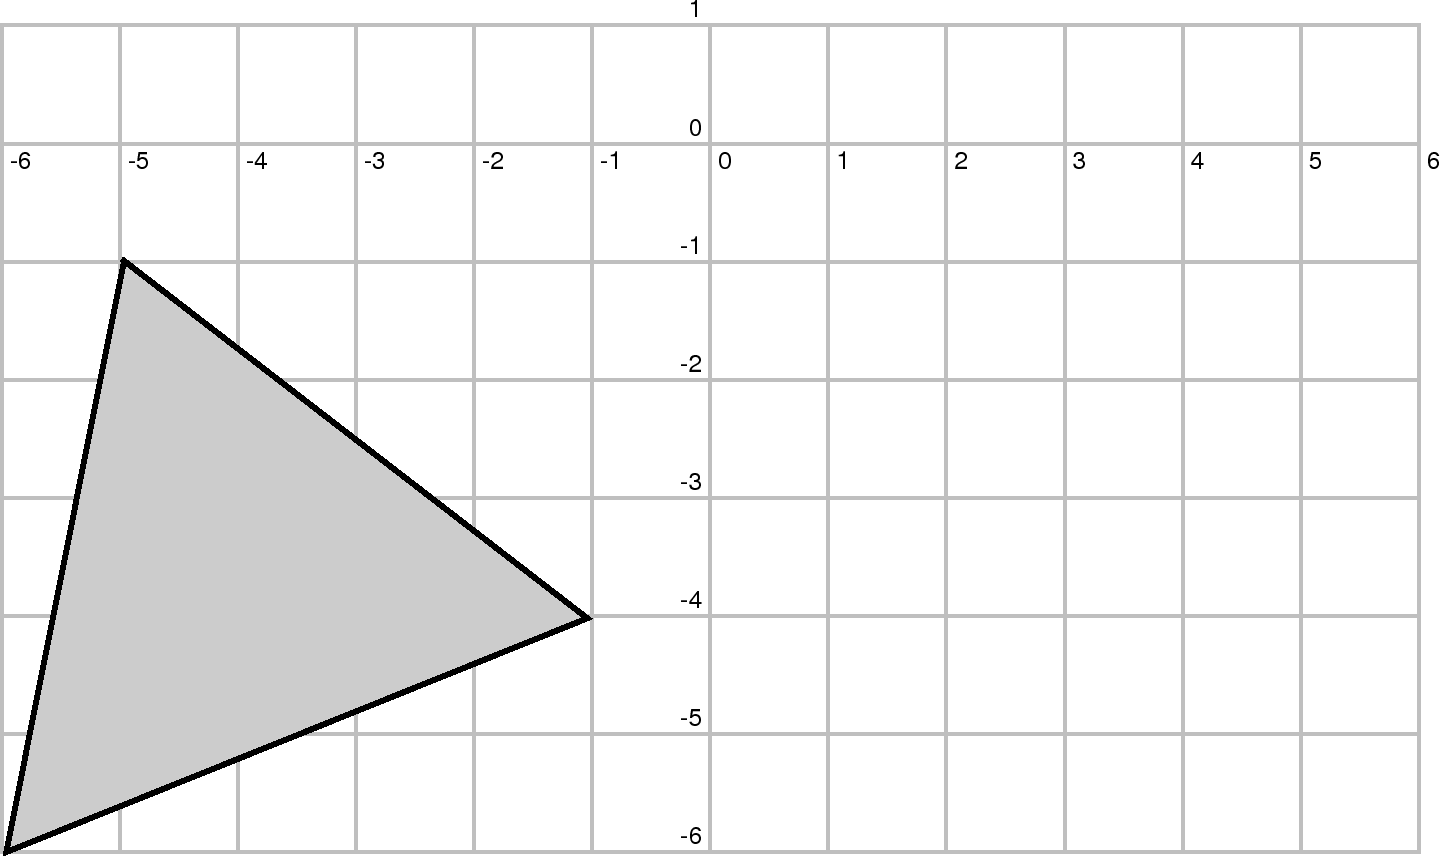
\includegraphics[width=300px]{
col11306.imgs/m39358_MG10C14_040.png} % m39358;MG10C14\_040.png;;;6.0;8.5;
\vspace{2pt}
\vspace{.1in}
\end{center}
\end{figure}       \end{enumerate}
  \item  
PQRS is a quadrilateral with points P(0; −3) ; Q(−2;5) ; R(3;2) and S(3;--2)  in
the Cartesian plane.
\begin{enumerate}[noitemsep, label=\textbf{\alph*}. ] 
\item Find the length of QR.\item Find the gradient of PS.\item Find the
midpoint of PR.\item Is PQRS a parallelogram?  Give reasons for your answer.
\end{enumerate}
  \item A(--2;3) and B(2;6) are points in the Cartesian plane.  C(a;b) is the
midpoint of AB. Find the values of a and b.\newline
\item 
Consider: Triangle ABC with vertices A (1; 3) B (4; 1) and C (6; 4):
\begin{enumerate}[noitemsep, label=\textbf{\alph*}. ] 
\item Sketch triangle ABC on the Cartesian plane. \item Show that ABC is an
isoceles triangle.\item Determine the co-ordinates of M, the midpoint of
AC.\item Determine the gradient of AB.\item Show that the following points are
collinear: A, B and D(7;-1)\end{enumerate}
\item In the diagram, A is the point (-6;1) and B is the point (0;3)
\setcounter{subfigure}{0}
\begin{figure}[H] % horizontal\label{m39358*id740344}
\begin{center}
\label{m39358*id740344!!!underscore!!!media}\label{
m39358*id740344!!!underscore!!!printimage}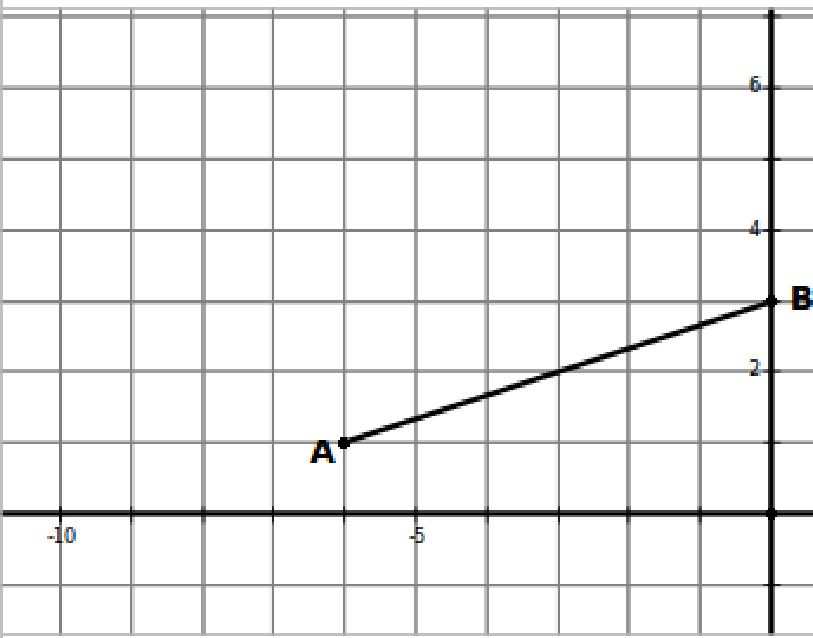
\includegraphics[width=.7\columnwidth]
{col11306.imgs/m39358_MG10C14_5.png} % m39358;MG10C14\_5.png;;;6.0;8.5;
\vspace{2pt}
\vspace{.1in}
\end{center}
\end{figure}       \begin{enumerate}[noitemsep, label=\textbf{\alph*}. ] 
\item Find the equation of line AB \item Calculate the length of AB\item  A' is
the image of A and B' is the image of B. Both these images are obtain by
applying the transformation: (x;y)$\to $(x-4;y-1). Give the coordinates of both
A' and B'\item Find the equation of A'B'\item Calculate the length of A'B'\item
Can you state with certainty that AA'B'B is a parallelogram? Justify your
answer.\end{enumerate}
    \item The vertices of triangle PQR have co-ordinates as shown in the
diagram.
\setcounter{subfigure}{0}
\begin{figure}[H] % horizontal\label{m39358*id743344}
\begin{center}
\label{m39358*id743344!!!underscore!!!media}\label{
m39358*id743344!!!underscore!!!printimage}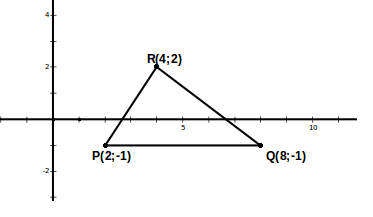
\includegraphics[width=300px]{
col11306.imgs/m39358_mg10c14_6.png} % m39358;mg10c14\_6.png;;;6.0;8.5;
\vspace{2pt}
\vspace{.1in}
\end{center}
\end{figure}       
\begin{enumerate}[noitemsep, label=\textbf{\alph*}. ] 
\item Give the co-ordinates of  P', Q' and R', the images of P, Q and R when P,
Q and R are reflected in the line y=x.\item Determine the area of triangle
PQR.\end{enumerate}
\item Which of the following claims are true? Give a counter-example for those
that are incorrect.
\begin{enumerate}[noitemsep, label=\textbf{\alph*}. ] 
\item All equilateral triangles are similar.
\item All regular quadrilaterals are similar.
\item In any $▵ABC$ with $\angle ABC={90}^{\circ }$ we have
$A{B}^{3}+B{C}^{3}=C{A}^{3}$.
\item All right-angled isosceles triangles with perimeter 10 cm are congruent.
\item All rectangles with the same area are similar.
\end{enumerate}
\item For each pair of figures state whether they are similar or not. Give
reasons.
\setcounter{subfigure}{0}
\begin{figure}[H] % horizontal\label{m39358*id320590}
\begin{center}
\label{m39358*id320590!!!underscore!!!media}\label{
m39358*id320590!!!underscore!!!printimage}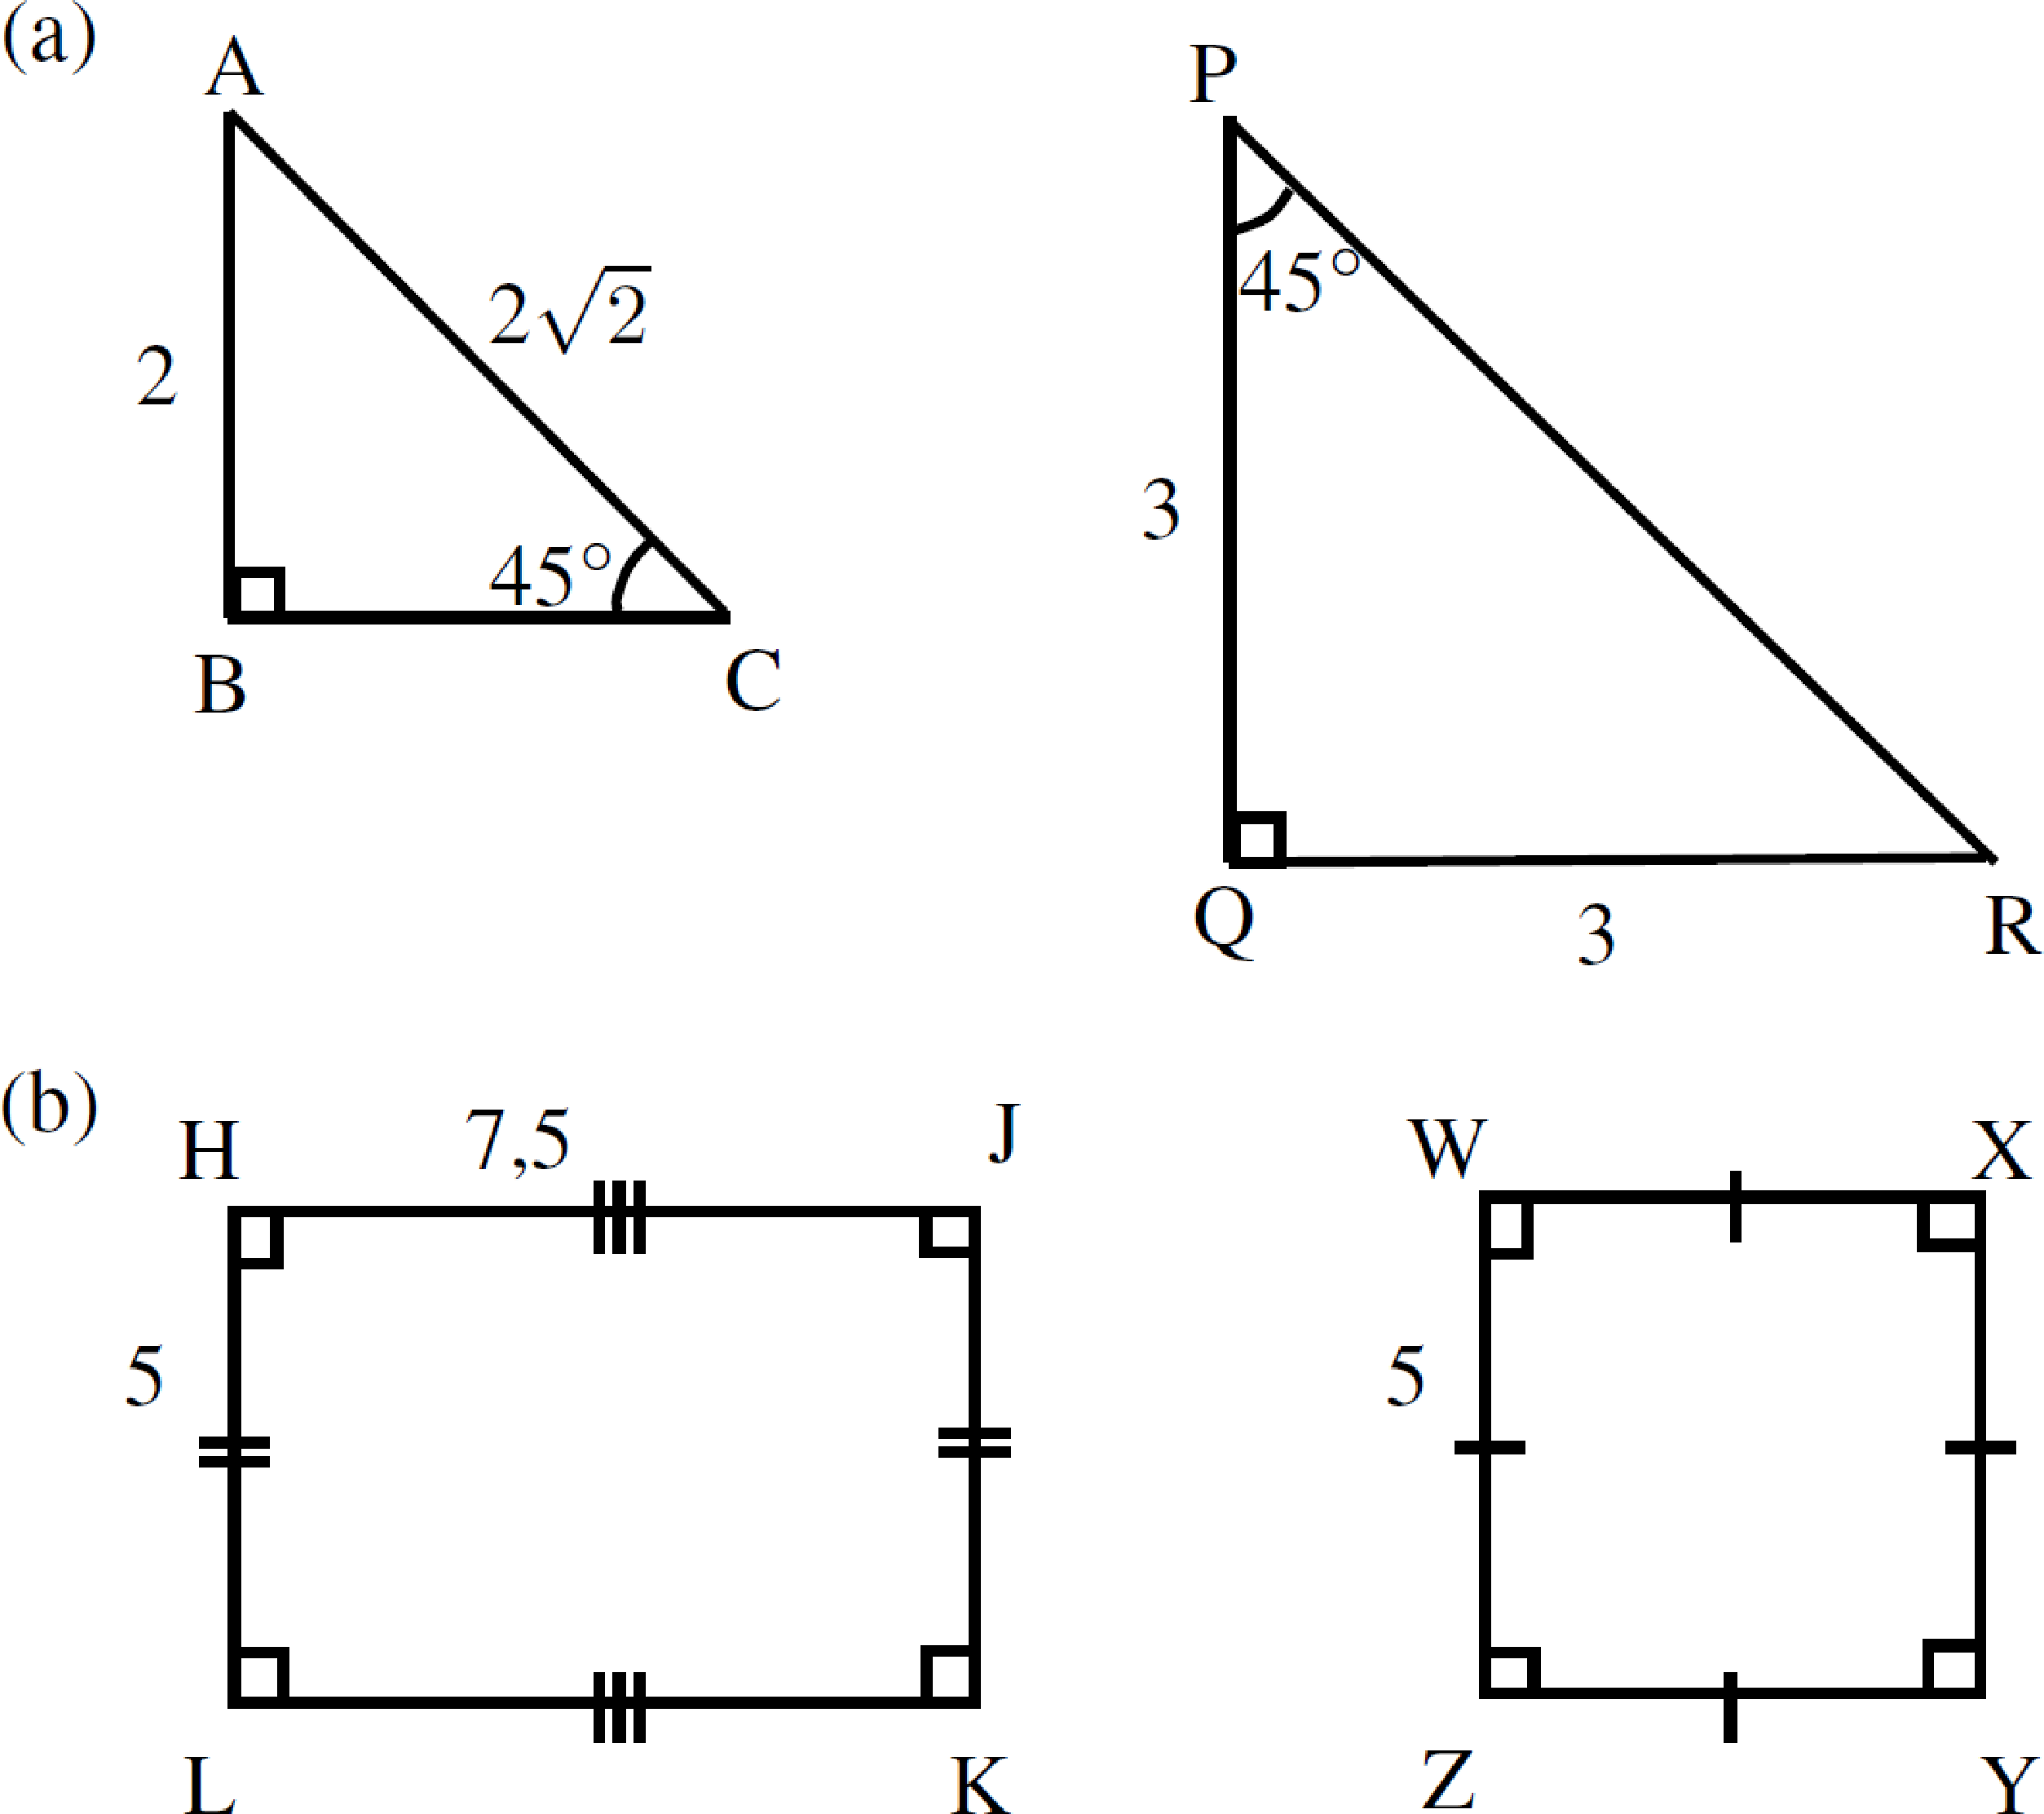
\includegraphics[width=.8\columnwidth]
{col11306.imgs/m39358_MG10C13_053.png} % m39358;MG10C13\_053.png;;;6.0;8.5;
\vspace{2pt}
\vspace{.1in}
\end{center}
\end{figure}               \end{enumerate}

\par \raisebox{-5
pt}{
\includegraphics[width=0.5cm]{col11306.imgs/summary_www.png}} Find the
answers with the shortcodes:
\par \begin{tabular}[h]{cccccc}
(1.) lbr  &  (2.) lT9  &  (3.) lTX  &  (4.) lTI  &  (5.) la7  &  (6.) laY  & 
(7.) laq  &  (8.) la4  &  (9.) l4o  &  (10.) laG  &  (11.) lal  &  (12.) la3  &
\end{tabular}

\subsection{ Summary}
\begin{itemize}[noitemsep]
\item Make sure you know what the following terms mean: quadrilaterals,
vertices, sides, angles, parallel lines, perpendicular lines,diagonals,
bisectors and transversals.\item The properties of triangles has been
covered.\item Congruency and similarity of triangles\item Angles can be
classified as acute, right, obtuse, straight, reflex or revolution\item Theorem
of Pythagoras which is used to calculate the lengths of sides of a right-angled
triangle\item Angles: 
\begin{itemize}[noitemsep]
\item Acute angle: An angle ${0}^{\circ }$ and ${90}^{\circ }$\item Right angle:
An angle measuring ${90}^{\circ }$\item Obtuse angle: An angle ${90}^{\circ }$
and ${180}^{\circ }$\item Straight angle: An angle measuring ${180}^{\circ
}$\item Reflex angle: An angle ${180}^{\circ }$ and ${360}^{\circ }$\item
Revolution: An angle measuring ${360}^{\circ }$\end{itemize}
\item There are several properties of angles and some special names for
these\item There are four types of triangles: Equilateral, isoceles,
right-angled and scalene\item The angles in a triangle add up to ${180}^{\circ
}$\end{itemize}

\subsection{ Exercises}
\nopagebreak
\begin{enumerate}[noitemsep, label=\textbf{\arabic*}. ] 
\item Find all the pairs of parallel lines in the following figures, giving
reasons in each case.
\begin{enumerate}[noitemsep, label=\textbf{\alph*}. ] 
\item 
\setcounter{subfigure}{0}
\begin{figure}[H] % horizontal\label{m39368*id320164}
\begin{center}
\label{m39368*id320164!!!underscore!!!media}\label{
m39368*id320164!!!underscore!!!printimage}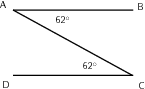
\includegraphics{
col11306.imgs/m39368_MG10C13_054.png} % m39368;MG10C13\_054.png;;;6.0;8.5;
\vspace{2pt}
\vspace{.1in}
\end{center}
\end{figure}       
\item 
\setcounter{subfigure}{0}
\begin{figure}[H] % horizontal\label{m39368*id320183}
\begin{center}
\label{m39368*id320183!!!underscore!!!media}\label{
m39368*id320183!!!underscore!!!printimage}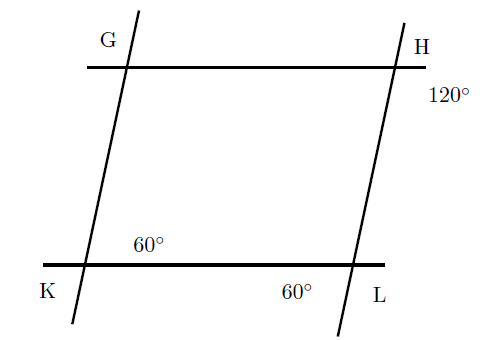
\includegraphics{
col11306.imgs/m39368_MG10C13_055.png} % m39368;MG10C13\_055.png;;;6.0;8.5;
\vspace{2pt}
\vspace{.1in}
\end{center}
\end{figure}       
\item 
\setcounter{subfigure}{0}
\begin{figure}[H] % horizontal\label{m39368*id320201}
\begin{center}
\label{m39368*id320201!!!underscore!!!media}\label{
m39368*id320201!!!underscore!!!printimage}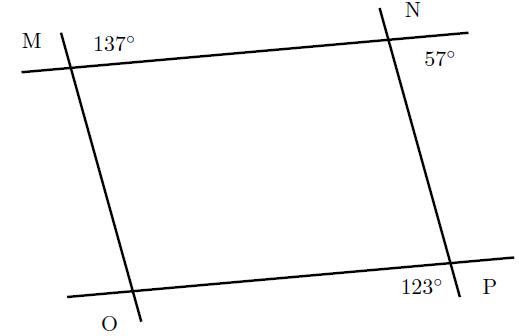
\includegraphics{
col11306.imgs/m39368_MG10C13_056.png} % m39368;MG10C13\_056.png;;;6.0;8.5;
\vspace{2pt}
\vspace{.1in}
\end{center}
\end{figure}       
\end{enumerate}
\item Find angles $a$, $b$, $c$ and $d$ in each case, giving reasons.
}\begin{enumerate}[noitemsep, label=\textbf{\alph*}. ] 
\item 
\setcounter{subfigure}{0}
\begin{figure}[H] % horizontal\label{m39368*id320271}
\begin{center}
\label{m39368*id320271!!!underscore!!!media}\label{
m39368*id320271!!!underscore!!!printimage}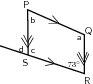
\includegraphics{
col11306.imgs/m39368_MG10C13_057.png} % m39368;MG10C13\_057.png;;;6.0;8.5;
\vspace{2pt}
\vspace{.1in}
\end{center}
\end{figure}         
\section{ Polygons and quadrilaterals}
\nopagebreak
 $ \hspace{-5pt}\begin{array}{cccccccccccc}  

\includegraphics[width=0.75cm]{col11306.imgs/summary_fullmarks.png} &  
\end{array} $ \hspace{2 pt}\raisebox{-5 pt}{} {(section shortcode: MG10093 )}
\par 
\item 
\setcounter{subfigure}{0}
\begin{figure}[H] % horizontal\label{m39368*id320290}
\begin{center}
\label{m39368*id320290!!!underscore!!!media}\label{
m39368*id320290!!!underscore!!!printimage}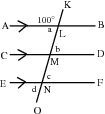
\includegraphics{
col11306.imgs/m39368_MG10C13_058.png} % m39368;MG10C13\_058.png;;;6.0;8.5;
\vspace{2pt}
\vspace{.1in}
\end{center}
\section{ Polygons and quadrilaterals}

 $ \hspace{-5pt}\begin{array}{cccccccccccc}  

\includegraphics[width=0.75cm]{col11306.imgs/summary_fullmarks.png} &  
\end{array} $ \hspace{2 pt}\raisebox{-5 pt}{} {(section shortcode: MG10093 )}
\par 
\end{figure}       

\item 
\setcounter{subfigure}{0}
\begin{figure}[H] % horizontal\label{m39368*id320310}
\begin{center}
\label{m39368*id320310!!!underscore!!!media}\label{
m39368*id320310!!!underscore!!!printimage}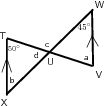
\includegraphics{
col11306.imgs/m39368_MG10C13_059.png} % m39368;MG10C13\_059.png;;;6.0;8.5;
\vspace{2pt}
\vspace{.1in}
\end{center}
\end{figure}       \end{enumerate}
\item Say which of the following pairs of triangles are congruent with reasons.
\begin{enumerate}[noitemsep, label=\textbf{\alph*}. ] 
\item 
\setcounter{subfigure}{0}
\begin{figure}[H] % horizontal\label{m39368*id320512}
\begin{center}
\label{m39368*id320512!!!underscore!!!media}\label{
m39368*id320512!!!underscore!!!printimage}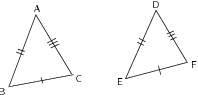
\includegraphics{
col11306.imgs/m39368_MG10C13_060.png} % m39368;MG10C13\_060.png;;;6.0;8.5;
\vspace{2pt}
\vspace{.1in}
\end{center}
\end{figure}       
\item 
\setcounter{subfigure}{0}
\begin{figure}[H] % horizontal\label{m39368*id320530}
\begin{center}
\label{m39368*id320530!!!underscore!!!media}\label{
m39368*id320530!!!underscore!!!printimage}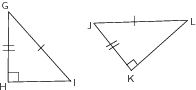
\includegraphics{
col11306.imgs/m39368_MG10C13_061.png} % m39368;MG10C13\_061.png;;;6.0;8.5;
\vspace{2pt}
\vspace{.1in}
\end{center}
\end{figure}     
\item 
\setcounter{subfigure}{0}
\begin{figure}[H] % horizontal\label{m39368*id320548}
\begin{center}
\label{m39368*id320548!!!underscore!!!media}\label{
m39368*id320548!!!underscore!!!printimage}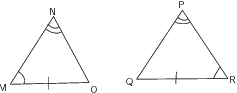
\includegraphics{
col11306.imgs/m39368_MG10C13_062.png} % m39368;MG10C13\_062.png;;;6.0;8.5;
\vspace{2pt}
\vspace{.1in}
\end{center}
\end{figure}       

\item 
\setcounter{subfigure}{0}
\begin{figure}[H] % horizontal\label{m39368*id320565}
\begin{center}
\label{m39368*id320565!!!underscore!!!media}\label{
m39368*id320565!!!underscore!!!printimage}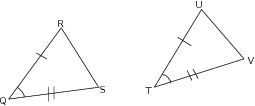
\includegraphics{
col11306.imgs/m39368_MG10C13_063.png} % m39368;MG10C13\_063.png;;;6.0;8.5;
\vspace{2pt}
\vspace{.1in}
\end{center}
\end{figure}       \end{enumerate}
\item Identify the types of angles shown below (e.g. acute/obtuse etc):
\setcounter{subfigure}{0}
\begin{figure}[H] % horizontal\label{m39368*id401231}
\begin{center}
\label{m39368*id401231!!!underscore!!!media}\label{
m39368*id401231!!!underscore!!!printimage}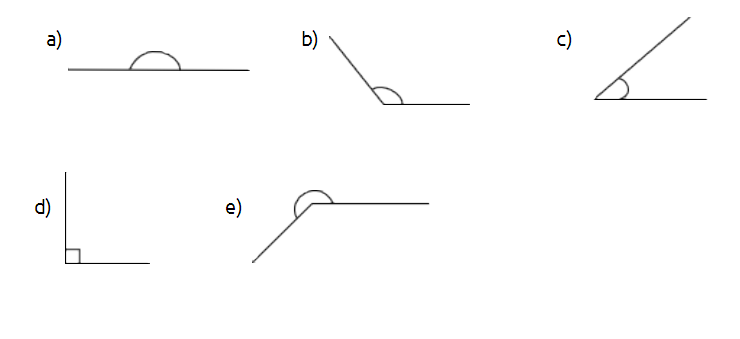
\includegraphics[width=300px]{
col11306.imgs/m39368_MG10C13_066.png} % m39368;MG10C13\_066.png;;;6.0;8.5;
\vspace{2pt}
\vspace{.1in}
\end{center}
\end{figure}       
\item Calculate the size of the third angle (x) in each of the diagrams below:
\setcounter{subfigure}{0}
\begin{figure}[H] % horizontal\label{m39368*id401232}
\begin{center}
\label{m39368*id401232!!!underscore!!!media}\label{
m39368*id401232!!!underscore!!!printimage}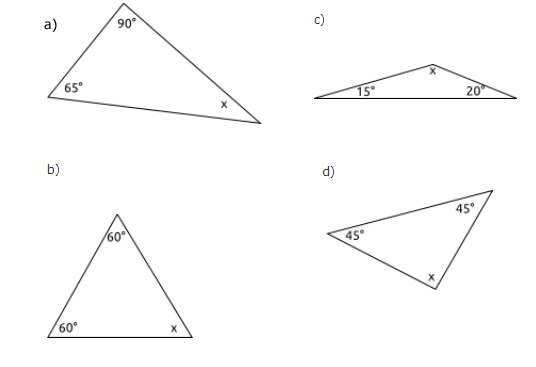
\includegraphics[width=300px]{
col11306.imgs/m39368_MG10C13_067.png} % m39368;MG10C13\_067.png;;;6.0;8.5;
\vspace{2pt}
\vspace{.1in}
\end{center}
\end{figure}       

\item Name each of the shapes/polygons, state how many sides each has and
whether it is regular (equiangular and equilateral) or not:
\setcounter{subfigure}{0}
\begin{figure}[H] % horizontal\label{m39368*id401233}
\begin{center}
\label{m39368*id401233!!!underscore!!!media}\label{
m39368*id401233!!!underscore!!!printimage}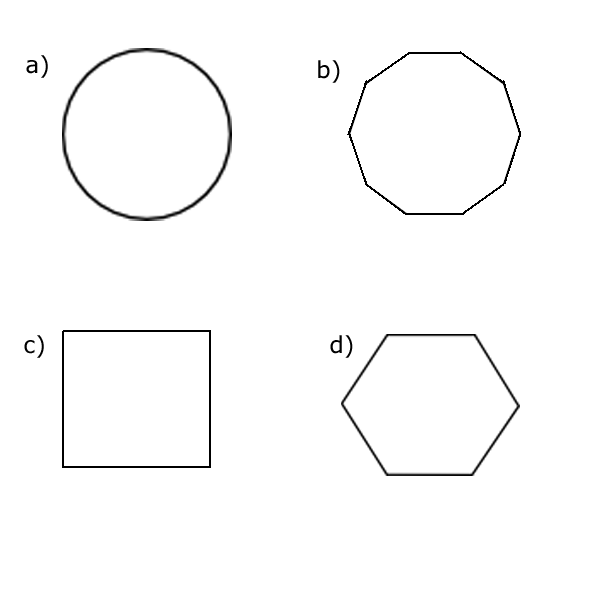
\includegraphics[width=300px]{
col11306.imgs/m39368_MG10C13_068.png} % m39368;MG10C13\_068.png;;;6.0;8.5;
\vspace{2pt}
\vspace{.1in}
\end{center}
\end{figure}       
\item Assess whether the following statements are true or false. If the
statement is false, explain why:
\begin{enumerate}[noitemsep, label=\textbf{\alph*}. ] 
\item An angle is formed when two straight lines meet at a point.	\item
The smallest angle that can be drawn is 5\ensuremath{{\,}^{\circ}}.\item An
angle of 90\ensuremath{{\,}^{\circ}} is called a square angle.\item Two angles
whose sum is 180\ensuremath{{\,}^{\circ}} are called supplementary angles.\item
Two parallel lines will never intersect.\item A regular polygon has equal angles
but not equal sides.\item An isoceles triangle has three equal sides.\item If
three sides of a triangle are equal in length to the same sides of another
triangle, then the two triangles are incongruent.\item If three pairs of
corresponding angles in two triangles are equal, then the triangles are
similar.\end{enumerate}
\item Name the type of angle (e.g. acute/obtuse etc) based on it's size:
\begin{enumerate}[noitemsep, label=\textbf{\alph*}. ] 
\item  30\ensuremath{{\,}^{\circ}}\item  47\ensuremath{{\,}^{\circ}}\item 
90\ensuremath{{\,}^{\circ}}\item  91\ensuremath{{\,}^{\circ}}\item 
191\ensuremath{{\,}^{\circ}}\item  360\ensuremath{{\,}^{\circ}}\item 
180\ensuremath{{\,}^{\circ}}\end{enumerate}
\item Using Pythagoras' theorem for right-angled triangles, calculate the length
of x:
\setcounter{subfigure}{0}
\begin{figure}[H] % horizontal\label{m39368*id401236}
\begin{center}
\label{m39368*id401236!!!underscore!!!media}\label{
m39368*id401236!!!underscore!!!printimage}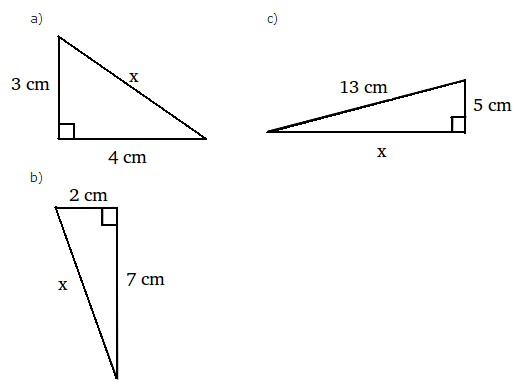
\includegraphics[width=300px]{
col11306.imgs/m39368_MG10C13_070.png} % m39368;MG10C13\_070.png;;;6.0;8.5;
\vspace{2pt}
\vspace{.1in}
\end{center}
\end{figure}       
\end{enumerate}

\par \raisebox{-5
pt}{
\includegraphics[width=0.5cm]{col11306.imgs/summary_www.png}} Find the
answers with the shortcodes:
\par \begin{tabular}[h]{cccccc}
(1.) lxh  &  (2.) laq  &  (3.) lai  &  (4.) lTb  &  (5.) lTj  &  (6.) lTD  & 
(7.) lTZ  &  (8.) lTB  &  (9.) lTK  & \end{tabular}
\subsubsection{ Challenge Problem}
\begin{enumerate}[noitemsep, label=\textbf{\arabic*}. ] 
\item Using the figure below, show that the sum of the three angles in a
triangle is 180$^{\circ }$. Line $DE$ is parallel to $BC$.
\setcounter{subfigure}{0}
\begin{figure}[H] % horizontal\label{m39368*id320668}
\begin{center}
\label{m39368*id320668!!!underscore!!!media}\label{
m39368*id320668!!!underscore!!!printimage}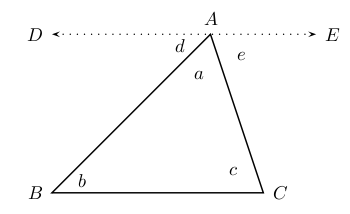
\includegraphics{
col11306.imgs/m39368_MG10C13_065.png} % m39368;MG10C13\_065.png;;;6.0;8.5;
\vspace{2pt}
\vspace{.1in}
\end{center}
\end{figure}       \newline
\end{enumerate}

\par \raisebox{-5
pt}{
\includegraphics[width=0.5cm]{col11306.imgs/summary_www.png}} Find the
answers with the shortcodes:
\par \begin{tabular}[h]{cccccc}
(1.) laO  & \end{tabular}

        \section{Exercises}
        \nopagebreak
        \label{m38380} $ \hspace{-5pt}\begin{array}{cccccccccccc}   \end{array}
$ \hspace{2 pt}\raisebox{-5
pt}{
\includegraphics[width=0.5cm]{col11306.imgs/summary_www.png}} {(section
shortcode: P10120 )} \par \label{m38380*id320135}\begin{enumerate}[noitemsep,
label=\textbf{\arabic*}. ] 
            \label{m38380*uid112}\item Find all the pairs of parallel lines in
the following figures, giving reasons in each case.

%\label{m38380*eip-78}\begin{enumerate}[noitemsep, label=\textbf{\alph*}. ] 
 %           \label{m38380*uid113}\item 
          
    \setcounter{subfigure}{0}


	\begin{figure}[H] % horizontal\label{m38380*id320164}
    \begin{center}
   
\label{m38380*id320164!!!underscore!!!media}\label{
m38380*id320164!!!underscore!!!printimage}\includegraphics[width=0.7\textwidth]{
col11306.imgs/m38380_MG10C13_054.png} % m38380;MG10C13\_054.png;;;6.0;8.5;
        
   %   \vspace{2pt}
   % \vspace{.1in}
    
    \end{center}

 \end{figure}   

    \addtocounter{footnote}{-0}
    
%        \label{m38380*uid114}\item 
          
 %   \setcounter{subfigure}{0}


%	\begin{figure}[H] % horizontal\label{m38380*id320183}
  %  \begin{center}
 %  
\label{m38380*id320183!!!underscore!!!media}\label{
m38380*id320183!!!underscore!!!printimage}\includegraphics[width=0.3\textwidth]{
col11306.imgs/m38380_MG10C13_055.png} % m38380;MG10C13\_055.png;;;6.0;8.5;
        
   %   \vspace{2pt}
   % \vspace{.1in}
    
   % \end{center}

 %\end{figure}   

  %  \addtocounter{footnote}{-0}
    
  %      \label{m38380*uid115}\item 
          
  %  \setcounter{subfigure}{0}


%	\begin{figure}[H] % horizontal\label{m38380*id320201}
%    \begin{center}
%   
\label{m38380*id320201!!!underscore!!!media}\label{
m38380*id320201!!!underscore!!!printimage}\includegraphics[width=0.3\textwidth]{
col11306.imgs/m38380_MG10C13_056.png} % m38380;MG10C13\_056.png;;;6.0;8.5;
        
  %    \vspace{2pt}
 %   \vspace{.1in}
    
  %  \end{center}

% \end{figure}   

 %   \addtocounter{footnote}{-0}
    
  %      \end{enumerate}
        
        \label{m38380*uid116}\item Find angles \begin{math}a\end{math},
\begin{math}b\end{math}, \begin{math}c\end{math} and \begin{math}d\end{math} in
each case, giving reasons.
%\label{m38380*id320255}\begin{enumerate}[noitemsep, label=\textbf{\alph*}. ] 
 %           \label{m38380*uid117}\item 
    \setcounter{subfigure}{0}


	\begin{figure}[H] % horizontal\label{m38380*id320271}
    \begin{center}
   
\label{m38380*id320271!!!underscore!!!media}\label{
m38380*id320271!!!underscore!!!printimage}\includegraphics[width=0.7\textwidth]{
col11306.imgs/m38380_MG10C13_057.png} % m38380;MG10C13\_057.png;;;6.0;8.5;
        
   %   \vspace{2pt}
   % \vspace{.1in}
    
    \end{center}

 \end{figure}   

    \addtocounter{footnote}{-0}
 %   \label{m38380*uid118}\item 
  %  \setcounter{subfigure}{0}


%	\begin{figure}[H] % horizontal\label{m38380*id320290}
%    \begin{center}
 %  
\label{m38380*id320290!!!underscore!!!media}\label{
m38380*id320290!!!underscore!!!printimage}\includegraphics[width=0.2\textwidth]{
col11306.imgs/m38380_MG10C13_058.png} % m38380;MG10C13\_058.png;;;6.0;8.5;
        
  %    \vspace{2pt}
  %  \vspace{.1in}
    
   % \end{center}

 %\end{figure}   

  %  \addtocounter{footnote}{-0}
  %  \label{m38380*uid119}\item 
  %  \setcounter{subfigure}{0}


%	\begin{figure}[H] % horizontal\label{m38380*id320310}
 %   \begin{center}
  % 
\label{m38380*id320310!!!underscore!!!media}\label{
m38380*id320310!!!underscore!!!printimage}\includegraphics[width=0.2\textwidth]{
col11306.imgs/m38380_MG10C13_059.png} % m38380;MG10C13\_059.png;;;6.0;8.5;
        
   %   \vspace{2pt}
  %  \vspace{.1in}
    
   % \end{center}

 %\end{figure}   

  %  \addtocounter{footnote}{-0}
  %  \end{enumerate}
        
        
\label{m38380*uid126}\item Say which of the following pairs of triangles are
congruent with reasons.
%\label{m38380*id320498}\begin{enumerate}[noitemsep, label=\textbf{\alph*}. ] 
 %           \label{m38380*uid127}\item 
    \setcounter{subfigure}{0}


	\begin{figure}[H] % horizontal\label{m38380*id320512}
    \begin{center}
   
\label{m38380*id320512!!!underscore!!!media}\label{
m38380*id320512!!!underscore!!!printimage}\includegraphics[width=0.85\textwidth]
{col11306.imgs/m38380_MG10C13_060.png} % m38380;MG10C13\_060.png;;;6.0;8.5;
        
      \vspace{2pt}
    \vspace{.1in}
    
    \end{center}

 \end{figure}   

    \addtocounter{footnote}{-0}
  %  \label{m38380*uid128}\item 
   % \setcounter{subfigure}{0}


	%\begin{figure}[H] % horizontal\label{m38380*id320530}
   % \begin{center}
   %
\label{m38380*id320530!!!underscore!!!media}\label{
m38380*id320530!!!underscore!!!printimage}\includegraphics[width=0.4\textwidth]{
col11306.imgs/m38380_MG10C13_061.png} % m38380;MG10C13\_061.png;;;6.0;8.5;
        
   %   \vspace{2pt}
   % \vspace{.1in}
    
   % \end{center}

 %\end{figure}   

  %  \addtocounter{footnote}{-0}
  %  \label{m38380*uid129}\item 
  %  \setcounter{subfigure}{0}


%	\begin{figure}[H] % horizontal\label{m38380*id320548}
%    \begin{center}
%   
\label{m38380*id320548!!!underscore!!!media}\label{
m38380*id320548!!!underscore!!!printimage}\includegraphics[width=0.4\textwidth]{
col11306.imgs/m38380_MG10C13_062.png} % m38380;MG10C13\_062.png;;;6.0;8.5;
        
%      \vspace{2pt}
%    \vspace{.1in}
    
 %   \end{center}

 %\end{figure}   

  %  \addtocounter{footnote}{-0}
  %  \label{m38380*uid130}\item 
  %  \setcounter{subfigure}{0}


%	\begin{figure}[H] % horizontal\label{m38380*id320565}
%    \begin{center}
 %  
\label{m38380*id320565!!!underscore!!!media}\label{
m38380*id320565!!!underscore!!!printimage}\includegraphics[width=0.4\textwidth]{
col11306.imgs/m38380_MG10C13_063.png} % m38380;MG10C13\_063.png;;;6.0;8.5;
        
 %    \vspace{2pt}
 %   \vspace{.1in}
    
  %  \end{center}

 %\end{figure}   

  %  \addtocounter{footnote}{-0}
  %  \end{enumerate}
        

        \label{m38380*uid131}\item Identify the types of angles shown below
(e.g. acute/obtuse etc):

          
    \setcounter{subfigure}{0}


	\begin{figure}[H] % horizontal\label{m38380*id401231}
    \begin{center}
   
\label{m38380*id401231!!!underscore!!!media}\label{
m38380*id401231!!!underscore!!!printimage}\includegraphics[width=0.6\textwidth]{
col11306.imgs/m38380_MG10C13_066.png} % m38380;MG10C13\_066.png;;;6.0;8.5;
        
  %    \vspace{2pt}
   
   % \vspace{.1in}
    
    \end{center}

 \end{figure}   

    \addtocounter{footnote}{-0}
    
        
\label{m38380*uid140}\item Calculate the size of the third angle (x) in each of
the diagrams below:

          
    \setcounter{subfigure}{0}


	\begin{figure}[H] % horizontal\label{m38380*id401232}
    \begin{center}
   
\label{m38380*id401232!!!underscore!!!media}\label{
m38380*id401232!!!underscore!!!printimage}\includegraphics[width=0.5\textwidth]{
col11306.imgs/m38380_MG10C13_067.png} % m38380;MG10C13\_067.png;;;6.0;8.5;
        
 %     \vspace{2pt}
  %  \vspace{.1in}
    
    \end{center}

 \end{figure}   

    \addtocounter{footnote}{-0}
 \pagebreak   
        
\label{m38380*uid141}\item Name each of the shapes/polygons, state how many
sides each has and whether it is regular (equiangular and equilateral) or not:

          
    \setcounter{subfigure}{0}


	\begin{figure}[H] % horizontal\label{m38380*id401233}
    \begin{center}
   
\label{m38380*id401233!!!underscore!!!media}\label{
m38380*id401233!!!underscore!!!printimage}\includegraphics[width=0.6\textwidth]{
col11306.imgs/m38380_MG10C13_068.png} % m38380;MG10C13\_068.png;;;6.0;8.5;
        
 %     \vspace{2pt}
  %  \vspace{.1in}
    
    \end{center}

 \end{figure}   

    \addtocounter{footnote}{-0}
    
        
\label{m38380*uid142}\item Assess whether the following statements are true or
false. If the statement is false, explain why:
\label{m38380*id401234}\begin{enumerate}[noitemsep, label=\textbf{\alph*}. ] 
            \item An angle is formed when two straight lines meet at a point.
\item The smallest angle that can be drawn is 5\ensuremath{{\,}^{\circ}}.\item
An angle of 90\ensuremath{{\,}^{\circ}} is called a square angle.\item Two
angles whose sum is 180\ensuremath{{\,}^{\circ}} are called supplementary
angles.\item Two parallel lines will never intersect.\item A regular polygon has
equal angles but not equal sides.\item An isoceles triangle has three equal
sides.\item If three sides of a triangle are equal in length to the same sides
of another triangle, then the two triangles are incongruent.\item If three pairs
of corresponding angles in two triangles are equal, then the triangles are
similar.\end{enumerate}
        
        
\label{m38380*uid143}\item Name the type of angle (e.g. acute/obtuse etc) based
on it's size:
\label{m38380*id401235}\begin{enumerate}[noitemsep, label=\textbf{\alph*}. ] 
            \item  30\ensuremath{{\,}^{\circ}}\item 
47\ensuremath{{\,}^{\circ}}\item  90\ensuremath{{\,}^{\circ}}\item 
91\ensuremath{{\,}^{\circ}}\item  191\ensuremath{{\,}^{\circ}}\item 
360\ensuremath{{\,}^{\circ}}\item  180\ensuremath{{\,}^{\circ}}\end{enumerate}
        
 \pagebreak       
\label{m38380*uid144}\item Using Pythagoras' theorem for right-angled triangles,
calculate the length of x:

          
    \setcounter{subfigure}{0}


	\begin{figure}[H] % horizontal\label{m38380*id401236}
    \begin{center}
   
\label{m38380*id401236!!!underscore!!!media}\label{
m38380*id401236!!!underscore!!!printimage}\includegraphics[width=0.8\textwidth]{
col11306.imgs/m38380_MG10C13_070.png} % m38380;MG10C13\_070.png;;;6.0;8.5;
        
      \vspace{2pt}
    \vspace{.1in}
    
    \end{center}

 \end{figure}   

    \addtocounter{footnote}{-0}
    
        
\end{enumerate}
        
      \label{m38380*uid132}
\par \raisebox{-5
pt}{\includegraphics[width=0.5cm]{col11306.imgs/summary_www.png}} Find the
answers with the shortcodes:
 \par \begin{tabular}[h]{cccccc}
 (1.) lxh  &  (2.) laq  &  (3.) lai  &  (4.) lTb  &  (5.) lTj  &  (6.) lTD  & 
(7.) lTZ  &  (8.) lTB  &  (9.) lTK  & \end{tabular}

\pagebreak

        \subsection{ Challenge Problem}
        \nopagebreak
        
        
        \label{m38380*id320611}\begin{enumerate}[noitemsep,
label=\textbf{\arabic*}. ] 
            \label{m38380*uid133}\item Using the figure below, show that the sum
of the three angles in a triangle is 180\begin{math}{}^{\circ }\end{math}. Line
\begin{math}DE\end{math}\hspace{1ex} is parallel to \begin{math}BC\end{math}.

    \setcounter{subfigure}{0}


	\begin{figure}[H] % horizontal\label{m38380*id320668}
    \begin{center}
   
\label{m38380*id320668!!!underscore!!!media}\label{
m38380*id320668!!!underscore!!!printimage}\includegraphics[width=0.7\textwidth]{
col11306.imgs/m38380_MG10C13_065.png} % m38380;MG10C13\_065.png;;;6.0;8.5;
        
      \vspace{2pt}
    \vspace{.1in}
    
    \end{center}

 \end{figure}   

    \addtocounter{footnote}{-0}
    \newline
            \end{enumerate}
        
      
    
  \label{m38380**end}
    
\par \raisebox{-5
pt}{\includegraphics[width=0.5cm]{col11306.imgs/summary_www.png}} Find the
answers with the shortcodes:
 \par \begin{tabular}[h]{cccccc}
 (1.) laO  & \end{tabular}